 
%\documentclass[twoside,openright,fontsize=10pt]{scrreprt}
\KOMAoptions{headings=normal,numbers=noendperiod,toc=bib,cleardoublepage=plain}
%\KOMAoption{Option}{Werteliste}
%a4paper is default in KOMA-classes

%pdf/a or b as sustainable pdf form...

\usepackage[utf8]{inputenc}	% [latin1]?
\usepackage[T1]{fontenc}

\usepackage[ngerman,english]{babel}

\useshorthands{"}	%activate shorthand for non-breaking hyphen "~; needs activation of ngerman in babel package
\addto\extrasenglish{\languageshorthands{ngerman}}

\addto\captionsenglish{\renewcommand{\bibname}{References}}	%for book and report class
%\addto\captionsenglish{\renewcommand{\refname}{References}}	%for article class

\usepackage[inner=3cm,outer=2.5cm,top=2.5cm,bottom=2.5cm]{geometry}

\usepackage{graphicx}

\usepackage[svgnames]{xcolor}	%svgnames: blue!70!black

\usepackage{amsmath,amsthm,amssymb}
\usepackage{mathtools}

%##############--  symbols  --#############
\usepackage{textcomp}		%provides additional text symbols like \textdegree
\usepackage{gensymb}		%Provides generic commands \de­gree, \cel­sius, \pert­hou­sand, \mi­cro and \ohm which work both in text and maths mode.
%\usepackage{wasysym}	%provides astronomical symbols and other

\usepackage{scrdate}	%get actual date
\usepackage{scrtime}	%get actual time

%##############--  header/footer  --#############
%use of fancyhdr not recommended together with komascript classes! use instead scrlayer-scrpage package
\usepackage[headsepline]{scrlayer-scrpage}
\automark[section]{chapter}	%[right]{left}
\chead{\hyperref[toc]{Contents}}	%link to contents
\setkomafont{pageheadfoot}{\normalfont \sffamily}
\setkomafont{pagenumber}{\sffamily}

%##############--  hyperlinks  --#############
\usepackage{url}		%displays urls correctly with \url{www.abc.de}
\usepackage{hyperref}		%creates internal and external hyperlinks
\hypersetup{
	colorlinks = true,
	linkcolor = DarkBlue,
	citecolor = DarkBlue,
	urlcolor = blue,
	pdfinfo={
		Title={Thesis title...},
		Subject={PhD thesis},
		Author={Malte S. Venzmer},
		Keywords={Solar wind, ...}
	},
%	allcolors = DarkBlue,	%assign to all links the same color
%	hidelinks	%all black links
}
%linktocpage=true	=> only numbers clickable in content
%hidelinks	black links

% convert chapter/section names in header to hyperlinks
%https://tex.stackexchange.com/questions/51574/hyperlinked-sectionnames-in-fancyheader
\makeatletter
\renewcommand{\chaptermark}[1]{
	\markboth{\protect\hyperlink{\@currentHref}{\thechapter. #1}}{}
}
\renewcommand{\sectionmark}[1]{
	\markright{\protect\hyperlink{\@currentHref}{\thesection. #1}}{}
}

% %link chapter/section numbers to toc
% \renewcommand\thechapter{\hyperref[toc]{\arabic{chapter}}}	%has to appear after \appendix again
% \renewcommand\thesection{\thechapter\hyperref[toc]{.\arabic{section}}}
% \renewcommand\thesubsection{\thesection\hyperref[toc]{.\arabic{subsection}}}
% \renewcommand\thesubsubsection{\thesubsection\hyperref[toc]{.\arabic{subsection}}}

%###########-- figure/table captions  --###########
\usepackage{caption}	%to change caption style
	\captionsetup{format=plain, font=small, labelfont=bf, labelformat=simple, labelsep=quad}%, width=0.9\textwidth}
	%\captionsetup{figurename=Fig.}
	%\captionsetup{aboveskip=4pt}
	%\captionsetup{belowskip=4pt}
%\usepackage[figuresright]{rotating}	%for 90 deg rotation of images AND captions together (\begin{sidewaysfigure})

\usepackage[capbesideposition=outside,capbesidesep=quad,facing=yes,floatrowsep=qquad]{floatrow}	%to put captions on side of figures
\floatsetup[table]{style=plaintop}
%\floatsetup{heightadjust=all,valign=b}

%##########--  bib  --###########
\usepackage{natbib}		%defines citation style
\citestyle{aa}

%##########--  tables  --###########
\usepackage{multirow}	%for tables
\usepackage{booktabs}	%improved line thickness and line spacing for tables
\usepackage{dcolumn}	%new column specifier: align at decimal point
	\newcolumntype{.}[1]{D{.}{.}{#1}}	%new shorthand
	\newcolumntype{e}[0]{D{,}{~}{-1}}	%new shorthand; align at ',' and replace by space
	\newcolumntype{g}[0]{D{,}{\,}{-1}}	%new shorthand; align at ',' and replace by space
%	\newcolumntype{s}[1]{D{.}{.}{2.#1}}	%new shorthand; for scientific notation
%remove this:
%	\newcolumntype{d}[0]{D{.}{.}{-1}}	%new shorthand

\usepackage{mdwlist}	%no vertical space in listings (provides itemize*, usw.)

\newcommand{\up}[1]{\textsuperscript{#1}}	%\sup was taken...
\newcommand{\sub}[1]{\textsubscript{#1}}

\usepackage{siunitx}
	\DeclareSIUnit[number-unit-product=\,]\au{au}
	\sisetup{table-figures-uncertainty=2, table-number-alignment=center, range-phrase=--, range-units=single}

%\usepackage{lipsum}
\documentclass[twoside,openright,fontsize=10pt]{scrreprt}
\KOMAoptions{headings=normal,numbers=noendperiod,toc=bib,cleardoublepage=plain}
%\KOMAoption{Option}{Werteliste}
%a4paper is default in KOMA-classes

%pdf/a or b as sustainable pdf form...

\usepackage[utf8]{inputenc}	% [latin1]?
\usepackage[T1]{fontenc}

\usepackage[ngerman,english]{babel}

\useshorthands{"}	%activate shorthand for non-breaking hyphen "~; needs activation of ngerman in babel package
\addto\extrasenglish{\languageshorthands{ngerman}}

\addto\captionsenglish{\renewcommand{\bibname}{References}}	%for book and report class
%\addto\captionsenglish{\renewcommand{\refname}{References}}	%for article class

\usepackage[inner=3cm,outer=2.5cm,top=2.5cm,bottom=2.5cm]{geometry}

\usepackage{graphicx}

\usepackage[svgnames]{xcolor}	%svgnames: blue!70!black

\usepackage{amsmath,amsthm,amssymb}
\usepackage{mathtools}

%##############--  symbols  --#############
\usepackage{textcomp}		%provides additional text symbols like \textdegree
\usepackage{gensymb}		%Provides generic commands \de­gree, \cel­sius, \pert­hou­sand, \mi­cro and \ohm which work both in text and maths mode.
%\usepackage{wasysym}	%provides astronomical symbols and other

\usepackage{scrdate}	%get actual date
\usepackage{scrtime}	%get actual time

%##############--  header/footer  --#############
%use of fancyhdr not recommended together with komascript classes! use instead scrlayer-scrpage package
\usepackage[headsepline]{scrlayer-scrpage}
\automark[section]{chapter}	%[right]{left}
\chead{\hyperref[toc]{Contents}}	%link to contents
\setkomafont{pageheadfoot}{\normalfont \sffamily}
\setkomafont{pagenumber}{\sffamily}

%##############--  hyperlinks  --#############
\usepackage{url}		%displays urls correctly with \url{www.abc.de}
\usepackage{hyperref}		%creates internal and external hyperlinks
\hypersetup{
	colorlinks = true,
	linkcolor = DarkBlue,
	citecolor = DarkBlue,
	urlcolor = blue,
	pdfinfo={
		Title={Thesis title...},
		Subject={PhD thesis},
		Author={Malte S. Venzmer},
		Keywords={Solar wind, ...}
	},
%	allcolors = DarkBlue,	%assign to all links the same color
%	hidelinks	%all black links
}
%linktocpage=true	=> only numbers clickable in content
%hidelinks	black links

% convert chapter/section names in header to hyperlinks
%https://tex.stackexchange.com/questions/51574/hyperlinked-sectionnames-in-fancyheader
\makeatletter
\renewcommand{\chaptermark}[1]{
	\markboth{\protect\hyperlink{\@currentHref}{\thechapter. #1}}{}
}
\renewcommand{\sectionmark}[1]{
	\markright{\protect\hyperlink{\@currentHref}{\thesection. #1}}{}
}

% %link chapter/section numbers to toc
% \renewcommand\thechapter{\hyperref[toc]{\arabic{chapter}}}	%has to appear after \appendix again
% \renewcommand\thesection{\thechapter\hyperref[toc]{.\arabic{section}}}
% \renewcommand\thesubsection{\thesection\hyperref[toc]{.\arabic{subsection}}}
% \renewcommand\thesubsubsection{\thesubsection\hyperref[toc]{.\arabic{subsection}}}

%###########-- figure/table captions  --###########
\usepackage{caption}	%to change caption style
	\captionsetup{format=plain, font=small, labelfont=bf, labelformat=simple, labelsep=quad}%, width=0.9\textwidth}
	%\captionsetup{figurename=Fig.}
	%\captionsetup{aboveskip=4pt}
	%\captionsetup{belowskip=4pt}
%\usepackage[figuresright]{rotating}	%for 90 deg rotation of images AND captions together (\begin{sidewaysfigure})

\usepackage[capbesideposition=outside,capbesidesep=quad,facing=yes,floatrowsep=qquad]{floatrow}	%to put captions on side of figures
\floatsetup[table]{style=plaintop}
%\floatsetup{heightadjust=all,valign=b}

%##########--  bib  --###########
\usepackage{natbib}		%defines citation style
\citestyle{aa}

%##########--  tables  --###########
\usepackage{multirow}	%for tables
\usepackage{booktabs}	%improved line thickness and line spacing for tables
\usepackage{dcolumn}	%new column specifier: align at decimal point
	\newcolumntype{.}[1]{D{.}{.}{#1}}	%new shorthand
	\newcolumntype{e}[0]{D{,}{~}{-1}}	%new shorthand; align at ',' and replace by space
	\newcolumntype{g}[0]{D{,}{\,}{-1}}	%new shorthand; align at ',' and replace by space
%	\newcolumntype{s}[1]{D{.}{.}{2.#1}}	%new shorthand; for scientific notation
%remove this:
%	\newcolumntype{d}[0]{D{.}{.}{-1}}	%new shorthand

\usepackage{mdwlist}	%no vertical space in listings (provides itemize*, usw.)

\newcommand{\up}[1]{\textsuperscript{#1}}	%\sup was taken...
\newcommand{\sub}[1]{\textsubscript{#1}}

\usepackage{siunitx}
	\DeclareSIUnit[number-unit-product=\,]\au{au}
	\sisetup{table-figures-uncertainty=2, table-number-alignment=center, range-phrase=--, range-units=single}

%\usepackage{lipsum}

%AFFECTS
%Promotions-Thema:
%Original:
	%Analyse der Plasma- und Magnetfelddaten des ACE (Advanced Composition Explorer) -Satelliten zur Erstellung von "Echt-Zeit"-Weltraumwetterwarnungen und zur Modellierung solarer Einflüsse auf die terrestrische Ionosphäre im Rahmen des EU FP7 Projektes AFFECTS (Advanced Forecast For Ensuring Communications Through Space).
%Kürzer:
	%Analyse der Plasma- und Magnetfelddaten des ACE-Satelliten zur Erstellung von Echtzeit-Weltraumwetterwarnungen und zur Modellierung solarer Einflüsse auf die terrestrische Ionosphäre im Rahmen von AFFECTS.

	%Analyse von in-situ Sonnenwinddaten zur Erstellung von ``Echtzeit''-Weltraumwetterwarnungen und zur Modellierung solarer Einflüsse auf die terrestrische Ionosphäre.
	
	%Analyse von in-situ Plasma- und Magnetfeld-Sonnenwinddaten - Modellierung der Entwicklung des Sonnenwindes von der Sonne zur Erde und sein Einfluss auf das Erdmagnetfeld zur Erstellung von nahezu Echtzeit-Weltraumwetterwarnungen.

%Original translated:
	%Analysis of plasma and magnetic field data from the ACE (Advanced Composition Explorer) spacecraft for the generation of real-time space weather alerts and for the modeling of solar influences on the terrestrial ionosphere in the context of the EU FP7 project AFFECTS (Advanced Forecast For Communications Through Space).
%Short:
	%Analysis of plasma and magnetic field data from the ACE spacecraft for the generation of real-time space weather alerts and for the modeling of solar influences on the terrestrial ionosphere in the context of the EU FP7 project AFFECTS.

	%Analysis of plasma and magnetic field data from the ACE spacecraft, generation of real-time space weather alerts and modeling of solar influence on the terrestrial ionosphere.

	%Analysis of solar wind plasma and magnetic field in-situ data, generation of near real-time space weather alerts and modeling of the solar influence on the terrestrial magnetic field.
	
	%Analysis of solar wind plasma and magnetic field in-situ data - modeling of solar wind evolution from Sun to Earth and of its influence on the terrestrial magnetic field for the generation of near real-time space weather warnings.
%short:
	%Analysis of solar wind in-situ data - modeling of the solar wind evolution to Earth and of the influence on its magnetic field.
	%Modeling of the solar wind's evolution to Earth and of its influence on the terrestrial magnetic field by analysing solar wind in-situ data.
	

%daraus abgeleiteter Titel in Deutsch:
%Modellierung und Analyse solarer Einflüsse auf die terrestrische Ionosphäre/Magnetosphäre
%Translated titel (topic):
%Modeling and analysis of solar influences on the terrestrial ionosphere/magnetosphere




%daraus abgeleiteter Titel in Deutsch (Version 2):
%Analyse von in-situ Sonnenwind-Messungen zur Erstellung von Echtzeit-Weltraumwetterwarnungen und zur Modellierung solarer Einflüsse auf die terrestrische Ionosphäre...


%SolarProbePlus CGAUSS
%Theme has to be updated, because of SolarProbePlus work...
%Maybe: Analyses of solar wind influence on the terrestrial ionosphere/magnetosphere and modeling of solar wind within the near Sun region

%Analyse der Helios-Datensätze für die Modellierung des Sonnenwindes im Bereich des SolarProbePlus Orbits für die WISPR-Kamera



% maltes_commands.tex
% full journal name replacement
\def\aj{{Astron. J.}}				%\def\aj{{AJ}}
\def\araa{{Ann. Rev. Astron. Astrophys.}}	%\def\araa{{ARA\&A}}
\def\apj{{Astrophys. J.}}			%\def\apj{{ApJ}}
\def\apjl{{Astrophys. J., Lett.}}		%\def\apjl{{ApJ}}
\def\aj{{Astron. J.}}				%\def\aj{{AJ}}
\def\araa{{Ann. Rev. Astron. Astrophys.}}	%\def\araa{{ARA\&A}}
\def\apj{{Astrophys. J.}}			%\def\apj{{ApJ}}
\def\apjl{{Astrophys. J., Lett.}}		%\def\apjl{{ApJ}}
\def\mnras{{Mon. Not. R. Astron. Soc.}}		%\def\mnras{{MNRAS}}
\def\aap{{Astron. Astrophys.}}			%\def\aap{{A\&A}}
\def\nat{{Nature}}				%\def\nat{{Nat}}
\def\apjs{{Astrophys. J., Suppl. Ser.}}		%\def\apjs{{ApJS}}
\def\pasp{{Publ. Astron. Soc. Pac.}}		%\def\pasp{{PASP}}

% other short commands
\def\ion#1#2{{\rm #1}{\sc #2}}
\newcommand{\Hi}{\ion{H}{i}}
\newcommand{\Hii}{\ion{H}{ii}}

% new since 2015
\def\planss{{Planet. Space Sci.}}		%Planetary and Space Science
\def\grl{{Geophys. Res. Lett.}}			%Geophysical Research Letters
\def\ssr{{Space Sci. Rev.}}			%Space Science Reviews
\def\jgr{{J. Geophys. Res.}}			%Journal of Geophysical Research

% new since 2016-10-20
\newcommand{\Rsun}{$R_\odot$}
\def\solphys{{Solar Phys.}}			%\def\solphys{{SoPh}}	%Solar Physics



%\includeonly{filename1,filename2,...}

\begin{document}
	\pagenumbering{Roman}
	\begin{titlepage}
	\begin{center}
	
	%formelle Titelseite und Rückseite übernehmen.?
	%Unilogo einfügen...
	
		\vspace*{10mm}
		\Large

		%\textbf{Analyses of solar wind influence\\ \vspace{2mm} on the terrestrial iono-/magnetosphere\\ \vspace{2mm} and modeling of solar wind\\ \vspace{2mm} within the near Sun region}
%Analyses of solar wind influence on the terrestrial ionosphere/magnetosphere and modeling of solar wind within the near Sun region
		%\textbf{Modeling of the solar wind's evolution to Earth\\ \vspace{2mm}and of its influence on the terrestrial magnetic field\\ \vspace{2mm}by analysing solar wind in-situ data}
%Modeling of the solar wind's evolution to Earth and of its influence on the terrestrial magnetic field by analysing solar wind in-situ data.
		\textbf{Solar wind -- Variability, evolution to Earth\\and influence\\on the terrestrial magnetic field}
		
		\vspace{15mm}
		\large
		Doctoral thesis in physics\\
		\vspace{15mm}
		\textit{Malte~S.~Venzmer}\\
		%aus Stenum?
		\vspace{10mm}
		
		%make cover page image...
		
		\vspace{10mm}

		University of Göttingen\\
		\vspace{5mm}
		Institute for Astrophysics\\
		\vspace{5mm}
		January 2012 -- Feb? 2017\\
		\vspace{15mm}
		Supervisor:\\
		Dr.~Volker~Bothmer\\
		\vspace{5mm}
		Referees:\\
		Prof.~Dr.~Ansgar~Reiners\\
		Prof.~Dr.~??\\
		
		
	\end{center}
\end{titlepage}

\newpage

\vspace*{5cm}

%Zitat in Diplomarbeit:
%\textit{"[...], und während er sich solchermaßen in der unteren Region des Reiches der Wissenschaft bewegte, dort, wo dieses unmerklich in das Reich der Psychiater übergeht, eignete er sich schließlich doch eine ganze Menge durchaus nützlicher Kenntnisse an, [...]"}
%denn er wusste immer erstaunlich gut Bescheid,
%\noindent Zitat: Stanislaw Lem, "Die Stimme des Herrn", S.56.

%quotes '"``''

\textit{``Despite the `Dr.' before his name, he had completed no course of study and received no degree. When people tried to pin him down about this, he would say that the letters were merely an abbreviation of his first name - Drummond - which he did not use. But it was as `Dr.' Sam Laserowitz that he appeared in a number of science-fiction magazines; he was also known, in the circles of the fans of that genre, as a lecturer, and spoke on `cosmic' themes at their many conferences and convention. Laserowitz's speciality was earthshaking discoveries, wich he happened upon two or three times a year. [...] We really have no idea what a multitude of con men and crackpots inhabit the domain that lies halfway between contemporary science and the insane asylum.''}\\

\noindent Excerpt from Stanis\l aw Lem 1968, \textit{His Master's Voice} \citep[p.~38]{Lem1984}.

%quote vs quotation vs excerpt


\vspace{2cm}

\begin{footnotesize}
\noindent version log:\\
1	2013-11-06\\
2	2013-11-07	inserted lem excerpt\\
3	2014-09-01	outlined introduction structure and appendix key words\\
4	2014-09-11	bibtex included, lem excerpt citet\\
5	2014-09-12	included italic titles in bibliography\\
6	2015-01-12	worked on introduction structure and included magnetic butterfly diagram\\
7	2015-05-04	first printout, small additions\\
8	2015-07-03	coupling functions, content structure\\
9	2015-09-09	Alfv\'en wave velocity formula\\
10	2015-09-10	Appendix physics: Alfv\'en and compressional MHD waves, plasma beta; citation sources Cranmer2005, Kivelson1995\\
11	2015-09-15	CGAUSS work overview; DQCS model figure\\
12	2015-09-16	magnetic energy density is the same as magnetic pressure, abbreviations\\
13	2015-09-30	empirical solar wind model plots in analyses, figure label [Figure 4.2  Text]\\
14	2015-10-02	table column decimal alignment; set caption width\\
15	2015-10-05	table units; radial parameter (N, T) profiles in literature\\
16	2015-10-06	literature radial electron density models; log-normal distribution\\
17	2015-10-07	log-normal formulae\\
18	2015-10-08	log-normal fit\\
19	2015-10-09	shape fit parameter table; radial variance fitting\\
20	2015-10-14	variance fit values; log-normal citation Bronstein\\
21	2015-10-19	radial distribution width fitting; clarifying of solar wind model formulae structure and naming variables\\
22	2015-10-20	log-normal distribution width factor changes the shape!\\
23	2015-10-23	log-normal distributions mu and sigma plot\\
24	2015-10-30	new sigmafit2 figures implemented; formulae adaption\\
25	2015-11-02	reason for use of log-normal function\\
26	2015-11-20	single log-normal shape fit; not chisquare - SSR; $R^2$ in appendix\\
27	2015-11-26	reduced SSR into tables; table column aligning\\
28	2015-12-02	smoothing SSR integration\\
29	2015-12-07	integrating structure remarks from printout\\
30	2015-12-09	splitting analyses chapter into two; browsing folders for usable things for thesis\\
31	2015-12-10	integrating citations and references\\
32	2015-12-16	integrating citations and references\\
33	2015-12-18	solar wind structures list of Richardson\\
34	2016-02-02	sws distributions\\
35	2016-02-11	basics structure\\
36	2016-02-12	analyses questions\\
37	2016-02-15	analyses structure; in situ, near-Sun\\
38	2016-02-16	Kp index internal resolution\\
39	2016-02-17	Bartels1962; non-breaking hyphen shorthand implemented\\
40	2016-02-18	analysesI structure\\
41	2016-02-25	abstract\\
42	2016-02-26	english comma\\
43	2016-03-01	Bartels Kp origin paper, bibtex reference\\
44	2016-03-02	abstract\\
45	2016-03-03	Planck paper\\
46	2016-03-07	formation of stars\\
47	2016-03-08	formation of stars\\
48	2016-03-16	solar interior structure\\
49	2016-03-17	solar interior structure\\
50	2016-03-18	solar surface\\
51	2016-03-22	Astronomical Almanac citation\\
52	2016-03-23	solar core definition\\
53	2016-03-26	sunspots\\
54	2016-03-29	Sun interior figure\\
55	2016-03-30	solar composition\\
56	2016-03-31	Sun interior figure finished; chromosphere\\
57	2016-04-01	Sun atmosphere figure finished\\
58	2016-04-03	chromosphere, corona, CV\\
59	2016-04-07	CV\\
60	2016-04-08	CV; heliosphere\\
61	2016-04-09	corona; heliosphere\\
62	2016-04-11	heliosheath magnetic bubbles; Opher2011\\
63	2016-04-12	heliosphere; voyagers; Gurnett2013\\
64	2016-04-13	solar wind effects, solar rotation\\
65	2016-04-14	analysesI sws structure draft plots\\
66	2016-04-15	analysesI concept work\\
67	2016-04-19	incorporate annotations from processed printout\\
68	2016-04-21	incorporate annotations from processed printout II\\
69	2016-04-22	incorporate annotations from processed printout III\\
69	2016-04-23	updated .bst file (for displaying arXiv id); implemented optional url displaying for electronic version; Kp year variations\\
70	2016-04-24	Kp frequency by month statistics and plot; Sun and Earth tilt plot\\
71	2016-04-25	solar cycle extrema dates literature\\
72	2016-04-27	Kp semi annual variation, Rangarajan1997\\
73	2016-05-01	Kp frequency by year\\
74	2016-05-04	Kp + SSN plot; ACE data errors/gaps; log-normal plot; differential rotation plot\\
75	2016-05-05	aggregate correlation coefficient tables, CME fraction plot\\
76	2016-05-06	overall sws fractions\\
77	2016-05-17	figure sw frequencies by year; restructured solar wind distributions section; formal cover page\\
78	2016-05-20	Earth-Sun distance; JPL web interface\\
79	2016-05-31	GSM system\\
80	2016-06-10	Offline Anmerkungen einarbeiten\\
81	2016-06-12	LaTeX Earth symbol package\\
82	2016-06-13	numbers=noenddot\\
83	2016-06-14	references removed comma before ampersand; offline Anmerkungen einarbeiten; thesis\_raw version\\
84	2016-06-17	gnuplot figures and latex; latex document style options\\
85	2016-06-19	header implemented\\
86	2016-06-20	minor things; introduction\\
87	2016-06-23	solar tilt axis\\
88	2016-06-24	solar rotation\\
89	2016-07-12	magnetosphere temp figure; analyses: solar wind model\\
90	2016-07-13	lognormal spelling\\
91	2016-07-14	constant mass flow rate\\
92	2016-07-18	line-up periods\\
93	2016-07-19	line-up periods table\\
94	2016-07-20	redone line-up analysis\\
95	2016-07-21	line-up tables\\
96	2016-07-22	line-up fit function plots; coefficient table\\
97	2016-07-22	line-up sw types and period plots; overview plot\\
98	2016-07-24	line-up averaging and justification\\
99	2016-07-29	line-up rework\\
100	2016-07-30	line-up structure\\
101	2016-07-31	line-up table\\
102	2016-08-02	line-up structure\\
103	2016-08-03	line-up fits and table\\
104	2016-08-04	insert offline comments\\
105	2016-08-15	literature radial sw functions\\
106	2016-08-18	work offline comments in\\
107	2016-08-19	work offline comments in\\
108	2016-08-28	analyses II rework structure\\
109	2016-08-31	analyses II rework structure\\
110	2016-09-01	analyses II rework figures\\
111	2016-09-02	analyses II rework structure\\
112	2016-09-03	Helios latitude dependency\\
113	2016-09-04	extrapolation model fit parameter table; Helios latitude dependence\\
114	2016-09-06	work in offline comments\\
115	2016-09-14	implement median and mean in composite fit table; create kile project for thesis; url and raw fork\\
116	2016-09-17	Ulysses polar plot; solar distance plots\\
117	2016-09-18	for solar distance and latitude -> 4-panel figures created and implemented; appendix figures\\
118	2016-09-20	latitude plots updated\\
119	2016-09-26	single lognormal fit figure\\
120	2016-09-27	minor tweaks in analyses II\\
121	2016-09-29	simple fit table errors; table style\\
122	2016-10-05	lognormal fit errors for tables\\
123	2016-10-10	line-up passing remarks from AP\\
124	2016-10-12	siunitx package incorporated\\
125	2017-01-04	package fancyhdr replaced with scrlayer-scrpage; offline comments for Basics + Data incorporated\\
126	2017-01-06	package floatrow included for figure side captions; some cites; magnetometer\\
127	2017-01-08	sun figure updates and new ion energy spectrum figure incorporated\\
128	2017-01-13	offline comments, new chapter order\\
129	2017-01-18	activated hyperref package; included autoref and eqref; adjusted link colors; header links\\
130	2017-02-02	offline commtents\\
131	2017-02-03	offline commtents II, eclipse image\\
132	2017-02-06	basics figures with floatrow; flow structure\\
133	2017-02-07	ion energy spectrum figure\\
134	2017-02-09	Helios mission ssn plot\\
135	2017-02-12	offline comments\\
136	2017-02-13	section number link to toc; offline comments\\
137	2017-02-14	eclipse and magbfly figure captions\\
138	2017-02-16	offline comments\\
139	2017-02-19	coronal heating and sw acceleration\\
\\
\ISOToday{} \thistime{} -- last save
\end{footnotesize}

\newpage

%\abstract
\begin{abstract}
	\section*{Abstract}
	This thesis analyzes the solar wind variability, its properties, how they evolve on their way from the Sun and how strong the solar wind's internal structures impact the terrestrial magnetosphere.
	%variability
	In situ data from the near-Earth OMNI data set and sunspot number data is used for deriving a functional dependence of the solar wind parameters with the state of the solar cycle.
	%solar distance
	Data from the Helios missions is analyzed and empirical solar wind distance dependencies for 0.3--1.0~au are derived.
	In view of the planned near-Sun spacecraft mission Solar~Probe~Plus, additionally the solar wind environment is estimated down to $\sim 10$ solar radii.
	%magnetosphere impact
	In situ solar wind measurements from the near-Earth OMNI data set are analyzed together with time series of the planetary geomagnetic disturbance indicator Kp. Correlation functions are compiled with regard to forecast the magnitude of the geomagnetic disturbances from solar wind measurements.
	%%%
	
% 	This thesis pursues the question of how strong the solar wind and its internal structures influence the terrestrial magnetosphere. It analyzes in situ solar wind measurements from spacecraft located at the Lagrange point L1 upstream of Earth together with time series of the planetary geomagnetic disturbance indicator Kp. Additionally, correlation functions are compiled with regard to forecast the magnitude of the geomagnetic disturbances from solar wind measurements.
% 	
% 	This study further adresses how the solar wind, its properties and inner structures evolve on their way from the Sun. Therefore, data from the Helios missions is analyzed and an empirical solar wind model for 0.3--1.0~au is defined.
% 	In view of planned near-Sun spacecraft missions also the solar wind environment is estimated down to 10 solar radii.


	%key words:\\
	%German title:\\
	%german abstract: Kurzfassung\\
\end{abstract}

%\cleardoublepage
%\tableofcontents

{\let\cleardoublepage\clearpage\tableofcontents}	%open contents on left page
\label{toc}
%\listoffigures
%\listoftables

		%cover_formal
	\pagenumbering{arabic}
	\chapter{Introduction}
\label{chap:introduction}

Introductory text -> Motivation for\\
- time variation analysis\\
- distance analysis\\
- Kp impact analysis\\
%(Kurzer Text zur Motivation für diese Arbeit, wie das Ziel erreicht wurde und wie es zum Thema kam.)

% Questions this work asks:\\	%Fragestellungen ausformuliert
% 	How strong is the solar wind influence on the terrestrial magnetosphere?\\
% 	How often occur certain solar wind ranges?\\
% 	How strong do different structure types influence the terrestrial magnetosphere?\\
% forecast:\\
% 	How can the impact strength of the solar wind be forecasted? (VBz->Kp L1-Alerts)\\
% 	How can the impact strength of CMEs be forecasted (V->Kp correlation for CMEs)?\\
% 	(How can the impact field strength of CMEs be forecasted (V->B correlation for CMEs)?)\\

% 	How does the solar wind evolve on its way from the Sun?\\
% 	How do the different structures evolve on their way from the Sun?\\
% 	What are the properties of the solar wind near the Sun?\\
% 	(Where does the solar wind get accelerated?)\\
% 	(How does the solar wind get accelerated?)\\
% 	(How is this related to the coronal heating problem?)\\

%Outline of this thesis:
Synopsis (chapters, content)\\	%Gliederung der Arbeit (zum Schluss ueberarbeiten)
This thesis merges the solar wind analyses of its variation in time (autoref{}), its evolution to Earth (Chapter~XX) and its impact on the magnetosphere (Chapter~XX). Lists of constants, symbols and abbreviations used in this thesis are located in the appendix.\\


\chapter{Basics}
\label{chap:basics}

%COFI -- chapter outline and flow integration\\
First this chapter sketches the Sun's origin, inner structure, atmosphere and heliosphere. Then the Sun's dynamics with its magnetic field variations and solar cycle are outlined (including differential rotation, magnetic field generation, solar cycle, quiet/active Sun characteristics on surface and solar wind with HMF consequences). The solar wind and its characteristic structures are described. Further, the solar influence on Earth, on its magnetosphere and other space weather effects are portrayed.\\
%first the existing structures, second their dynamics, last their influence on humans/their technology (space weather)


\section{Solar composition}
\label{sec:solar_composition}

%%% universe
13.8~billion years ago the Big~Bang formed our universe. The energy density of our universe consists of \SI{69.1}{\percent} dark energy, \SI{25.9}{\percent} dark matter and \SI{4.9}{\percent} baryonic matter according to calculations using the inflationary $\Lambda$CDM cosmology together with the latest CMB temperature measurements \citep{Planck2016}.
%see Planck2016 page 31 Table 4		age of universe
%see Planck2016 page 31 Table 4 and en.wikipedia.org/wiki/Lambda-CDM_model#Parameters
%energy density consists of
%dark energy $\Omega_\Lambda = 0.6911$,
%matter $\Omega_\text{m} = 0.3089$,
%dark matter $\Omega_\text{c} = 0.2589$ and
%baryonic matter $\Omega_\text{b} = 0.0486$
After a few minutes the primordial nucleosynthesis left the universe in a state where the baryonic matter was composed of \SI{75.33}{\percent}\footnote{Percentages by mass.} hydrogen, \SI{24.67}{\percent} helium and traces of deuterium, tritium and lithium \citep{Planck2016}.
%see Planck2016 page 47 Eq. 73

%%% star formation
Over the years this gas cooled down and gravitationally accreted into molecular clouds and formed stars. The first generations of stars (Population~III) fused this gas to heavier elements (metals) and supernovae distributed them into space as a foundation for the formation of new stars of low and high metallicity (Population~II and I). Likewise, supernovae of these stars constantly enriched the interstellar medium with metals. Now, the interstellar medium in the Milky~Way consists of about \SI{32}{\percent} helium and traces of other metals \citep{Danziger1970}.\\
%In 20XX the Voyager~? probe measured a density of about ...\SI{0}{\per\cm\cubed} right outside of the heliopause (cite?).\\

%%% solar interior
Our Sun, a metal-rich Population~I yellow dwarf star, emerged 4.6~billion years ago \citep{Bahcall1995} from an accretion disk formed by a collapsing rotating cloud. The compression within its center resulted in high temperatures which initiated the fusion of hydrogen to helium (primarily pp~chain reaction). The fusion reactions produce huge amounts of energy and heat the solar center to a temperature of 15.7~million~kelvins \citep{Christensen-Dalsgaard1996}. The generated energy is transported through the solar body to its surface and eventually into space.
The core region extends to about 0.25~solar radii (\Rsun), where the declining temperature becomes insufficient for fusion reactions. The energy transport is dominated by thermal radiation until, because of declining ionization and density, at 0.71\,\Rsun{} up to the surface convective motion takes over \citep{Christensen-Dalsgaard1991}. %0.7: http://adsabs.harvard.edu/abs/1991ApJ...378..413C
%Dalsgaard Model S: http://astro.phys.au.dk/~jcd/solar_models/
%core radius (cite?)

%%% photoshere + sunspots
The temperature at this transition region (tachocline) is about 2~million~kelvins and decreases up to the solar surface to between \SIrange{4400}{6600}{\K} (cite?). Here at the photosphere, the energy is radiated away with an effective black body temperature of \SI{5772}{\K} \citep{Mamajek2015}, classifying the Sun as a spectral type G2V star.
At this surface layer granules, the tops of convection cells, and temporary sunspots are visible. Strong magnetic flux inhibits the convection at sunspots, leading to lower temperature and brightness (for more details on sunspots see Section~XX...). \autoref{fig:sun_interior_HMIIC} illustrates these photospheric features along with the inner solar structure.\\
\begin{figure}[htb]
	%\centering
	\fcapside[\FBwidth]{
		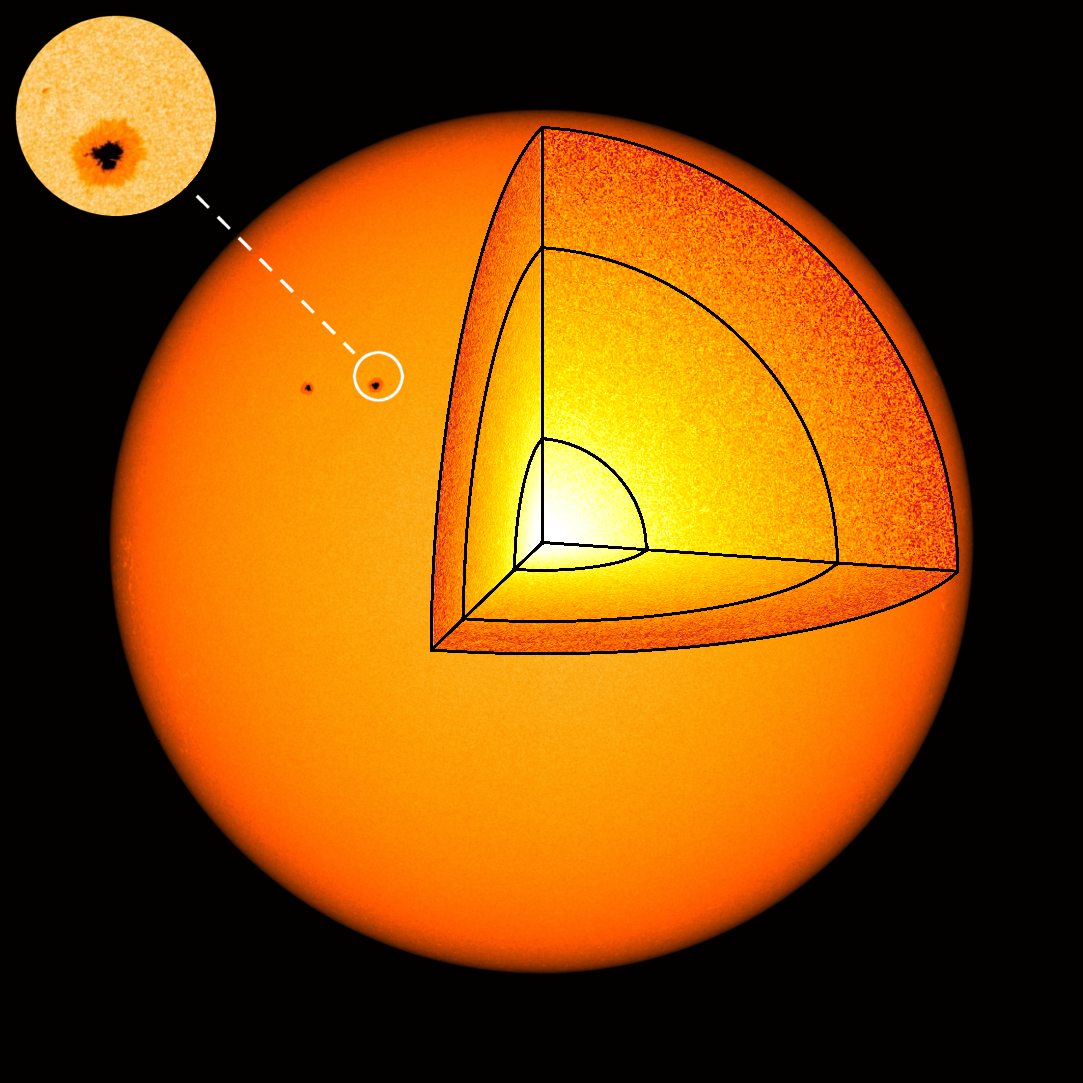
\includegraphics[width=0.6\textwidth]{images/own_figures/sun_interior_HMIIC.png}
	}{
		\caption{Image of the photosphere together with a schema of the solar interior structure. The inset shows the granular surface with a sunspot. The figure is based on a SDO/HMI continuum image from 20~March~2016; credit: NASA/SDO and the AIA, EVE and HMI science teams.}
		\label{fig:sun_interior_HMIIC}
	}
\end{figure}

%%% chromosphere + corona + CMEs
Above the photosphere at the base of the chromosphere the temperature declines to its solar minimum of \SI{3800}{\K} until it raises to \numrange{1}{3}~million~kelvins in the corona (cite? 2.4~GK Billings1959). Up to now it is not fully understood why the corona is so much hotter than the underlying chromosphere---this question is known as the coronal heating problem (cite?). The energy transfer mechanisms of choice are magnetic reconnections, wave heating and type~II spicules or a combination of these.

The chromosphere is a \SI{2000}{\km} thick region whose features (numerous spicules, filaments and prominences) can range far into the corona. They consist of by the solar magnetic field channeled chromospheric material, which is enveloped by a thin transition region where the temperature jumps up from ?\SIrange{20000}{35000}{\K} to coronal temperatures (cite?). Reconnection of magnetic field lines can result in the eruption of filaments into the corona and beyond, termed coronal mass ejections (CMEs) (see also Section~XX...). Details of chromospheric features are shown in \autoref{fig:sun_atmosphere}.

%%% coronal holes
The Sun's atmosphere is dominated by the varying small- and large-scale solar magnetic field configuration. There are regions where the magnetic field lines arc back to the surface and regions with open field lines. In the latter areas the coronal plasma can---guided by the field---escape into space. Thus these coronal areas are less dense, cooler and therefore appear darker in extreme ultraviolet (EUV) and are called coronal holes (more in Section~XX...). In \autoref{fig:sun_atmosphere} a coronal hole is located at the solar south pole.
\begin{figure}[htb]
	%\centering
	\fcapside[\FBwidth]{
		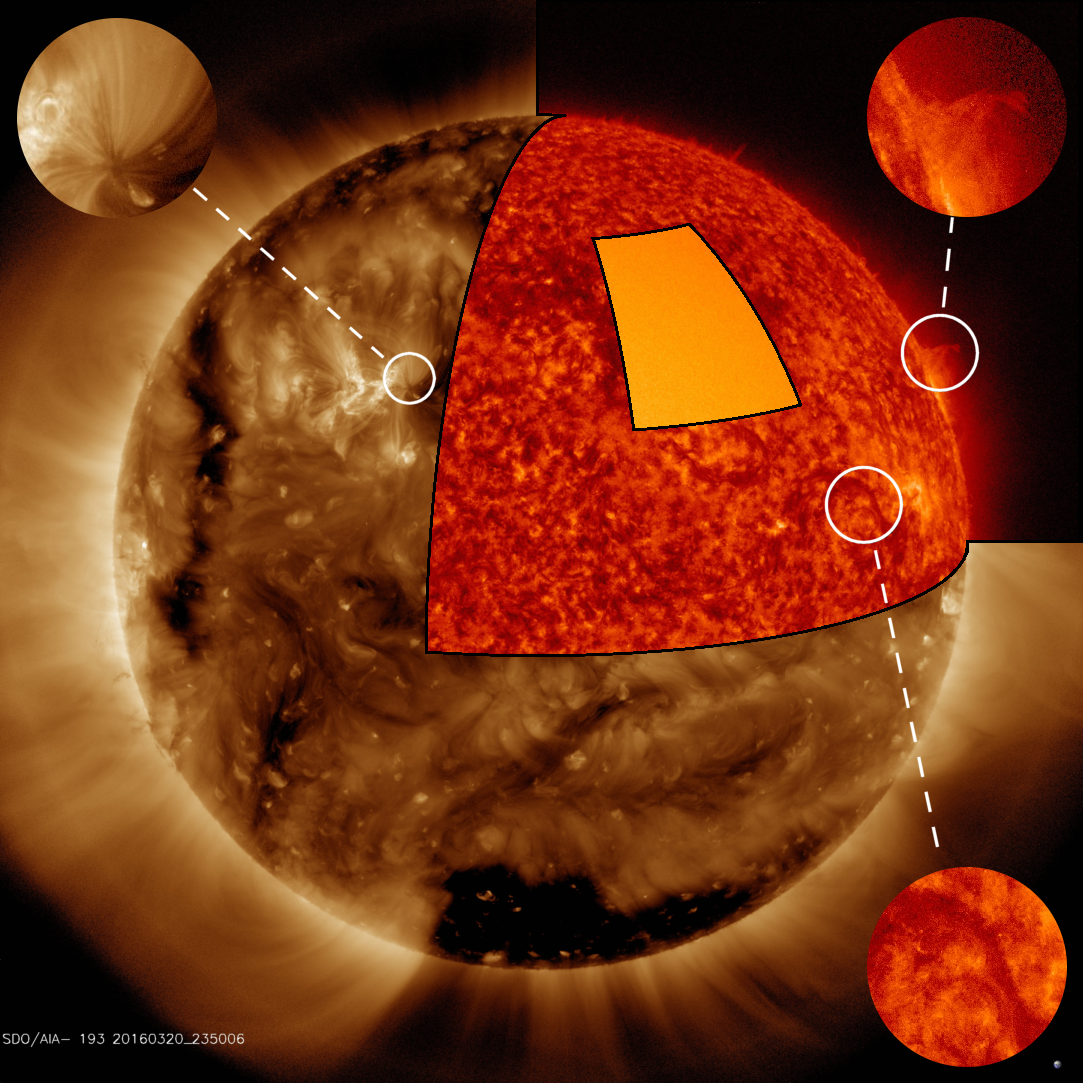
\includegraphics[width=0.6\textwidth]{images/own_figures/sun_atmosphere.png}
	}{
		\caption{Composite image of the solar atmosphere and some of its features. Corona, chromosphere and photosphere are seen in wavelengths of \SI{193}{\angstrom}, \SI{304}{\angstrom} and continu\-um. On the northern limb chromospheric spicules are visible. The enlargements on the right show a prominence and a filament. The dark region at the south pole is a coronal hole. The left inset shows details of the active region belonging to the sunspots in \autoref{fig:sun_interior_HMIIC}. The figure is based on SDO/AIA images from 20~March~2016; credit: NASA/SDO and the AIA, EVE and HMI science teams.}
		\label{fig:sun_atmosphere}
	}
\end{figure}

%%% corona
From Earth the faint corona and chromosphere can only be observed during eclipses, because of the brightness of the solar disk. There are three effects contributing to the visibility of the corona, photon scattering off free electrons and dust particles, and ion spectral emission lines (K-, F- and E"~corona).
% the so-called K-, F- and E"~corona (K kontinuierlich, F Fraunhofer, E emission).\\
% K-corona: photon scattering off free electrons --> coronagraphs\\
% F-corona: photon scattering off dust particles; contains Fraunhofer absorption lines; expands in ecliptic as zodiacal light --> coronagraphs\\
% E-corona: ion spectral emission lines; reveals coronal composition --> images\\
The image of a solar eclipse reveals the by the magnetic field shaped coronal plasma and features of the red chromosphere, pictured in \autoref{fig:Tse2008_500_mo1}.\\
\begin{figure}[htb]
	%\centering
	\fcapside[\FBwidth]{
		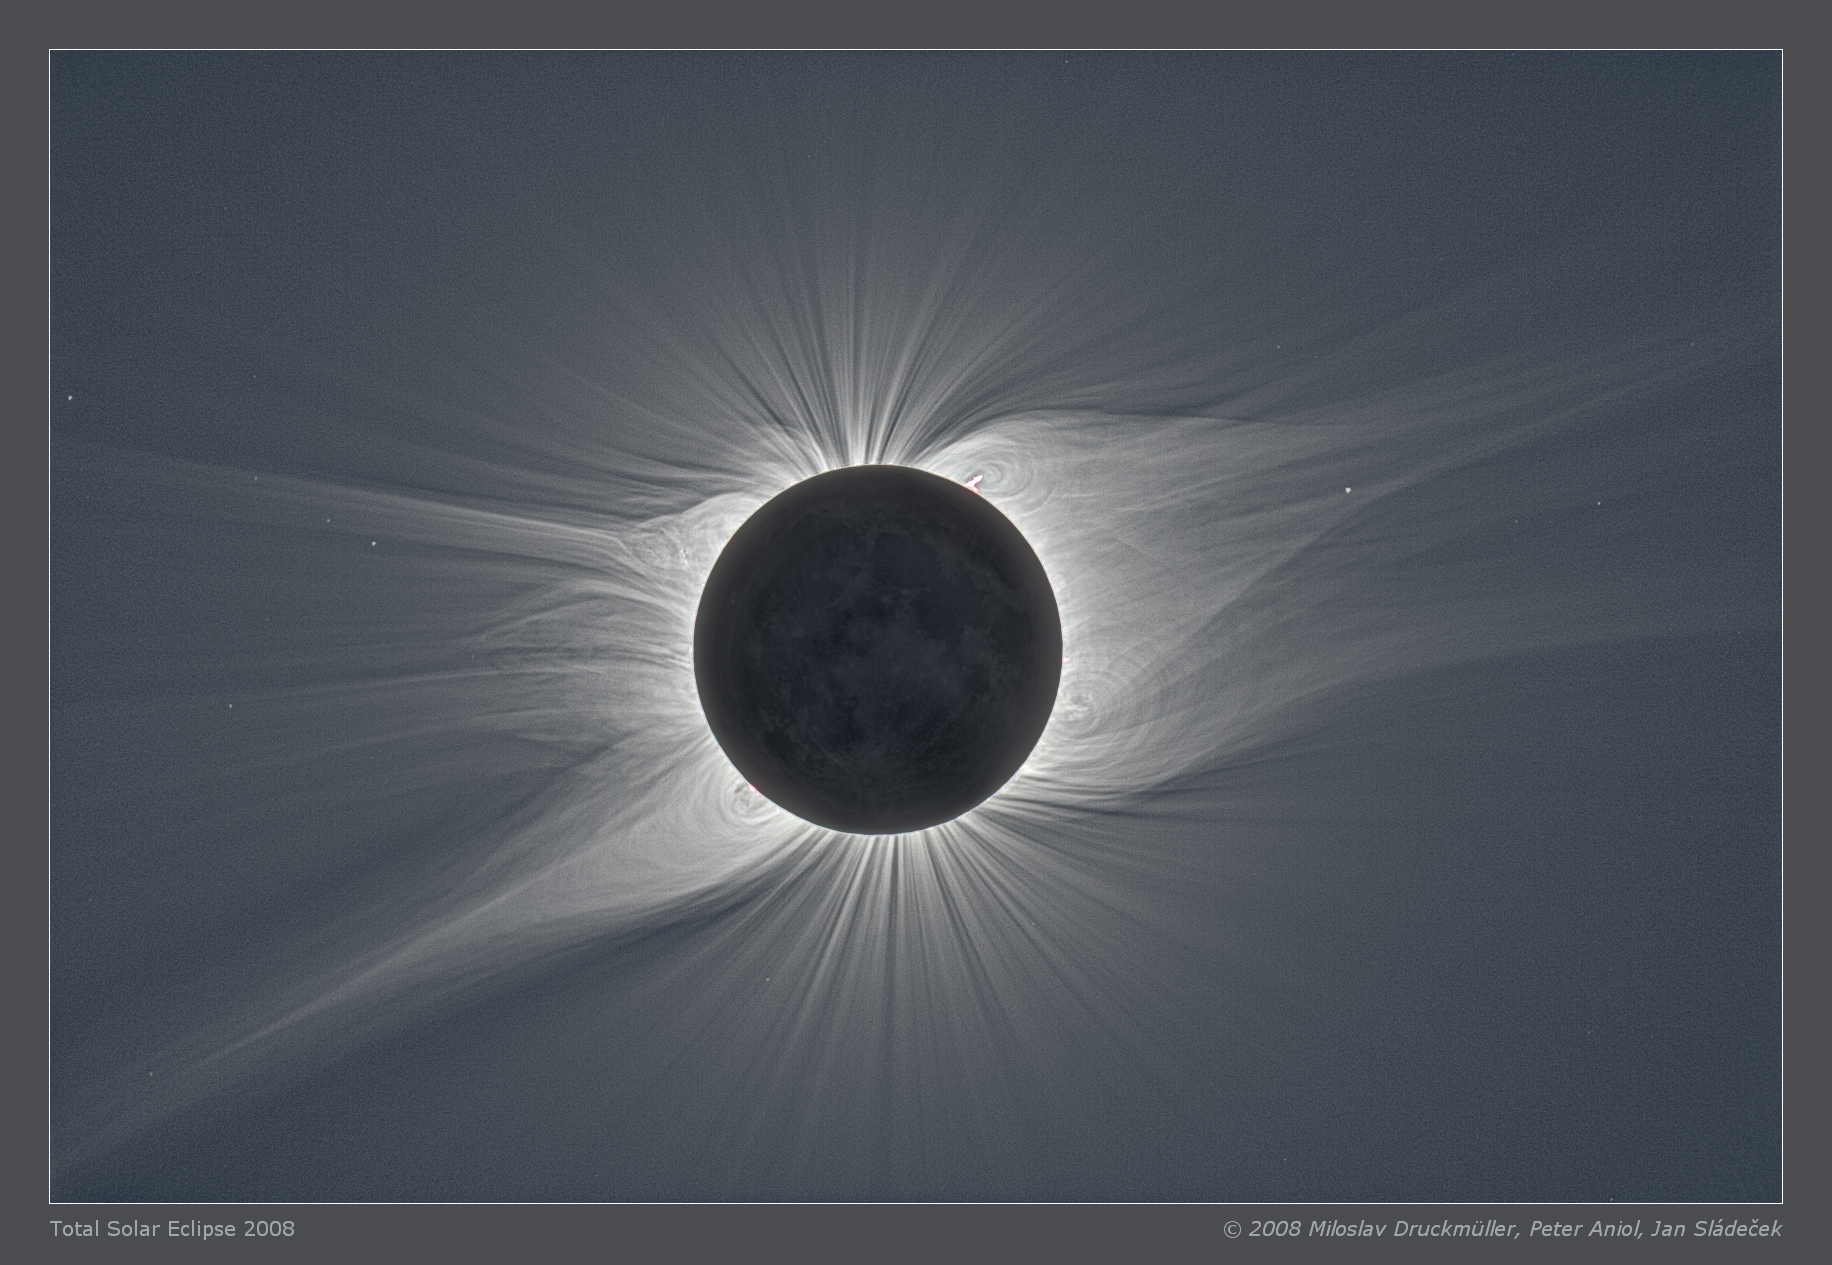
\includegraphics[width=0.6\textwidth]{images/Tse2008_500_mo1.png}
	}{
		\caption{Total solar eclipse image of the inner corona up to 5~solar radii. The picture was taken in Mongolia, 1~August~2008 and is processed from multiple images. Visible are the for a quiet Sun in cycle minimum typical magnetic field's dipole structure and the equatorial streamer belt. Credit: Miloslav Druckmüller, Peter Aniol, Jan Sládeček, 2008. get permission and preferred citation style... into acknowledgments? \url{http://www.zam.fme.vutbr.cz/~druck/Eclipse/}}
		\label{fig:Tse2008_500_mo1}
	}
\end{figure}
%figure source: http://www.zam.fme.vutbr.cz/~druck/Eclipse/Ecl2008m/Tse2008_500_mo1/Hr/Tse2008_500_mo1.png

%%% solar wind + heliosphere
Because of the high coronal temperatures, plasma escapes from the solar gravitational field \citep{Parker1958} with velocities of \SIrange{200}{800}{\km\per\s}. Its acceleration is linked to the coronal heating and its exact location and process remain an open question (cite?). At a distance of a few solar radii (?4--20) the magnetic field becomes too weak to guide the coronal plasma. From this source surface the solar wind flows radially outward into space until it reaches the termination shock, spanning the heliosphere. Eventually it collides with the local interstellar medium, creating the heliopause. The heliosphere is expected to be a bubble of teardrop shape (and may be led by a bow shock), caused by the Sun's relative velocity of \SI{23}{\km\per\s} to the local interstellar medium \citep{Owens2013}. Measurements of the Voyager~1 and 2 spacecraft indicate their passage of the termination shock at about \SI{94}{\au} and \SI{84}{\au}, entering the heliosheath region \citep{Owens2013}. \citet{Gurnett2013} report that in 2012 Voyager~1 actually crossed the heliopause into interstellar space at a solar distance of \SI{121}{\au}. \autoref{fig:Owens2013_Heliosphere_screenshot} illustrates the heliosphere and its surrounding flow structure.\\
\begin{figure}[htb]
	%\centering
	\fcapside[\FBwidth]{
		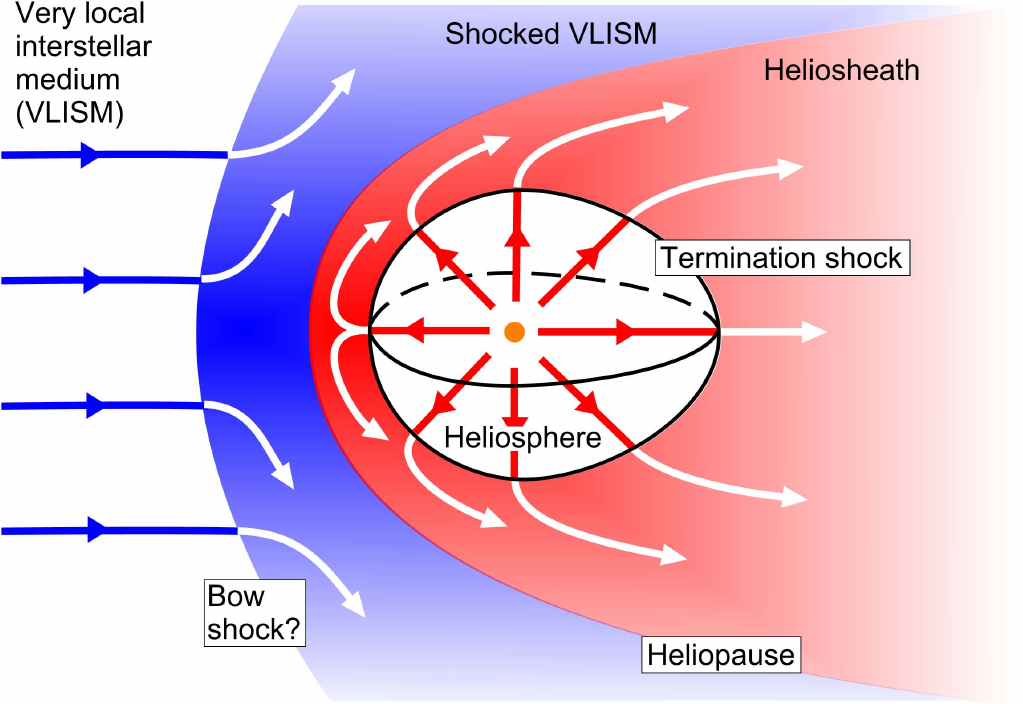
\includegraphics[width=0.6\textwidth]{images/Owens2013_Heliosphere_screenshot.png}
	}{
		\caption{Schema of the heliosphere and its surrounding flow structure. The heliosphere is formed by the interaction of the solar wind with the local interstellar medium at the heliopause. \citep[Fig.~9]{Owens2013} get permission...}
		\label{fig:Owens2013_Heliosphere_screenshot}
	}
\end{figure}

%%% solar wind influence + space weather
On its way outwards through the solar system the solar wind, carrying the solar magnetic field, interacts with the planets, their magnetic fields and other solar system bodies. These interactions have various effects, for instance disturbances in planetary magnetic fields with appearance of aurorae and enhanced radiation, atmospheric losses and stripping of cometary tails. Some of these effects can have disruptive consequences for humans and their technology. The topic of space weather effects is further addressed in \autoref{sec:space_weather}. The magnitude of these effects highly depend on spatial and temporal variations in the solar wind which are rooted in the dynamics of the solar magnetic field.\\

%%%%%%%%%%%%%%%%%%%%%%%%%%%%%
%\section{Stars/Beginning}
% introduction leading to stars; beginning from universe/big bang\\
% gravitational contraction of rotating nebula\\
% -> fusion burning; energy production\\
% In its core it fuses hydrogen to helium; 15.7~million~K; inner 25~\%\\
% energy transport -> radiation zone; up to 70~\%\\
% tachocline ~2~million~K\\
% energy transport by convection -> convection zone; up to surface\\
% convective granulation\\
% photoshere 4400--6600~K, effective black body temperature 5777~K; spectral class\\
% (herzsprung russell diagram)\\
% chromosphere... (solar atmosphere figure)\\
% transition region\\
%corona 1--3~million~K temperature (coronal heating problem)\\
% coronal holes: open magnetic field lines, solar wind\\
% heliosphere, shock with interstellar medium (ISM); Voyager\\

%%%%%%%%%%%%%%%%%%%%%%%%%%%%%
%big bang
%to formation of stars
%to ISM in our galaxy
%to formation of Sun
%Sun's inner structure (energy production and transport)
%its surface (radiation, spectral class)
%its outer structure (chromosphere, corona, solar wind, heliosphere)
%its heliosphere (termination shock with ISM, Voyager measurements)
%%%%%%%%%%%%%%%%%%%%%%%%%%%%%


\section{Solar dynamics}
\label{sec:solar_dynamics}

%%% differential rotation + solar magnetic field origin
The spin conservation of the contracting molecular cloud led to a rotation of the Sun with a current average period of about 25~days. The radial convective motion within the solar interior above the tachocline leads to a transport of momentum away from the rotation axis and therefore to a faster equatorial rotation in the convection zone \citep{Miesch2005}. This differential rotation is visible on the surface and was first discovered from sunspot observations. %in 1630 https://en.wikipedia.org/wiki/Solar_rotation
With a rotation period of about 34~days the poles have a lag of almost 9~days (for further information on solar rotation see appendix \autoref{sec:solar_rotation}). The differential rotation in the solar interior can be inferred from helioseismological observations, as seen in \autoref{fig:Miesch2005_fig1a_interior_diff_rot}. The resulting large rotational shear at the tachocline is believed to generate dynamo processes, creating the major part of the solar magnetic field \citep{Miesch2005}.\\
%Angular velocity profile in the solar interior inferred from helioseismology (after Thompson et al., 2003). In panel (a), a 2D (latitude-radius) rotational inversion is shown based on the subtractive optimally localized averaging (SOLA) technique. All inversions are based on data from the Michelson Doppler Imager (MDI) instrument aboard the SOHO spacecraft, averaged over 144 days. Inversions become unreliable close to the rotation axis, represented by white areas in panel (a). Note also that global modes are only sensitive to the rotation component which is symmetric about the equator (courtesy M.J. Thompson \& J. Christensen-Dalsgaard).

\begin{figure}[htb]
	\begin{floatrow}
		\ffigbox{	%[\FBwidth][]{
			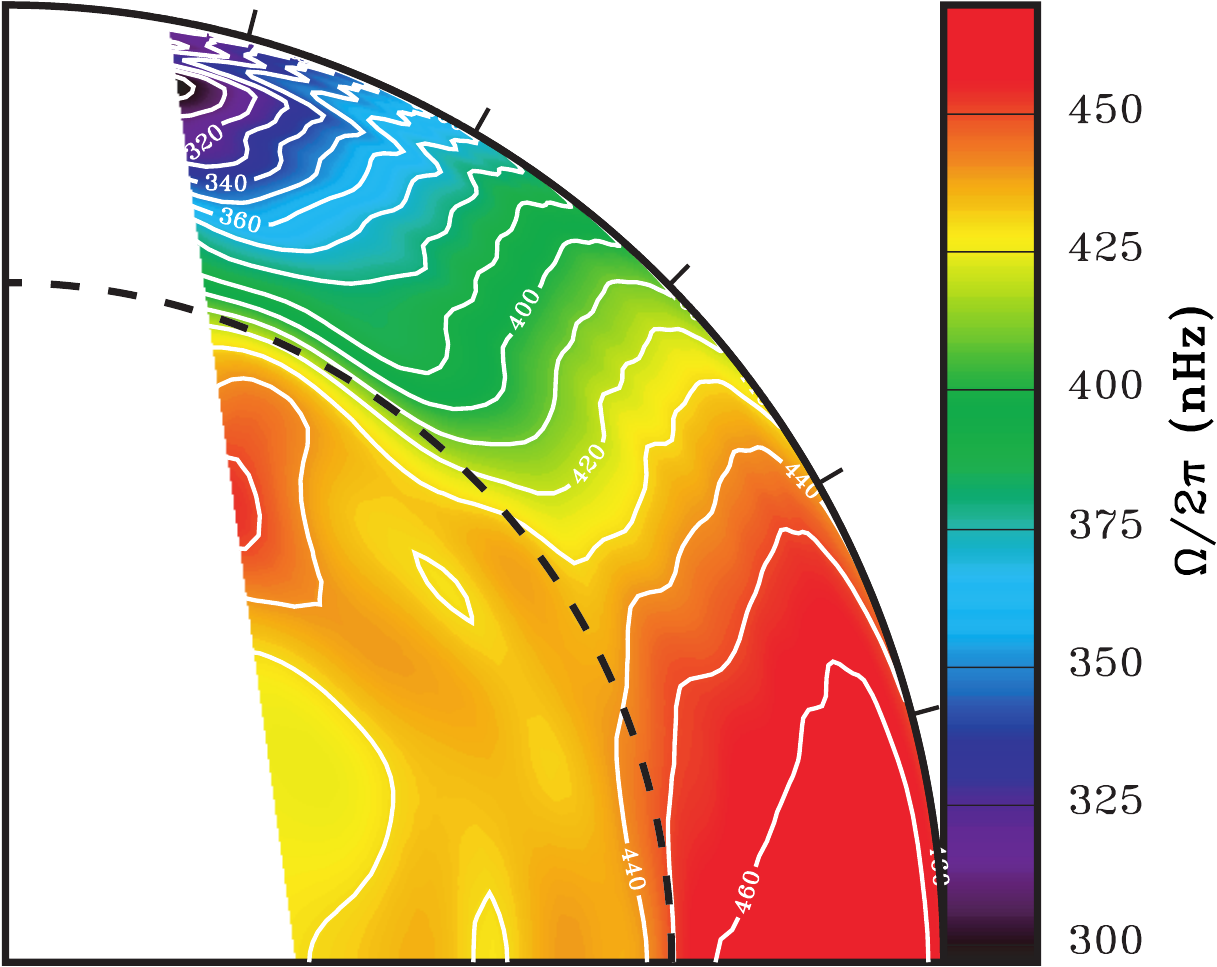
\includegraphics[width=0.5\textwidth]{images/Miesch2005_fig1a_interior_diff_rot.png}
		}{
			\caption{Angular rotation velocity in the solar interior. The radiation zone has a nearly solid rotation. Above the tachocline (dashed line) begins the differential rotation of the convection zone. The angular velocity is inferred from helioseismology via observations from the Michelson Doppler Imager (MDI) at the Solar and Heliospheric Observatory (SOHO) spacecraft. \citep[Fig.~3]{Thompson2003} get permission...}
			%(\citet[Fig.~1\,a]{Miesch2005}; based on \citet[Fig.~3]{Thompson2003})
			\label{fig:Miesch2005_fig1a_interior_diff_rot}
		}
		\ffigbox{
			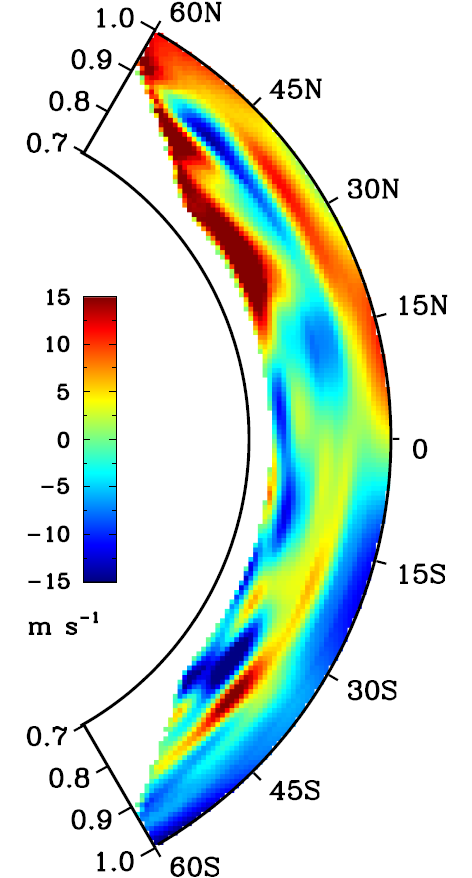
\includegraphics[width=0.28\textwidth]{images/Zhao2013_meridional_flow.png}
		}{
			\caption{Meridional flow velocity profile in part of the convection zone. Positive values are directed towards north. The velocity is inferred from helioseismology via observations from the Helioseismic Magnetic Imager (HMI) at the Solar Dynamics Observatory (SDO) spacecraft. \citep[Fig.~4\,a]{Zhao2013} get permission...}
			\label{fig:Zhao2013_meridional_flow}
		}
	\end{floatrow}
\end{figure}

%%% convection cycle + solar magnetic field + solar cycle
Helioseismic measurements reveal that the large-scale convective flow is agglomerated into large convection cells with slow meridional flows of a few \si{\m\per\s}. A poleward subsurface flow and equatorward backflow beneath is detected within each hemisphere, see \autoref{fig:Zhao2013_meridional_flow}. The cells have a convection cycle of about 22~years (cite...). As the magnetic field is carried by the plasma, it emerges at the surface with the same periodicity. Within one period the surface magnetic field configuration changes from a dipole structure to a reversed dipole structure with opposite polarity, thus the transition time from one dipole state to the next lasts about 11~years. In the transition phase magnetic flux emerges in belts above and below the solar equator, resulting in a multipolar structured magnetic field.\\

%%% sunspots
Since regions of strong magnetic flux are visible as sunspots on the photosphere, they were known well before the common era by chinese and greek scholars. %greek sunspot observation: http://adsabs.harvard.edu/abs/2007JBAA..117..346V
Systematic sunspot observations exist since 1610, shortly after the invention of the telescope (cite?). In 1843 Schwabe discovered the 11-year periodicity in the sunspot occurence (cite?). To record solar cycles in 1848 Wolf (et al?) introduced the sunspot number (SSN) and cycle number (with the zeroth occuring in 1749) (cite?), see \autoref{fig:ROB_ssn_wolfmms}.\\
\begin{figure}[htb]
	%\centering
	\fcapside[\FBwidth]{
		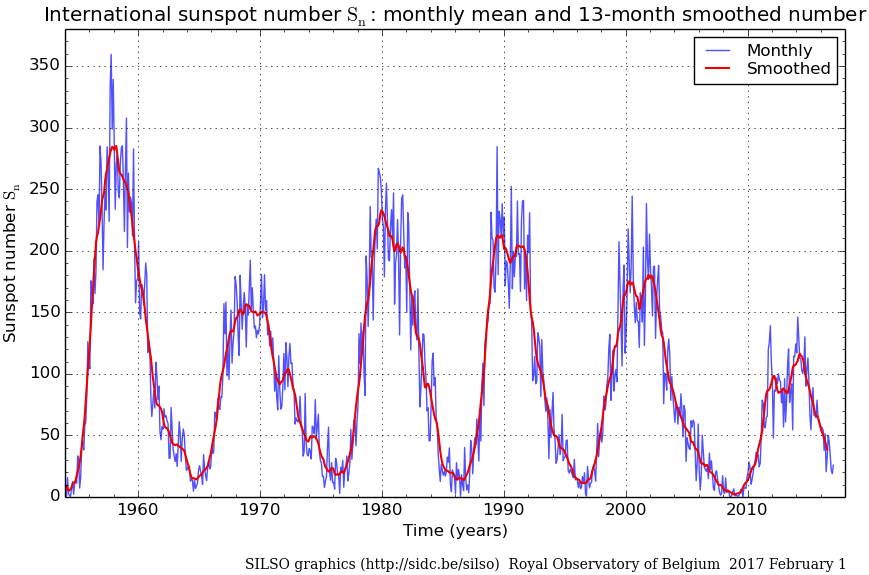
\includegraphics[width=0.6\textwidth]{images/ROB_ssn_wolfmms.png}
	}{
		\caption{The monthly mean sunspot number (blue) and 13-month smoothed monthly sunspot number (red) since 1954. Credit: SILSO data/image, Royal Observatory of Belgium, Brussels, \mbox{2017-02-01}. get permission... Update this figure before printing!!!}
		\label{fig:ROB_ssn_wolfmms}
	}
\end{figure}
%image from:	http://sidc.be/silso/
The large variations in cycle length ?(9--14~years) and intensity ?(0--350~Sn) make it difficult to predict the course of the next solar cycle (cite...).\\
lont-time variations like the Maunder minimum...\\

%butterfly
Observations of the surface radial magnetic field show the appearance of bipolar magnetic flux at belts of about \SI{+-20}{\degree} latitude at the beginning of a cycle and a shift to lower latitudes at the end of a cycle (magnetogram figure of sunspot?). Thus the plot of surface magnetic field over latitude and time reveals a butterfly pattern, see \autoref{fig:Hathaway_magbfly}. The emerging flux (its polarity alternates with each cycle) is carried by the slow meridional surface flow poleward, resulting in the polar field switch. The ordered dipole structure in solar cycle minimum leads to open polar field regions with coronal holes and a closed equatorial field belt.\\
\begin{figure}[htb]
	\centering
	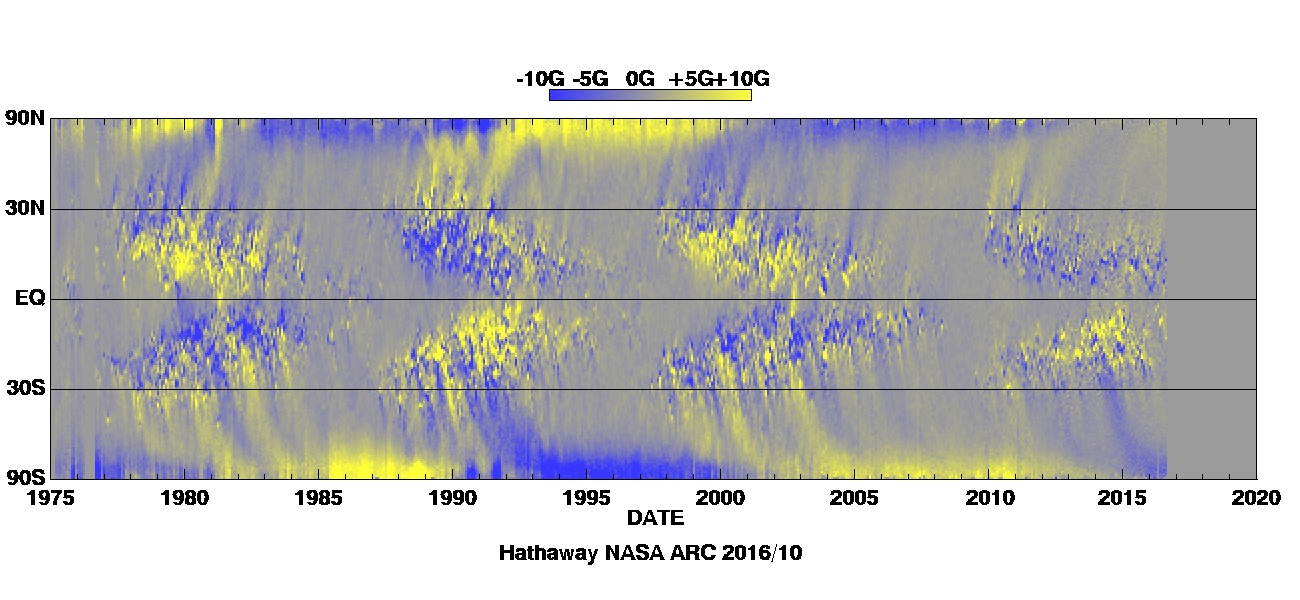
\includegraphics[width=\textwidth]{images/Hathaway_magbfly_201610.jpg}
	\caption{This magnetic butterfly diagram maps the synoptic radial magnetic field on the solar surface. Yellow represents an outward directed magnetic field (positive), blue inward (negative). The data is obtained from instruments on Kitt~Peak National Observatory and from the MDI at the SOHO spacecraft. Credit: David~Hathaway, NASA Marshall Space Flight Center; see also \citet[Fig.~17]{Hathaway2015}. Update this figure before printing!}
	\label{fig:Hathaway_magbfly}
\end{figure}
%figure source:	http://solarscience.msfc.nasa.gov/images/magbfly.jpg

compare with \autoref{fig:Tse2008_500_mo1}...\\

HMF geometry during maximum\\

fast solar wind emerges from CHs\\
\citet{Schwenn1983}: ``During the Skylab era in 1973/74 we learned that these high speed streams emerge from coronal holes (Hundhausen, 1977 and references therein).''\\

slow from closed field streamers\\

This is confirmed by the Ulysses spacecraft, which measured the solar wind speed in a polar orbit covering more than one solar cycle (\autoref{fig:McComas2008_Ulysses_orbit}).\\
\begin{figure}[htb]
	\centering
	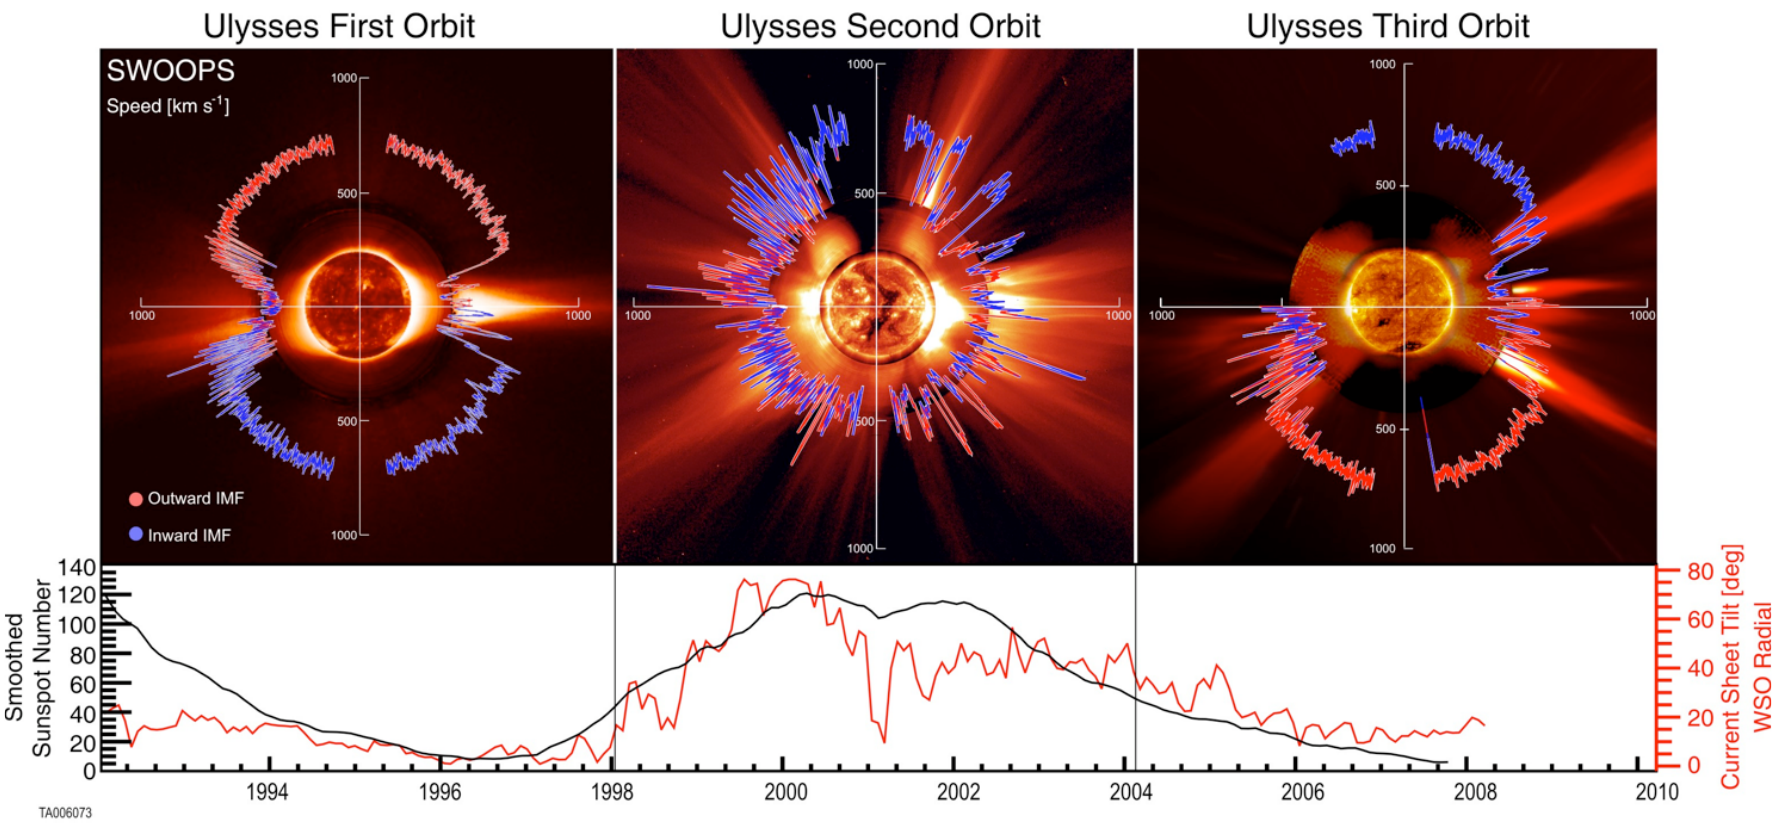
\includegraphics[width=\textwidth]{images/McComas2008_Ulysses_orbit_.png}
	\caption{Solar wind velocity and magnetic field polarity over latitude during low and high solar activity for the three orbits of the Ulysses spacecraft. The SSN and CS tilt angle are plotted as well. \citep[Fig.~1]{McComas2008}. ask for high res. image}
	\label{fig:McComas2008_Ulysses_orbit}
\end{figure}
%figure source: http://onlinelibrary.wiley.com/doi/10.1029/2003GL017136/full
%McComas2008: (a–c) Polar plots of the solar wind speed, colored by IMF polarity for Ulysses' three polar orbits colored to indicate measured magnetic polarity. In each, the earliest times are on the left (nine o'clock position) and progress around counterclockwise. (d) Contemporaneous values for the smoothed sunspot number (black) and heliospheric current sheet tilt (red), lined up to match Figures 1a–1c. In Figures 1a–1c, the solar wind speed is plotted over characteristic solar images for solar minimum for cycle 22 (8/17/96), solar maximum for cycle 23 (12/07/00), and solar minimum for cycle 23 (03/28/06). From the center out, we blend images from the Solar and Heliospheric Observatory (SOHO) Extreme ultraviolet Imaging Telescope (Fe XII at 1950 nm), the Mauna Loa K coronameter (700–950 nm), and the SOHO C2 white light coronagraph.

%++dynamics and magnetic field++\\
%rotating nebula to solar rotation\\
%rotation + convective motion -> differential rotation (first discovered by sunspot observations; helioseismology -> inner rotation, tachocline)\\
% meridional flow -> 22 year cycle || convective cells\\
% 22y convection cycle + magnetic field -> 11ys solar cycle (magnetic field activity cycle, polarity change, sunspot number)\\
SSN -> magnetic surface activity (butterfly diagram) => poloidal/toroidal field -> min/max polar CHs (quiet/active Sun figure) -> slow/fast sw pattern (Ulysses figure)) -> HMF (quiet B-field figure) -> Parker spiral (figure) -> solar wind\\

solar wind plasma composition and proberties -> visible solar wind structures (coronagraph image; with CME and streamer) -> stream interface (figure) -> in situ measurements (example in situ CIR/HSS plot)\\

stream interfaces (figure and link to previous CIR plot) -> HCS/HPS\\

CMEs (link to previous coronagraph image; in situ CME/MC plot; CME schema figure?)\\


switching between states of strong poloidal or toroidal field\\

differential rotation -> B-field\\
meridional flow -> solar cycle\\

dipole structure, open and closed field lines\\
polar coronal holes\\
streamer/equatorial streamer belt\\

solar wind\\

open field lines (coronal holes) -> HSSs\\
equatorial ballerina model -> CIRs (figure?)\\

%%% reconnections + CMEs
The solar differential rotation wraps the magnetic field lines, accumulating tension, leading eventually to relief with a magnetic reconfiguration by field line reconnections.\\
--> release of much energy --> flares, CMEs\\


solar wind's impact on Earth\\

the rotation axis is tilted from the normal of the ecliptic by $i_\odot = 7.25$\textdegree{} \citep{USNO2015} (refer to or put into appendix??).\\ %USNO2015 C3

%%%%%%%%%%%%%%%%%%%%%%%%%%%%%%%%%


\section{Solar wind}
\label{sec:solar_wind}

see Kivelson1995, p14+91\\
first observed at solar eclipses?, before? deduced by Parker from theory/Carrington from geomagnetic storms?\\

discovered via eclipses?\\
see eclipse photo from Druckmüller \autoref{fig:Tse2008_500_mo1}\\

in 1958 Parker predicted/postulated the solar wind \citep{Parker1958}\\
expanding isothermal atmosphere (solar wind model)\\
continuous supersonic radial outflow of plasma\\
-> also Parker spiral of HMF (see \autoref{fig:Owens2013_PFSS_Sectors_screenshot})


\section{Heliospheric magnetic field}	%better: interplanetary magnetic field??
%\label{sec:heliospheric_magnetic_field}

reviews: \citet{Balogh2009} (for heliosheath), \citet{Owens2013}\\

Winterhalter1994 The heliospheric plasma sheet:\\
"the narrow heliospheric current sheet (ca. 3000--10000 km thick), together with the heliospheric plasma sheet in which it is embedded. The heliospheric plasma sheet region is identified by a significantly enhanced plasma beta caused by density enhancements and diminished magnetic field strength and is about 20 to 30 times the thickness of the current sheet."\\
heliospheric current sheet (HCS)\\
heliospheric plasma sheet (HPS)\\
ballerina model... (search figure...)\\

%Cranmer2005:
%?insert their figure 1
Photosphere: magnetic bright points (MBP) 1--2~kG\\ %Cranmer2005
their convective motion result in wavelike fluctuations of the thin tubes\\
low chromosphere: thin flux tubes expand laterally and merge to a homogeneous network field\\
below the chromosphere-corona transition region: the network magnetic field expands laterally and merges again to a large-scale canopy (image)\\

[above the Alfv\'en critical point---where the wind speed equals the local Alfv\'en speed at about 10~$R_\odot$---both the inward and outward modes are advected (advect: convect horizontally) outward with the wind\\
superradially expanding magnetic flux tube\\
\citep{Cranmer2005}]\\
see also paper citations...\\

analytical solar magnetic field model for solar minimum conditions \citep{Banaszkiewicz1998}\\
dipole plus quadrupole plus current sheet (DQCS) solar magnetic field model\\
The DQCS model with its quadrupole part having a direct link from the solar equator to infinity along the equatorial plane and current sheet. (see \autoref{fig:Banaszkiewicz1998_DQCS_model_raw}) \citep{Banaszkiewicz1998}\\
compare with field geometry from eclipse \autoref{fig:Tse2008_500_mo1}...\\
\begin{figure}[htb]
	\begin{floatrow}
		\ffigbox{
			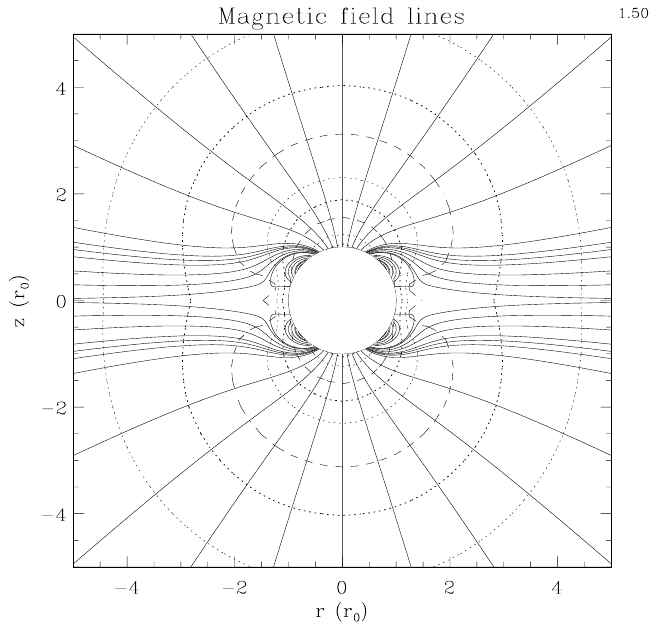
\includegraphics[width=0.45\textwidth]{images/Banaszkiewicz1998_DQCS_model_raw.png}
		}{
			\caption{Solar magnetic field geometry from the DQCS model with field lines (solid) and constant field strength surfaces (dashed). The quadrupole part allows equatorial outflows along the current sheet. \citep[Fig.~3]{Banaszkiewicz1998} get permission...}
			\label{fig:Banaszkiewicz1998_DQCS_model_raw}
		}
		\ffigbox{
			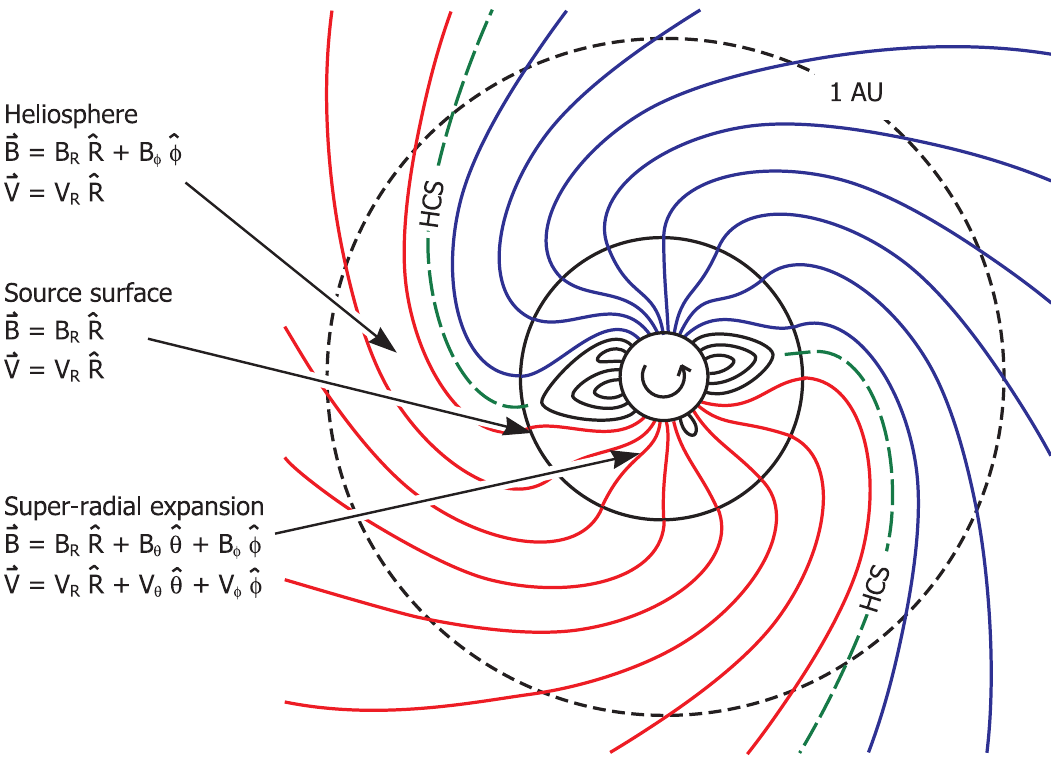
\includegraphics[width=\Xhsize]{images/Owens2013_PFSS_Sectors_screenshot.png}
		}{
			\caption{Illustration of the solar magnetic field Parker spiral formation by rotation of the solar wind source surface. Between solar wind flows of opposite magnetic field polarity a heliospheric current sheet (HCS) forms. (\citet[Fig.~1]{Owens2013}, adapted from \citet[Fig.~1]{Schatten1969}) get permission...}
			\label{fig:Owens2013_PFSS_Sectors_screenshot}
		}
	\end{floatrow}
\end{figure}

Parker spiral, source surface and HCS, see \autoref{fig:Owens2013_PFSS_Sectors_screenshot}\\
%A sketch of the steady-state solar magnetic field in the ecliptic plane. Close to the Sun, in a spatial region approximately bounding the solar corona, the magnetic field dominates the plasma flow and undergoes significant non-radial (or super-radial) expansion with height. At the source surface, typically taken to be a few solar radii, the pressure-driven expansion of the solar wind dominates and both the field and flow both become purely radial. In the heliosphere, rotation of the HMF footpoints within a radial solar wind flow generates an azimuthal component of the HMF, leading to a archimedean spiral geometry. Regions of opposite HMF polarity, shown as red and blue lines, are separated by the heliospheric current sheet (HCS), shown as the green dashed line. Image adapted from Schatten et al. (1969).

MHD simulations based on Voyager~1 and 2 measurements within the heliosheath indicate the formation of magnetic bubbles (reconnected sector regions) at the sector boundary caused by the compression before the heliopause, flowing away to the heliosheath tail \citep{Opher2011}.\\
%Opher2011: Is the Magnetic Field in the Heliosheath Laminar or a Turbulent Sea of Bubbles?


\section{Solar wind properties and structures}

list event/structure types\\
solar wind structures source regions: sunspots/active regions, coronal holes, filaments\\


\subsection{Solar wind plasma}
\label{sec:solar_wind_plasma}

Plasma in general (properties (H/He/metal composition; see paper...), Plasma-beta, etc.)\\
	solar wind properties, slow/fast wind, MHD waves (Alfv\'en waves)\\

special events/configurations, which can appear (CIRs, HCS/HPS, etc.)
HSS, sector boundaries, CIRs, CMEs\\


\subsection{Slow solar wind}

regions with closed lines\\
trapped plasma, slow solar wind from streamers\\


\subsection{High speed streams}

regions with open lines\\
coronal holes as sources of fast sw\\

sw plot of HSS with CIR to refer to\\


\subsection{Stream interaction regions}

Streams of fast wind catch slow wind\\
-> compressions, shocks, deflections\\

Corotating interaction regions (CIRs)\\
Stream interaction regions (SIRs)\\

formation of stream interface and stream deflection, see \autoref{fig:Owens2013_CIR_2panel_screenshot}\\
%A sketch of a stream interaction region. Left: Looking down on the ecliptic plane. Magnetic field lines within fast (slow) wind, shown in red (blue), become aligned with the stream interface by the reverse (forward) wave. Right: a view from Earth. The magnetic axis, M, and therefore the wind speed belts, are inclined to the rotation axis, R. The point in the heliosphere at which fast wind is able to catch up to the slow wind ahead of it is the stream interface (SI), which forms a spiral front in the heliosphere, shown as the black-outlined curved surface. In the frame of reference of the SI, both fast and slow wind flow toward the SI. Fast (slow) wind, shown by the red (blue) arrow, is slowed (accelerated) and deflected along the SI in the direction counter to (along) solar rotation. Right panel adapted from Pizzo (1991).
\begin{figure}[htb]
	%\centering
	\fcapside[\FBwidth]{
		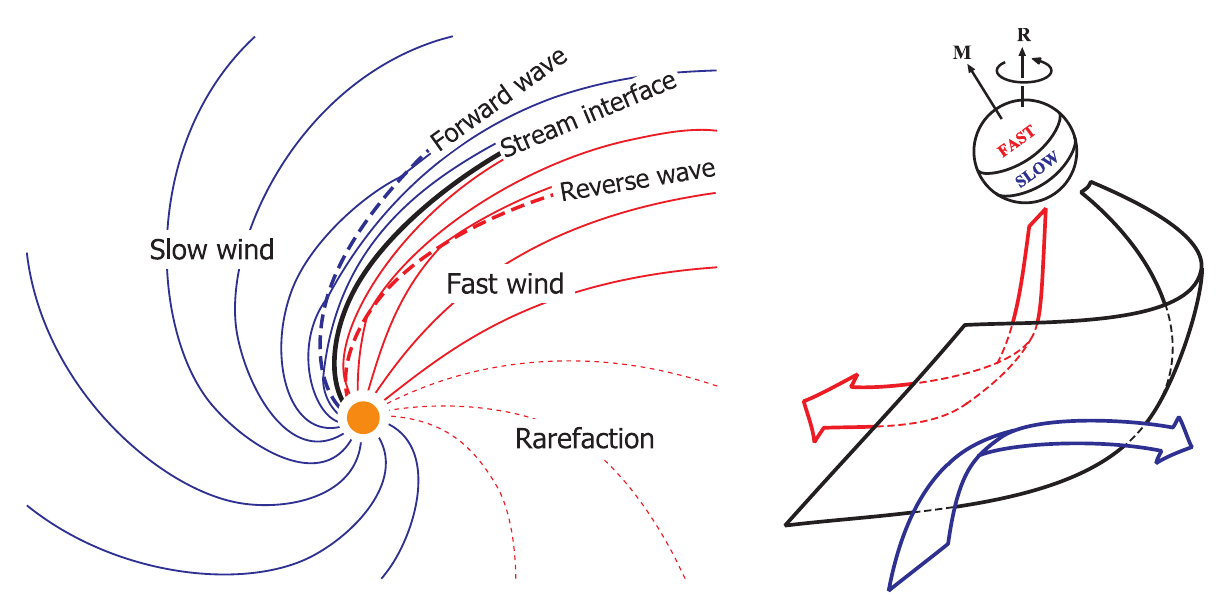
\includegraphics[width=0.6\textwidth]{images/Owens2013_CIR_2panel_screenshot.png}
	}{
		\caption{Schema of the formation of a stream interface (left) and deflection of streams (right), both generated from interactions between slow and fast solar wind. (\citet[Fig.~7]{Owens2013}; right panel adapted from \citet[Fig.~2]{Pizzo1991}) get permission...}
		\label{fig:Owens2013_CIR_2panel_screenshot}
	}
\end{figure}
refer to sw figure of CIR\\


\subsection{HCS / HPS}

from sector boundaries (ballerina skirt)\\


\subsection{Coronal mass ejections}
\label{sec:coronal_mass_ejections}

Coronal mass ejections (CMEs) (discovery (Carrington), definition (Hundthausen?), models, GCS (conception of 3-dim CME shape --> enables Earth arrival time forecast from modeled direction and velocity))\\

active regions:\\
sunspots, magnetic reconnections, flares, post-eruptive arcades\\

coronagraph figure of CME (COR2 image, SECCHI/STEREO)\\
in situ solar wind figure of same CME (recent one from 2016)\\

CME-plasma properties\\


\subsubsection{Magnetic clouds}
%\label{sec:magnetic_clouds}

magnetic cloud (MC); refer to in situ plot\\
See BS magnetic cloud model in analyses methods chapter
MVA...\\


\section{Space weather}
\label{sec:space_weather}

Solar wind influences the Earth's magnetosphere and can disturb sensitive technical systems\\
understanding its properties helps with prediction of events\\

influences on human infrastructure/technical systems\\

various space weather effects, for instance disturbances in magnetic fields, aurorae, episodes of enhanced radiation, atmospheric losses and stripping of cometary tails. figures of these effects?\\


\subsection{Solar influence on Earth}
\label{sec:solar_influence_on_earth}

Carrington made first connection between terrestrial magnetic field and solar flares. correct?\\

%see Bartels1962:
there are several types of solar-terrestrial relations, \citet{Bartels1962} listed:\\	%Zuordnung solarer Beobachtungen zu terrestrischen\\
a) irregular flare and CME effects (Carrington)\\
b) 11"~year solar cycle effects\\
c) 27"~day solar rotation effects\\
d) daily effects (x-ray and light)\\

seasonal effects from Earth orbital distance, inclination (solar rotation axis angle) and Earth tilt (get figure...)\\

solar wind and its species\\
solar radiation\\
solar energetic particles (SEPs)\\
gravitation\\

magnetosphere\\
ionosphere?\\
aurorae\\
geomagnetic storms (several days, from CMEs)\\
substorms (few hours, from CIRs??)\\

for humans and their technology important effects: enhanced radiation, geomagnetic storms\\
lovely, disruptive, dangerous consequences\\

at Earth the solar wind total energy flux ($1.45~\text{mW/m}^2$) is only about one millionth of the solar radiation flux (see \citet[p.~153]{Schwenn1990})\\


\subsection{Magnetosphere}
\label{sec:magnetosphere}

shape formed by dynamic pressure..., similar to heliosphere in ISM...\\

bow shock, magnetotail, magnetosheath, magnetopause\\
add ecliptic and terrestrial tilt angle; with plasmoid?\\
see \autoref{fig:heliosphere_image002}\\
\begin{figure}[htb]
	%\centering
	\fcapside[\FBwidth]{
		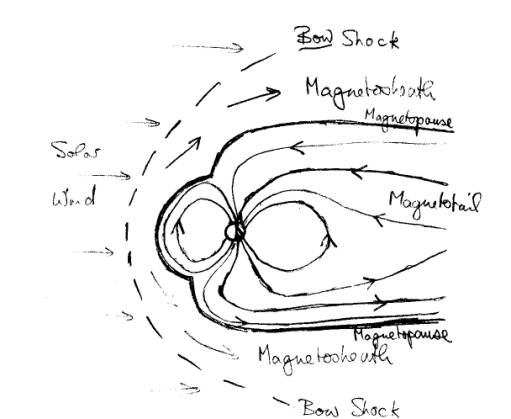
\includegraphics[width=0.5\textwidth]{images/heliosphere_image002.jpg}
	}{
		\caption{temp figure ``The cavity is called the magnetosphere. It has a relatively well-defined outer boundary, the magnetopause.''}
		\label{fig:heliosphere_image002}
	}
\end{figure}

turbulence with sw (KH or RT instabilities), see \autoref{sec:solar_wind_magnetosphere_coupling}\\

Earth magnetic field strength at a height of 36\,000~km (geostationary): ~100~nT\\
Earth magnetic field strength at the surface - equator: ~30\,000~nT - poles: ~60\,000~nT (cite?)\\

magnetopause = current layer??\\

two extreme cases of Bz orientation: parallel/antiparallel\\
compression/reconnection (with figure)\\

standoff distance:	\citep[p.~112]{Bothmer2007}
\begin{align}
	d = \frac{107.4}{1 R_\text{E}} (N V^2)^{-1/6}
\end{align}

Even in ``ancient'' times (when?) a correlation between solar particles and disturbances in the magnetosphere were known of (Bartels1962).\\

magnetosphere variations due to solar wind\\
magnetosphere protects from radiation (maybe from solar wind stripping atmosphere away?)\\

effects: aurorae, ...\\

ring current systems\\

definition of:\\
magnetic storm...\\
substorm...\\

subsection Ionosphere?\\
its variations due to solar radiation (day/night cycle and flares)\\
ionosphere -> TEC -> GNSS error\\


\subsection{Geomagnetic indices}
\label{sec:geomagnetic_indices}

%%% various indices
for Kp, AA and Dst read Section 7.4 in book \citet{Bothmer2007}...\\
Geomagnetic indices (variety of indices AA, AE, Dst, etc.)\\
Kp index, construction from 13 K stations... (-> look into early presentations)\\	%see GFZ Potsdam website
% http://isgi.unistra.fr/indices_kp.php (nice figure with Kp obs locations)
The Kp index is described in \autoref{sec:kp_index}.\\

AE - intensity of northern polar electrojet\\
Dst - intensity of magnetospheric ring current\\
Ring-Current Index Dst (read book Jursa1985 p. 4-31)\\


\subsection{Solar wind--magnetosphere coupling}
\label{sec:solar_wind_magnetosphere_coupling}

E"~field:	%VBth p124
\begin{align}
	\textbf{E}_\text{IMF?} = -\textbf{V} \times \textbf{B}_\text{IMF}
\end{align}
...derive from Lorentz force\\
(Because of high plasma conductivity the E"~field is not existent.)\\

Axford1964 viscous interaction (of turbulent nature, KH/RT instabilities, KH instabilities at the flanks of the magnetosphere) is a viable source of drag force/solar storm energy input into magnetosphere\\

Otto\&Nykyri1982 KH instabilities/vortices force magnetic reconnection even at northern IMF and are able to account for observed mass flux\\

\citet{Newell2007} and \citet{Newell2008}: coupling consists of merging and viscous part (reconnection and turbulence)\\
merging part: rate magnetic flux is opened at the magnetopause\\
viscous part: reconnection due to Kelvin-Helmholtz instabilies at the boundary\\

Merkin2013 MHD simulation of velocity shear at magnetosphere boundary with northern IMF; KH instabilities; double-vortex sheet structure\\


\chapter{Data}
\label{chap:data}

%COFI -- chapter outline and flow integration\\


\section{Instruments}
%\label{sec:instruments}

For analyzing the Sun and solar wind there are remote instruments (solar imager and coronagraphs) and in situ instruments (magnetometer and plasma detector).\\
Here the basic principles of latter are described, as we only use them...\\

several spectrometers with different energy ranges\\

isotope spectrometer - isotopic abundances of SEPs\\
ionic charge analyzer - charge state of SEPs\\
sw ion mass spectrometer - \\
sw ion composition spectrometer - \\
radio burst tracker\\


\subsection{Magnetometer}
%\label{sec:magnetometer}

Spacecraft nowadays carry two different magnetometer types, one for measuring the magnetic field direction and its strength and the other for observing the magnetic flux and detecting waves.\\

flux gate magnetometer -- two coils around core, one coil with alternating current, wich is compared with the induced current signal from the other; without external magnetic field both patterns match. the core is easier magnetized in direction of an existing external magnetic field -> patterns differ\\
search coil magnetometer -- a coil around a core; measures plasma waves\\

Because these magnetometer types are directional, they often are placed in two sets of triaxial configurations, attached on booms to decrease the influence of the spacecraft's own magnetic field.\\
L-> which is generated by surface charges?/electrons?/ionization?/the instruments?\\
%https://en.wikipedia.org/wiki/Spacecraft_magnetometer


\subsection{Plasma detector}
%\label{sec:plasma_detector}

A plasma detector measures the ion energy frequency distribution, which consists basically only of protons and alphas in solar wind (see \autoref{fig:ion_energy_spectrum_plot}). see also \autoref{sec:solar_wind_plasma}
\\
\begin{figure}[htb]
	%\centering
	\fcapside[\FBwidth]{
		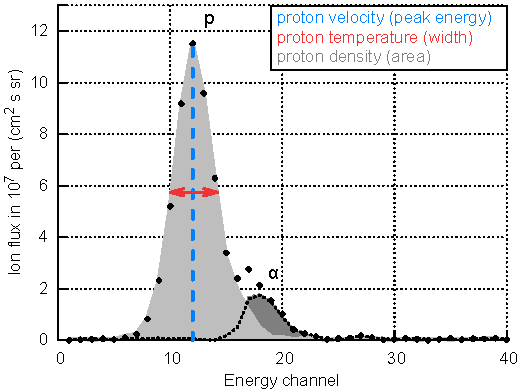
\includegraphics[width=0.5\textwidth]{images/gnuplots/ion_energy_spectrum_plot.pdf}
	}{
		\caption{Example of an ion energy spectrum with synthetic data. Here proton and helium (alpha) peaks are distinguishable...}
		\label{fig:ion_energy_spectrum_plot}
	}
\end{figure}
%figure adapted from source: http://www.goembel.biz/sun.html

From the energy spectrum the velocity, density and temperature an be derived.\\


average energy --> bulk velocity\\
distribution area --> number density\\
distribution width --> temperature\\

% source: ftp://spdf.gsfc.nasa.gov/pub/data/ulysses/plasma/swoops/ion/swoops_ion_users_guide_update_20030214.txt
% ``Plasma parameters are calculated by numerical integration of velocity-weighted
% ion distributions over an E/q range chosen to include the thermal proton and
% alpha-particle populations. Under extremely hot conditions, there can
% sometimes be some overlap between these populations. Additionally, during
% periods when the solar wind temperature is exceptionally low the experiment can
% not properly measure the temperature. Care has been taken to estimate the
% instrument background from channels that do not contain data, and the effects
% of background have been removed from the integration. The velocity space 
% resolution of the experiment is better in the energy dimension than in the
% angular dimensions.''


\section{Data sources}
%\label{sec:}

Spacecraft / data sets\\

Positions:\\
Earth:\\
	imager, magnetosphere\\
L1 - Lagrangian point:\\
	ACE (siehe auch space weather spacecraft Liste)\\
	Wind etc. (OMNI)\\
inner heliosphere:\\
	Helios~1 \& 2\\
outer heliosphere:\\
	Voyager~1 and 2\\
	Ulysses\\

also RT-data sources?\\


\subsection{Sunspot number}
%\label{sec:sunspot_number}

SSN history\\
add SSN figure of history incl. Maunder minimum?\\

SIDC/SILSO...\\
WDC-SILSO -- World Data Center-Sunspot Index and Long-term Solar Observations\\
%https://de.wikipedia.org/wiki/Sonnenfleck#Geschichte


\subsection{Kp index}
\label{sec:kp_index}

Kp index first introduced by \citet{Bartels1949}\\
it was maintained at the University of Göttingen...\\

insert figure of Kp musical diagram\\

mention IAGA...\\

The German Research Centre for Geosciences (GFZ) in Potsdam supplies indices of global geomagnetic activity, more precisely the Kp index and thereof derived indices. The GFZ provides historical and quicklook data of the indices via their website\footnote{GFZ website: \url{http://www.gfz-potsdam.de/sektion/erdmagnetfeld/daten-produkte-dienste/kp-index/} (existent in 2017-02-12)}.\\
list Kp derived indices\\
ap, Ap, K, Cp, ...\\


\subsection{OMNI data set}
\label{sec:omni_data_set}

a data set merged from different sources\\
The OMNI data \citep{King2005} were obtained from the GSFC/SPDF OMNIWeb interface.\\

from spacecraft located near the Lagrange point L1 upstream of Earth\\
time-shifted to the bow shock of the magnetosphere\\

OMNI2 H0 MRG1HR (1963-201308)
Cite from CDAweb: Hourly near-Earth solar wind magnetic field and plasma data, energetic proton fluxes (>~1 to >~60~MeV), and geomagnetic and solar activity indices.

NASA, Goddard Space Flight Center (GSFC), Space Physics Data Facility (SPDF): \url{http://spdf.gsfc.nasa.gov/}\\	%exintent in 2016-08-18
- Coordinated Data Analysis Web (CDAWeb): \url{http://cdaweb.gsfc.nasa.gov/}\\	%exintent in 2016-08-18
- OMNIWeb Plus: \url{http://omniweb.gsfc.nasa.gov/}\\	%exintent in 2016-08-18
%OMNIWeb Data Documentation: http://omniweb.gsfc.nasa.gov/html/ow_data.html


OMNI spacecraft data coverage (see also talk 2014-02-18)\\
see \autoref{fig:omni_data_coverage_1963-2013_plot}
\begin{figure}[htb]
	%\centering
	\fcapside[\FBwidth]{
		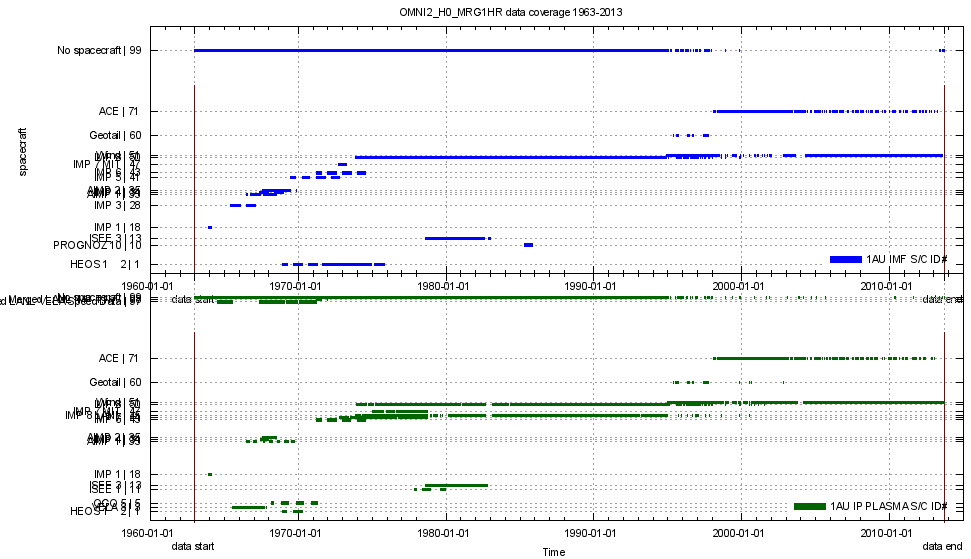
\includegraphics[width=0.5\textwidth]{images/gnuplots/omni_data_coverage_1963-2013_plot.png}
		\caption{OMNI intercalibrated multi-spacecraft data coverage per spacecraft. renew plot until 2016-11; integrate into 1 panel...}
	}{
		\label{fig:omni_data_coverage_1963-2013_plot}
	}
\end{figure}


\subsubsection{Advanced Composition Explorer}

s/c figure, launch date was 25 August 1997\\

MAG -- fluxgate magnetometer\\
SWEPAM\\	%https://sci-hub.ac/10.1023/A:1005040232597

data errors/gaps...\\

DSCOVR as replacement..., launched on 11 February 2015, NOAA's SWPC real-time solar wind prime source since 27 July 2016\\
\url{http://www.swpc.noaa.gov/products/real-time-solar-wind}\\


\subsubsection{Solar Wind Structures}

Solar Wind Structures (SWS) list\\
derived by Richardson.... from OMNI data (only?)

permission received.\\

%http://cedarweb.vsp.ucar.edu/wiki/index.php/Tools_and_Models:Solar_Wind_Structures
characterization of near-Earth solar wind structures since 1963\\
SWS lists \citep{Richardson2000} and \citep{Richardson2012}


\subsection{Helios probes}
\label{sec:helios_probes}

see Helios data readme.txt\\

two different fluxgate magnetometers and a search coil magnetometer\\

see \autoref{fig:MPS_Helios}
\begin{figure}[htb]
	\begin{floatrow}
		\ffigbox[\FBwidth][]{
			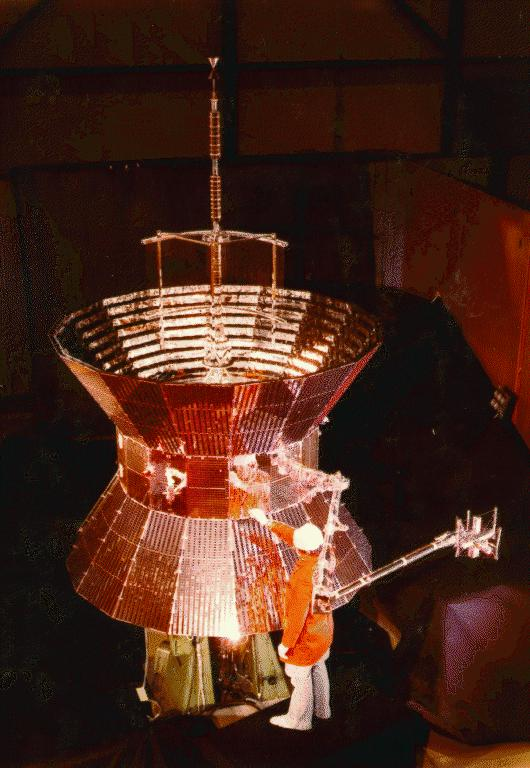
\includegraphics[width=0.3\textwidth]{images/MPS_Helios.jpg}
		}{
			\caption{One of the nearly identical twin Helios spacecraft. Credit: Max Planck Institute for Solar System Research. get permission...}
			\label{fig:MPS_Helios}
		}
		\ffigbox[\Xhsize]{
			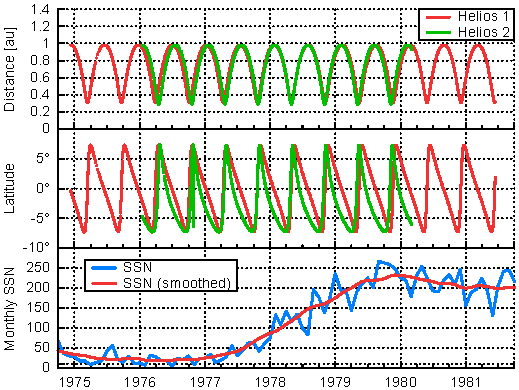
\includegraphics{images/gnuplots/Helios12_1h_r_b_ssn_plot.pdf}
		}{
			\caption{Plot of the Helios probes' solar distance and HGI latitude over their mission time, together with the monthly SSN and 13-month smoothed monthly SSN.}
			\label{fig:Helios12_1h_r_b_ssn_plot}
		}
	\end{floatrow}
\end{figure}

solar distance, HGI latitude and sunspot number during the Helios missions; see \autoref{fig:Helios12_1h_r_b_ssn_plot}\\

Helios orbit in the ecliptic plane (see \autoref{fig:Helios12_1h_magswe_ecliptic_plot}) and in the latitude polar plane (see \autoref{fig:Helios12_1h_magswe_polar_plot}); make 2-panel figure...\\
\begin{figure}[htb]
	\begin{floatrow}
		\ffigbox{
			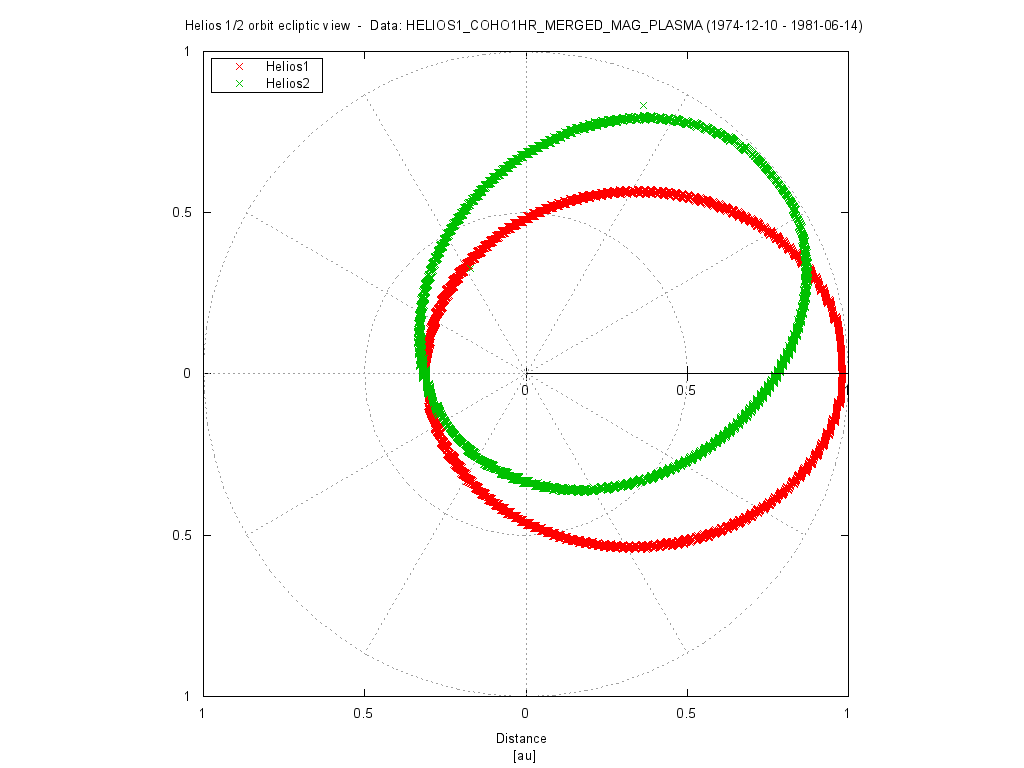
\includegraphics[width=0.45\textwidth]{images/gnuplots/Helios12_1h_magswe_ecliptic_plot.png}
		}{
			\caption{Plot of the Helios orbits in the ecliptic plane (left) and polar plane (right) (in HGI-coordinates). combine with polar plane plot...}
			\label{fig:Helios12_1h_magswe_ecliptic_plot}
		}
		\ffigbox{
			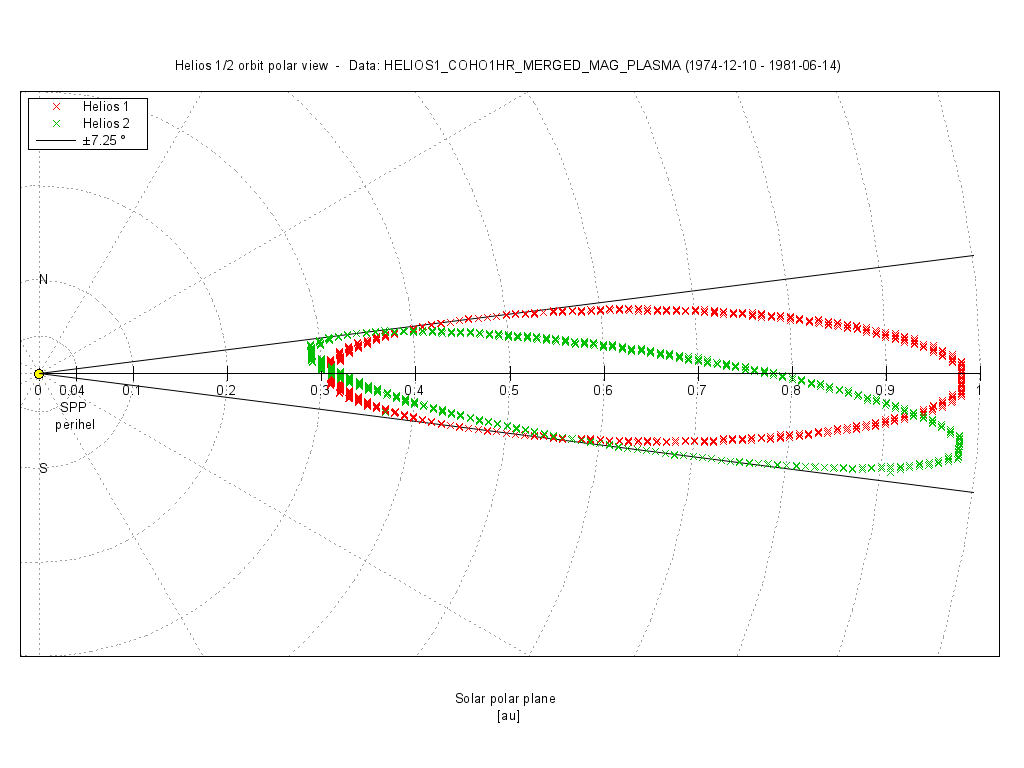
\includegraphics[width=\Xhsize]{images/gnuplots/Helios12_1h_magswe_polar_plot.png}
		}{
			\caption{combine with other plot...}
			\label{fig:Helios12_1h_magswe_polar_plot}
		}
	\end{floatrow}
\end{figure}

The Helios magnetic field and plasma data counts over solar distance are plotted in \autoref{fig:Helios12_1h_magswe_r-count_plot} and over latitude are plotted in \autoref{fig:latitude_frequency_plot}. build 2-panel figure...\\
\begin{figure}[htb]
	\begin{floatrow}
		\ffigbox{
			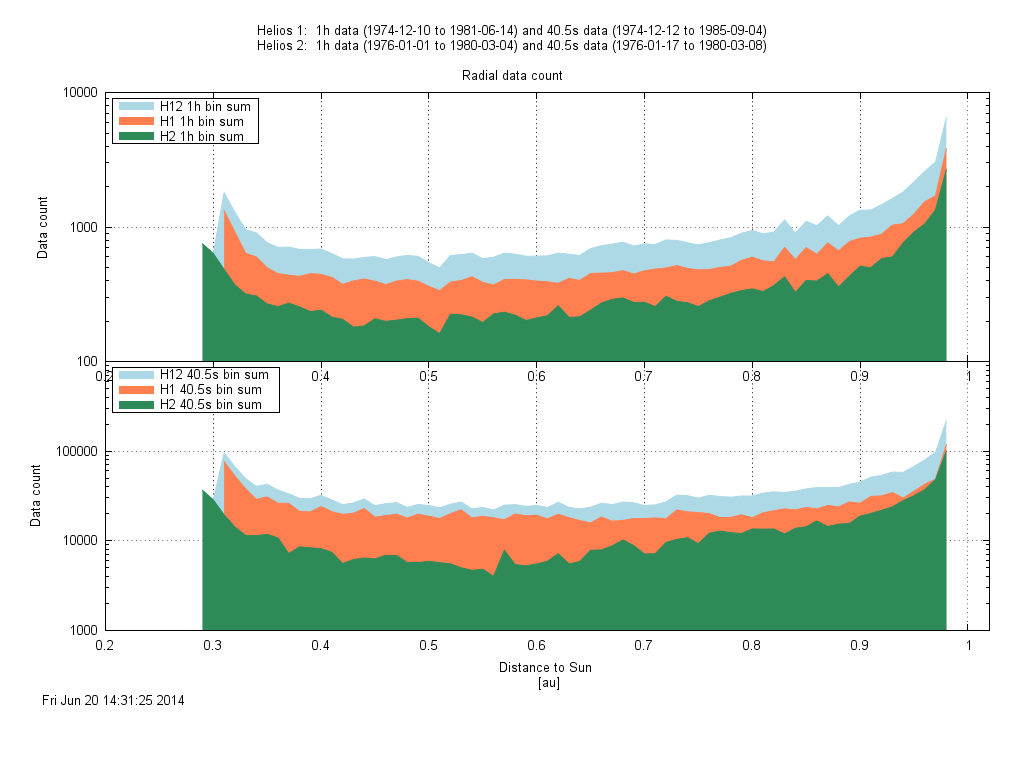
\includegraphics[width=0.45\textwidth]{images/gnuplots/Helios12_1h_magswe_r-count_plot.png}
		}{
			\caption{Plot of the Helios data count per 0.01~au solar distance bins. plot for mag and plasma individually..., combine with latitude plot...}
			\label{fig:Helios12_1h_magswe_r-count_plot}
		}
		\ffigbox{
			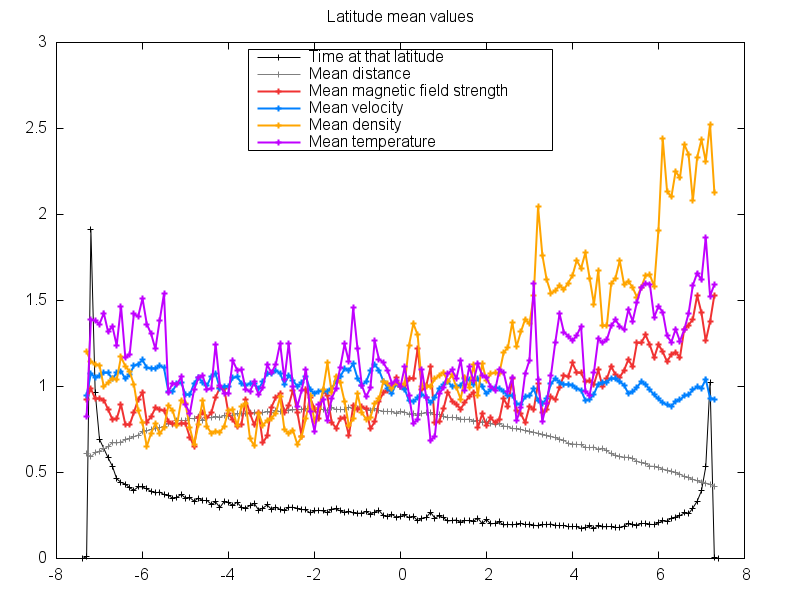
\includegraphics[width=\Xhsize]{images/gnuplots/latitude_frequency_plot.png}
		}{
			\caption{Plot of the Helios data count per 0.1° latitude. plot for mag and plasma individually... remove all other curves...}
			\label{fig:latitude_frequency_plot}
		}
	\end{floatrow}
\end{figure}

Solar wind data courtesy of R.~Schwenn, Max-Planck-Institut für Aeronomie, Lindau, magnetic field data courtesy of F.~Neubauer, Universität zu Köln. (see paper; into acknowledgements...)\\

%see presi 1.07 Inside Helios-Origins and Evolution-Salem.ppt
%see book Schwenn1990 https://books.google.de/books?id=W1DuCAAAQBAJ&printsec=frontcover&dq=Physics+of+the+Inner+Heliosphere+I.+Large-Scale+Phenomena&hl=de&sa=X&redir_esc=y#v=onepage&q=Physics%20of%20the%20Inner%20Heliosphere%20I.%20Large-Scale%20Phenomena&f=false



data sources -- see paper for replacing the following data\\
solar wind parameters: ACE, Helios, OMNI\\
geomagnetic indices: Kp, OMNI\\

Space Physics Data Facility (SPDF)\\

HELIOS 1 and 2 - orbital Parameters\\
\url{http://spdf.sci.gsfc.nasa.gov/pub/data/helios/helios1/traj/}\\
\url{http://spdf.sci.gsfc.nasa.gov/pub/data/helios/helios2/traj/}\\

Helios hourly merged mag \& plasma data:\\
HELIOS1\_COHO1HR\_MERGED\_MAG\_PLASMA\_2965.txt\\
HELIOS2\_COHO1HR\_MERGED\_MAG\_PLASMA\_3096.txt\\
\url{http://cdaweb.gsfc.nasa.gov}\\
temporal coverage of merged data\\
Helios 1: 1974-12-10 - 1981-06-14\\
Mag data availability: 42.6~\%\\
Plasma \& orbit data availability: 76.4~\%\\
Helios 2: 1976-01-01 - 1980-03-04\\
Mag data availability: 54.4~\%\\
Plasma \& orbit data availability: 91.8~\%\\

		%introduction, basics and data
%	\chapter{Data}
\label{chap:data}

	\chapter{Solar wind time variations}
\section{Solar wind variation with solar cycle}
\section{Solar wind variation with season}
\section{Solar wind empirical forecast}

\chapter{Solar wind distance variations}
\section{Solar wind back-extrapolation}


%COFI -- chapter outline and flow integration\\

see paper...\\

McGregor2011 analyzed the empirical magnetic topology–velocity relationship, using Helios perihelion data with the Wang-Sheeley-Arge (WSA) coronal model, and found indications, that the fast and slow solar wind are generated from distinct sources. (not only superradial expansion)\\


	\chapter{Helios radial line-up passings}

%COFI -- chapter outline and flow integration\\

have a look into Schwenn1984...\\

%motivation
To derive the radial dependence of the solar wind parameters directly, we look at the passings when both Helios spacecraft were radially lined up. In these cases they flew through the same solar wind at different solar distances.\\
(This eliminates the bias of averaging over slow and fast wind streams, like the described model does.)\\
see also \citet{Schwenn1990} p.~156 + p.~122...\\
%Helios line-up mapping techniques -> Schwenn1981 "Two states..." (not findable online after extensive search)

we compare these independently derived radial fit functions to those obtained from the averaging over all solar wind types...\\

%Helios passings, their time and position
There were eight passings when both Helios spacecraft were radially lined-up (see \autoref{fig:Helios12_lineup_positions_v3_pdfcairo_plot}).
\begin{figure}[htb]
	\centering
	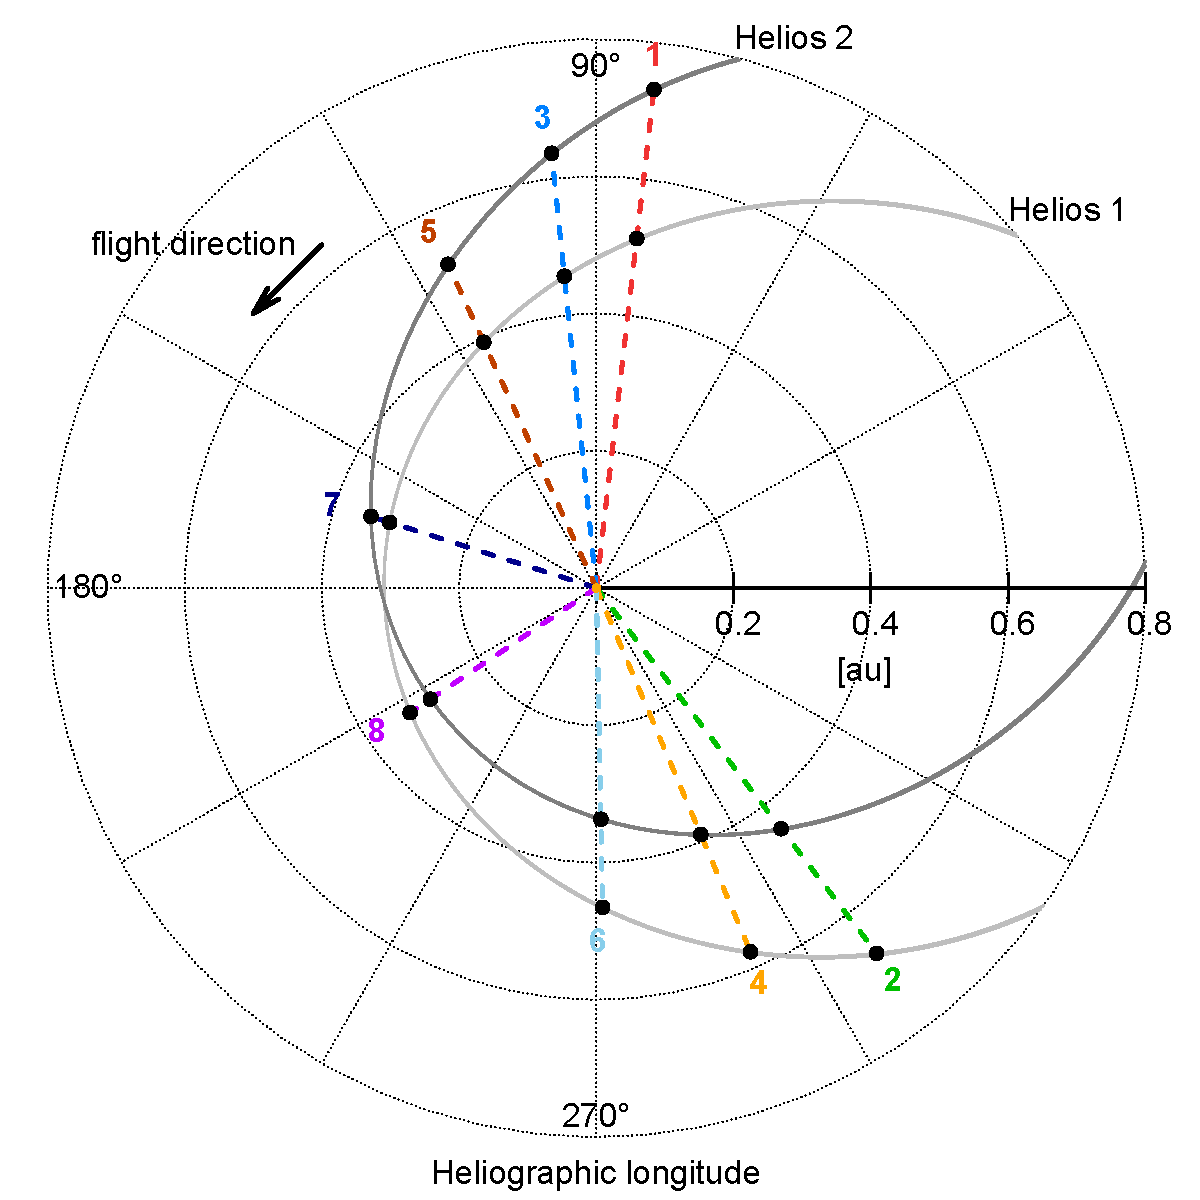
\includegraphics[width=0.6\textwidth]{images/gnuplots/Helios12_lineup_positions_v3_pdfcairo_plot.pdf}
	\caption{Schema of the eight spacecraft line-up positions of both Helios probes on their respective orbits. make B\&W... combine with fig 5.15? calibrate text size}
	\label{fig:Helios12_lineup_positions_v3_pdfcairo_plot}
\end{figure}
These points in time, when both probes had no separation in heliographic longitude, are derived from Helios~1 and Helios~2 daily trajectory data (for the data source see Section~XX). The data is linear interpolated to get an hourly resolution. The resulting points in time together with solar distances are listed in \autoref{tab:lineup_in_longitude}.
\begin{table}[htb]\small
	\centering
	\captionsetup{belowskip=4pt}
	\caption{Times when both Helios probes had no separation in heliographic longitude. Their solar distances (inner spacecraft $r_1$, outer spacecraft $r_2$) were in the range 0.291--0.731~au and the maximal inter-probe radial distance d$r$ was 0.229~au. errors in au...}
	\begin{tabular}{ccccccc}
		\toprule
		\multirow{2}{*}{Passing}	&\multirow{2}{*}{Date}	&\multirow{2}{*}{Time}	&\multirow{2}{*}{Inner s/c}	&$r_1$	&$r_2$	&d$r$\\
			&	&	&	&[au]	&[au]	&[au]\\
		\midrule
		1	&1976-03-09	&00:00	&Helios 1	&0.513	&0.731	&0.219\\
		2	&1976-05-02	&14:00	&Helios 2	&0.442	&0.671	&0.229\\
		3	&1976-09-19	&10:00	&Helios 1	&0.457	&0.637	&0.180\\
		4	&1976-10-31	&11:00	&Helios 2	&0.390	&0.576	&0.186\\
		5	&1977-04-02	&12:00	&Helios 1	&0.394	&0.519	&0.125\\
		6	&1977-04-30	&23:00	&Helios 2	&0.337	&0.465	&0.128\\
		7	&1977-10-18	&06:00	&Helios 1	&0.316	&0.345	&0.029\\
		8	&1977-10-25	&19:00	&Helios 2	&0.291	&0.327	&0.035\\
		\bottomrule
	\end{tabular}
	\label{tab:lineup_in_longitude}
\end{table}
%table data from
%file:///home/raid0/mvenzmer/Desktop/astro70/analyses/Helios12_1h_magswe/Helios12_1h_inline/lineup_periods_v3.txt

%excluding period 7 and 8
The last two passings were merely one week apart and the Helios probes flew almost without radial separation because Helios~2 overtook Helios~1 during its perihelion. As we want to analyze the same solar wind at different solar distances, we exclude the passings 7 and 8 from further analyses.\\


%defining line-up requirements
The passing longitude is not the same as the longitude where the solar wind is detected by both spacecraft consecutively. A passing occurs shortly before the points in time when both spacecraft observe the same solar wind. For the outer probe this point in time is shifted by the solar wind's travel time. The travel time depends on the solar wind's velocity and its distance traveled.\\


%calculation of the offset times
Based on the obtained spacecraft line-up time $t_0$ one can calculate the offset times $t_1$ and $t_2$ when the inner and outer spacecraft pass by the same solar wind (see \autoref{fig:Helios12_lineup_calculation_pdfcairo_plot}). At the solar wind line-up longitude the condition
\begin{align}
	t_2 = t_1 + t_\text{sw} \label{eq:lineup_condition}
\end{align}
holds. As the offset times depend on the solar wind travel time between the probes, we need knowledge of the solar wind velocity $v$ for their calculation: $t_\text{sw} = \text{d}r/v$, with the mean radial separation distance d$r$ between the probes.
\begin{figure}[htb]
	\centering
	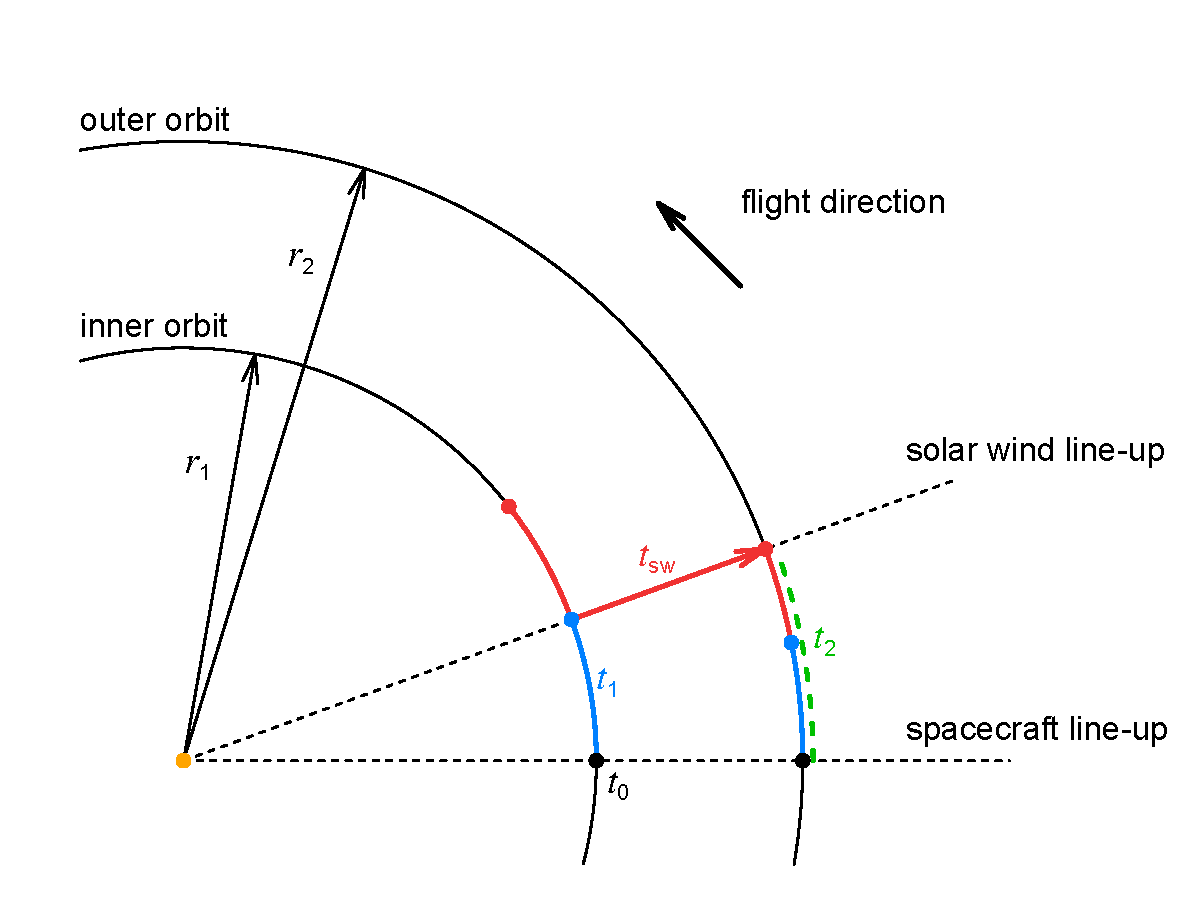
\includegraphics[width=0.5\textwidth]{images/gnuplots/Helios12_lineup_calculation_pdfcairo_plot.pdf}
	\caption{Illustration of the solar wind line-up longitude situation with the spacecraft line-up time $t_0$, the offset times $t_1$, $t_2$ (at which the spacecraft measure the same solar wind) and the solar wind travel time $t_\text{sw}$. combine with fig 5.14?}
	\label{fig:Helios12_lineup_calculation_pdfcairo_plot}
\end{figure}
%/home/raid0/mvenzmer/Desktop/astro70/analyses/Helios12_1h_magswe/Helios12_1h_inline/Helios12_lineup_calculation_pdfcairo_gps.txt

%calculating t_1
For the calculation of $t_1$ we recall the third Kepler law
\begin{align}
	\frac{{T_1}^2}{{T_2}^2} = \frac{{a_1}^3}{{a_2}^3}
\end{align}
with the orbital periods $T_1$, $T_2$ and the semi-major axes $a_1$, $a_2$. The assumption of circular orbits (why? what error size?) leads to
\begin{align}
	\frac{{t_1}^2}{(t_1 + t_\text{sw})^2} &= \frac{{r_1}^3}{{r_2}^3}	\nonumber\\
	\Leftrightarrow\qquad\qquad	t_1 &= t_\text{sw} \left( \left( \frac{r_1}{r_2} \right)^\frac{3}{2} - 1 \right)^{-1} \label{eq:offset_time}
\end{align}
and finally the offset time $t_1$ only depends on the variable solar wind travel time $t_\text{sw}$.\\

%calculating the offset time from the solar wind velocity
Due to uncertainties in the travel time $t_\text{sw}$ (the solar wind speed $v$ is obviously not a constant) the exact calculation of $t_1$ is imprecise. To get a reliable result we perform two iterations calculating the offset time from the average velocity $\bar{v}$ of the surrounding 2-day period. We use the velocity $\bar{v}_0$ around $t_0$ to calculate the offset time $t'_1$ as a first estimate. As the velocity $\bar{v}'_1$ at $t'_1$ is certainly different, we use this velocity to refine the value and obtain $t_1$. Hence deriving the velocity $\bar{v}_1$ enables us to calculate the solar wind travel time $t_\text{sw}$.

%We have to round the offset times and time shift values to full hours, because we use the hourly merged mag and plasma Helios data set (see Section~XX) for the velocity calculation.
The average velocities are obtained from the hourly merged (mag?) and (plasma?) Helios data set (see Section~XX). The resulting offset times and velocities of both iterations together with the travel times are listed in \autoref{tab:offset_times}.
\begin{table}[htb]\small
	\centering
	\captionsetup{belowskip=4pt}
	\caption{The two iterations of the derived offset times and average velocities. The resulting solar wind travel times have durations of 11--28~hours. errors...}
	\begin{tabular}{cccccccc}
		\toprule
		\multirow{2}{*}{Passing}	&\multirow{2}{*}{Inner s/c}	&$v_0$	&$t'_1$	&$v'_1$	&$t_1$	&$v_1$	&$t_\text{sw}$\\
			&	&[km/s]	&[h]	&[km/s]	&[h]	&[km/s]	&[h]\\
		\midrule
		1	&Helios 1	&659.3	&19.6	&656.9	&19.7	&656.9	&13.9\\
		2	&Helios 2	&436.4	&25.1	&370.9	&29.5	&356.7	&26.7\\
		3	&Helios 1	&482.6	&24.0	&444.0	&26.1	&413.8	&18.1\\
		4	&Helios 2	&302.3	&32.2	&279.9	&34.8	&278.3	&27.8\\
		5	&Helios 1	&507.3	&20.0	&474.8	&21.4	&473.5	&11.0\\
		6	&Helios 2	&321.2	&26.6	&392.6	&21.7	&367.8	&14.5\\
		\bottomrule
	\end{tabular}
	\label{tab:offset_times}
\end{table}
%table data from
%file:///home/raid0/mvenzmer/Desktop/astro70/analyses/Helios12_1h_magswe/Helios12_1h_inline/lineup_periods_v3.txt

%introducing the lag time for arbitrary longitude positions
For the solar wind line-up longitude condition~\eqref{eq:lineup_condition} holds. For all other positions the solar wind measured by the inner spacecraft will not arrive the outer orbit position at the same time as the outer spacecraft does (see \autoref{fig:Helios12_lineup_calculation_delay_pdfcairo_plot}).
\begin{figure}[htb]
	\centering
	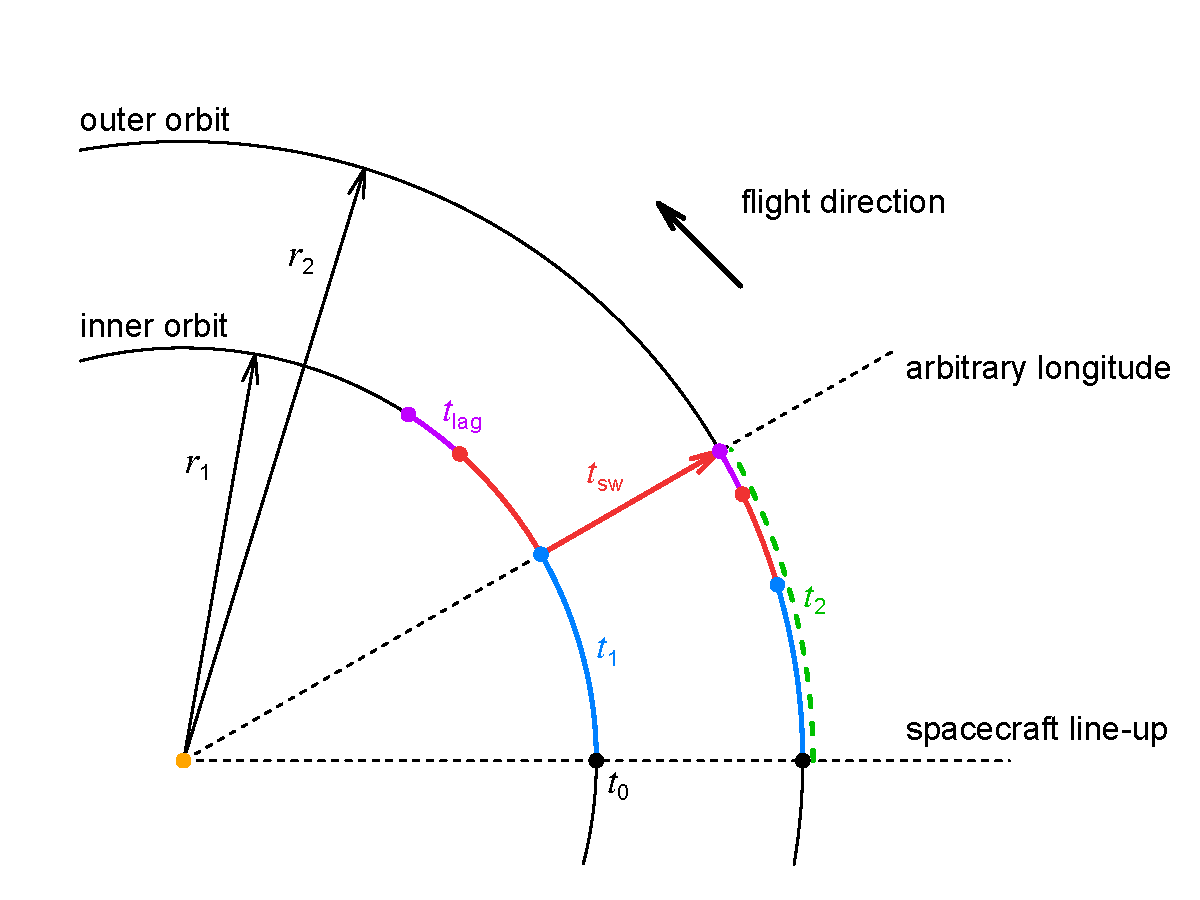
\includegraphics[width=0.5\textwidth]{images/gnuplots/Helios12_lineup_calculation_delay_pdfcairo_plot.pdf}
	\caption{Illustration like \autoref{fig:Helios12_lineup_calculation_pdfcairo_plot} but for arbitrary longitude situations a lag time $t_\text{lag}$ comes into play. merge with fig 5.14?}
	\label{fig:Helios12_lineup_calculation_delay_pdfcairo_plot}
\end{figure}
%/home/raid0/mvenzmer/Desktop/astro70/analyses/Helios12_1h_magswe/Helios12_1h_inline/Helios12_lineup_calculation_delay_pdfcairo_gps.txt

Either the spacecraft (negative lag time) or the solar wind (positive lag time) already have passed this position:
\begin{align}
	t_2 = t_1 + t_\text{sw} + t_\text{lag}. \label{eq:lag_time}
\end{align}
This lag time $t_\text{lag}$ is the time difference at which the solar wind is probed by both spacecraft. At the spacecraft line-up longitude ($t_1 = t_2 = 0$) the lag time equals the solar wind travel time and at the solar wind line-up longitude the lag time is zero.\\

%calculation of the +-24 hour solar wind time span
We choose to look at time periods (instead of points in time) around the offset times to derive average solar wind parameters. This helps reducing the influence of solar wind fluctuations.\\

We define the period duration boundaries as when the lag time $t_\text{lag}$ is in the range $\pm24$~h. For the outer spacecraft these periods are almost twice as long as for the inner spacecraft. The calculated period start and end hours (relative to $t_0$) for both spacecraft are listed in \autoref{tab:period_times_coverage} together with the data coverage of these periods.
\begin{table}[htb]\small
	\centering
	\captionsetup{belowskip=4pt}
	\caption{Derived period start and end hours for both spacecraft in relation to the longitude line-up time $t_0$. The corresponding combined data coverage within that period of the magnetic field, velocity, density and temperature is listed as well. instead duration! errors...}
	\begin{tabular}{cccrrccrrc}
		\toprule
		\multirow{3}{*}{Period}	&	&\multicolumn{4}{c}{Inner spacecraft}	&	&\multicolumn{3}{c}{Outer spacecraft}\\
		\cmidrule{3-6}	\cmidrule{8-10}
			&	&\multirow{2}{*}{s/c}	&Start	&End	&Coverage	&	&Start	&End	&Coverage\\
			&	&	&[h]	&[h]	&[\%]	&	&[h]	&[h]	&[\%]\\
		\midrule
		1	&	&Helios 1	&-14.4	&53.8	&73	&	&-24.6	&91.6	&99\\
		2	&	&Helios 2	&3.1	&58.3	&89	&	&5.8	&109.0	&88\\
		3	&	&Helios 1	&-9.2	&65.1	&16	&	&-15.1	&107.2	&10\\
		4	&	&Helios 2	&4.8	&65.2	&59	&	&8.5	&117.0	&87\\
		5	&	&Helios 1	&-25.5	&68.3	&89	&	&-38.5	&103.3	&88\\
		6	&	&Helios 2	&-15.3	&61.7	&93	&	&-24.8	&100.1	&92\\
		\bottomrule
	\end{tabular}
	\label{tab:period_times_coverage}
\end{table}
% %table data from
% %file:///home/raid0/mvenzmer/Desktop/astro70/analyses/Helios12_1h_magswe/Helios12_1h_inline/lineup_periods_v3.txt

%excluding period 3
For period~3 the combined data coverage of the four solar wind parameters is only 16~\% (Helios~1) and 10~\% (Helios~2) respectively. We consider this as insufficient for the continuing analysis and therefore also omit period~3.\\

The five remaining periods are marked in \autoref{fig:Helios12_lineup_period_positions_v3_pdfcairo_plot}.
\begin{figure}[htb]
	\centering
	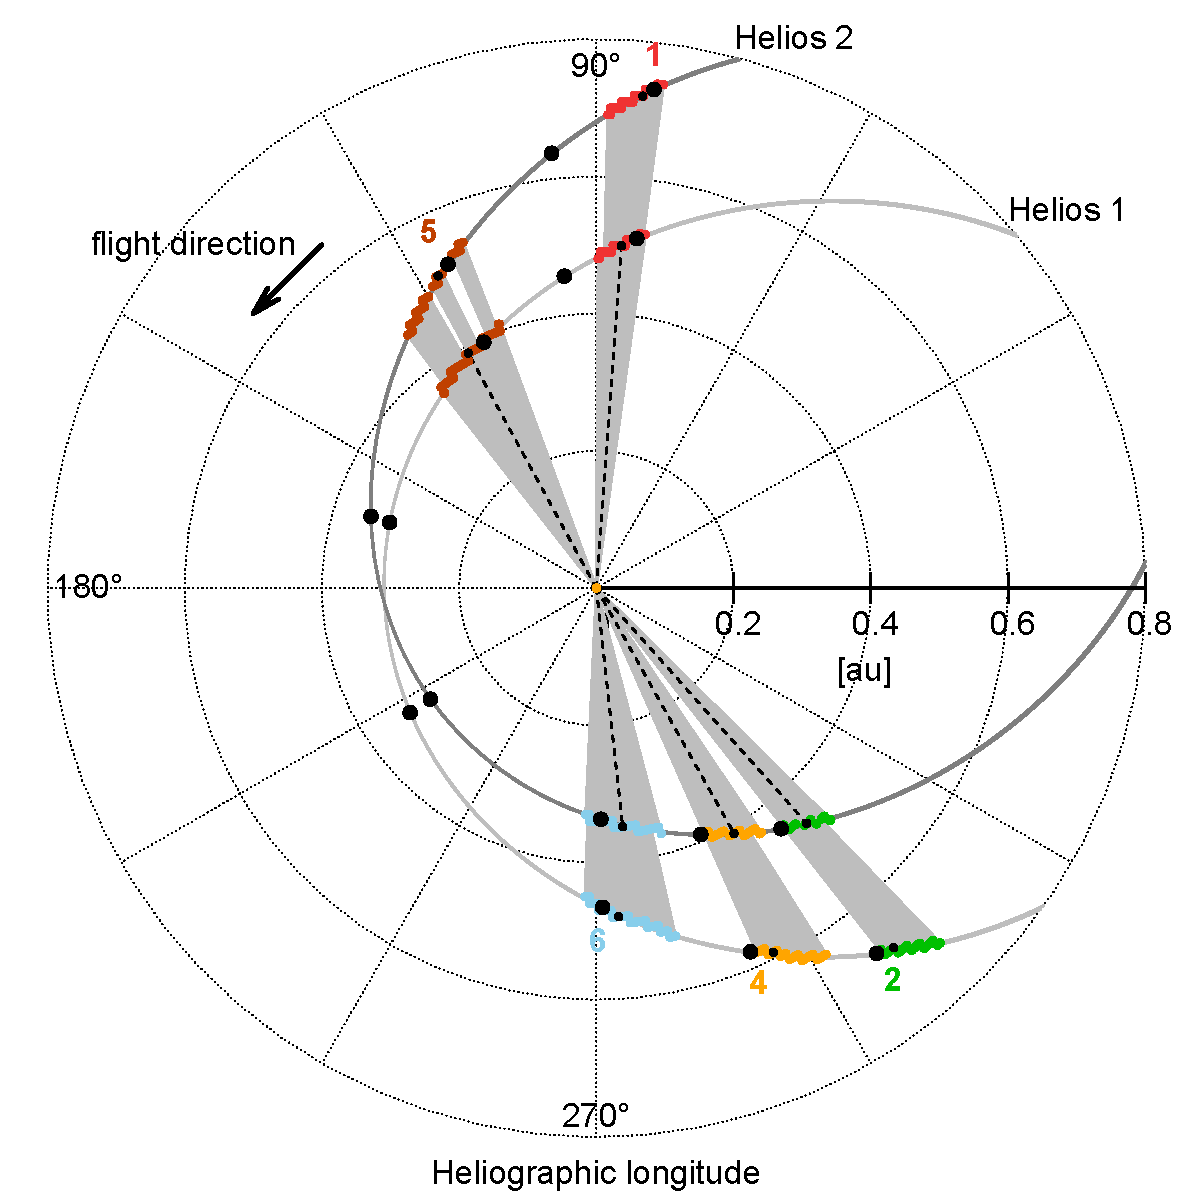
\includegraphics[width=0.6\textwidth]{images/gnuplots/Helios12_lineup_period_positions_v3_pdfcairo_plot.pdf}
	\caption{Scheme of the line-up periods of both Helios spacecraft on their respective orbits. The corresponding orbit sections which we consider in our analysis are marked in color. These sections span the positions where both spacecraft observed the same solar wind with a maximal lag time of $\pm24$~hours. bw figure?? dotted lines?}
	\label{fig:Helios12_lineup_period_positions_v3_pdfcairo_plot}
\end{figure}

%average values
The average values of the four parameters magnetic field $B$, velocity $v$, density $n$ and temperature $T$ are listed in \autoref{tab:period_means}.
\begin{table}[htb]\small
	\centering
	\captionsetup{belowskip=4pt}
	\caption{Average values of the four solar wind parameters magnetic field, velocity, density and temperature for the individual periods and spacecraft. errors...}
	\begin{tabular}{cccrrrrcrrrr}
		\toprule
		\multirow{3}{*}{Period}	&	&\multicolumn{5}{c}{Inner spacecraft}	&	&\multicolumn{4}{c}{Outer spacecraft}\\
		\cmidrule{3-7}	\cmidrule{9-12}
			&	&\multirow{2}{*}{s/c}	&\multicolumn{1}{c}{$B$}	&\multicolumn{1}{c}{$v$}	&\multicolumn{1}{c}{$n$}	&\multicolumn{1}{c}{$T$}	&	&$B$	&$v$	&$n$	&$T$\\
			&	&	&\multicolumn{1}{c}{[nT]}	&\multicolumn{1}{c}{[km/s]}	&\multicolumn{1}{c}{[cm$^{-3}$]}	&\multicolumn{1}{c}{[K]}	&	&[nT]	&[km/s]	&[cm$^{-3}$]	&[K]\\
		\midrule
		1	&	&Helios 1	&17.04	&646.4	&12.0	&367\,300	&	&8.93	&602.8	&6.7	&244\,000\\
		2	&	&Helios 2	&15.77	&356.4	&38.8	&122\,400	&	&12.05	&390.2	&17.7	&117\,200\\
		4	&	&Helios 2	&15.18	&281.3	&108.0	&46\,000	&	&10.64	&298.6	&46.1	&30\,400\\
		5	&	&Helios 1	&28.80	&521.3	&45.9	&337\,800	&	&18.73	&530.3	&24.4	&282\,000\\
		6	&	&Helios 2	&29.57	&402.4	&82.5	&271\,900	&	&14.71	&432.6	&35.7	&199\,100\\
		\bottomrule
	\end{tabular}
	\label{tab:period_means}
\end{table}
%table data from
%file:///home/raid0/mvenzmer/Desktop/astro70/analyses/Helios12_1h_magswe/Helios12_1h_inline/lineup_periods_v3.txt

%solar wind feature match
If we compare both, the inner solar wind sections together with their outer counterparts, they indeed appear to have a similar shape apart from the time shift (see \autoref{fig:Helios12_lineup_period_1_7d_v3_plot}) (name definite features...). This confirmes that they indeed are parts of the same solar wind structures.\\
maybe figures of all into Appendix?...\\
\begin{figure}[htb]
	\centering
	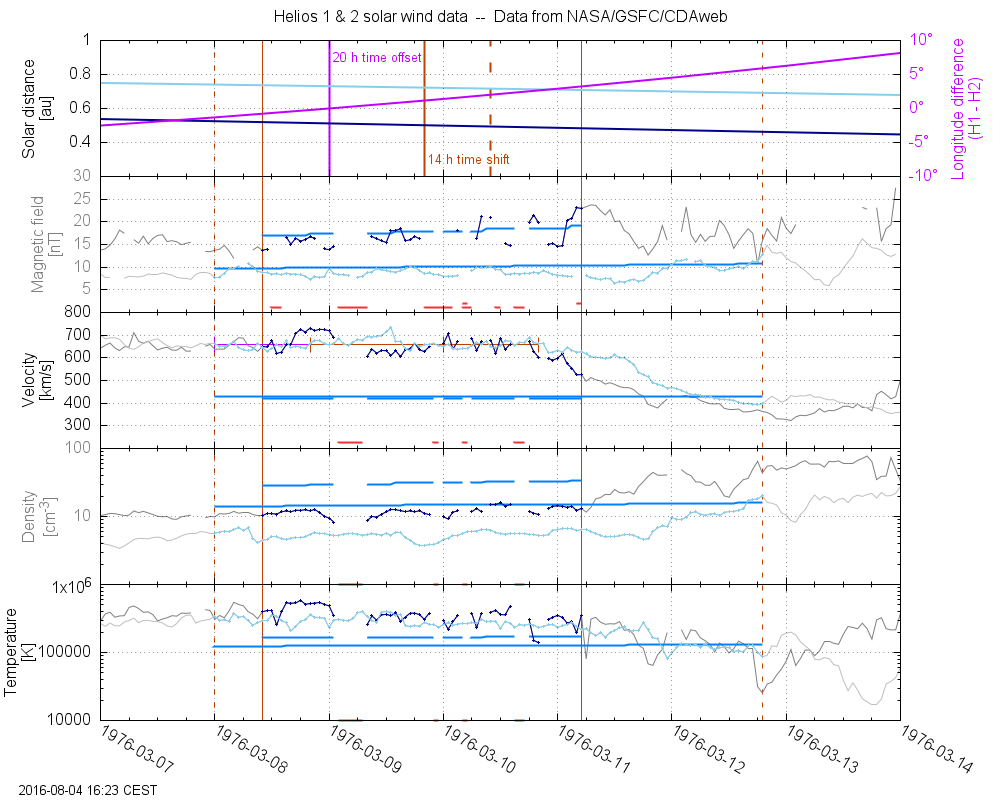
\includegraphics[width=0.5\textwidth]{images/gnuplots/Helios12_lineup_period_1_7d_v3_plot.png}
	\caption{Measured solar wind parameters $B$, $v$, $n$, and $T$ of both spacecraft in the period~1. Also plotted is the spacecraft's separation in heliographic longitude. offset time, time shift; expected value from the radial sw model... remove date... remove solar distance... adjust text size...}
	\label{fig:Helios12_lineup_period_1_7d_v3_plot}
\end{figure}


%solar wind types
the comparison to the sw model's mean value at the individual distances lets us classify the solar wind types...
\begin{description*}
	\item[Period 1]	HSS
	\item[Period 2]	medium--LSS
	\item[Period 4]	LSS
	\item[Period 5]	medium--HSS
	\item[Period 6]	LSS--HSS
\end{description*}

%...forward- and back-matching data gaps results in worse data coverage!

%fit function parameters
We obtained the mean parameter values for the inner and outer solar wind sections. As with the overall radial dependency before, these two points are fitted to the exponential regression fit function $X(r) = X_0\,r^{c_X}$ (see Section~XX. The resulting fit coefficients for each period are listed in \autoref{tab:lineup_fit_functions}.\\
why is it better to fit the period's mean values than the whole period?...\\
we fit the periods' mean value rather than the whole periods, because...\\

\begin{table}[htb]\small
	\centering
	\captionsetup{belowskip=4pt}
	\caption{Radial fit functions $B(r)$, $v(r)$, $n(r)$ and $T(r)$ for each period. or only the variables into table? error sizes...}
	\begin{tabular}{cgggg}
		\toprule
		\multirow{2}{*}{Period}	&B(r) =,B_0~r^{c_B}	&v(r) =,v_0~r^{c_v}	&n(r) =,n_0~r^{c_n}	&T(r) =,T_0~r^{c_T}\\
			&\text{[nT]},	&\text{[km/s]},	&\text{[cm$^{-3}$]},	&\text{[K]},\\
		\midrule
		1	&4.88,r^{-1.815}	&564.7,r^{-0.196}	&3.9,r^{-1.647}	&166\,500,r^{-1.148}\\
		2	&9.50,r^{-0.654}	&442.6,r^{0.220}	&8.9,r^{-1.902}	&112\,800,r^{-0.106}\\
		4	&6.79,r^{-0.900}	&322.0,r^{0.151}	&15.7,r^{-2.155}	&18\,000,r^{-1.047}\\
		5	&5.99,r^{-1.649}	&554.8,r^{0.065}	&4.6,r^{-2.423}	&174\,700,r^{-0.692}\\
		6	&3.22,r^{-2.108}	&506.5,r^{0.219}	&5.7,r^{-2.533}	&101\,000,r^{-0.941}\\
		\midrule
		weigthed by duration mean functions\\
		\midrule
		mean of sw model (update)	&6.078,r^{-1.563}	&435.5,r^{0.04955}	&7.613,r^{-2.032}	&97\,050,r^{-0.8002}\\
		\bottomrule
	\end{tabular}
	\label{tab:lineup_fit_functions}
\end{table}
%table data from
%file:///home/raid0/mvenzmer/Desktop/astro70/analyses/Helios12_1h_magswe/Helios12_1h_inline/lineup_periods_v3.txt

%interpretation
The fit curves show noticeable deviations from the model's mean fit (see \autoref{fig:Helios12_lineup_fit_Bmean_v3_final_plot}). maybe 4-panel figure?; maybe figures of all into Appendix?\\
\begin{figure}[htb]
	\centering
	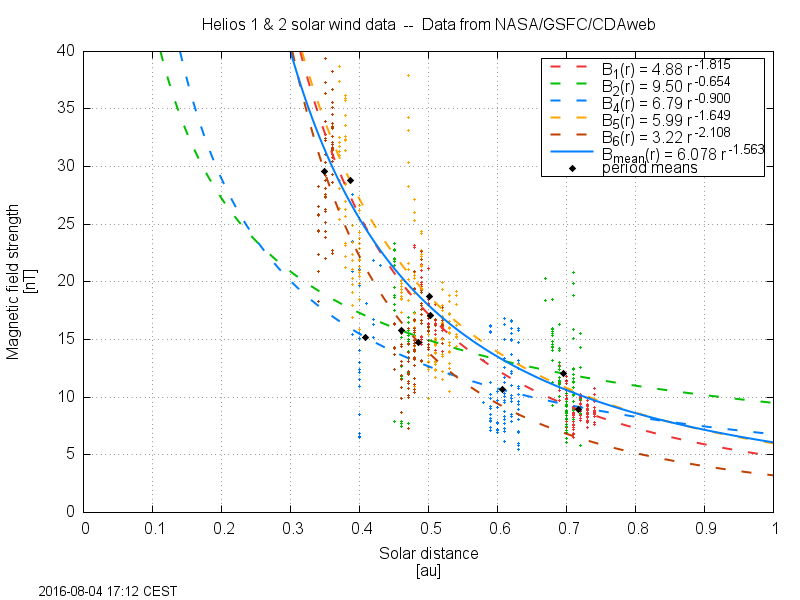
\includegraphics[width=0.5\textwidth]{images/gnuplots/Helios12_lineup_fit_Bmean_v3_final_plot.png}
	\caption{Fit curves of the radial magnetic field. The fits are based on the mean values (meanr,meanB; black points) of the line-up periods. build pdf figure... remove date... adjust text size... 4-figure?}
	\label{fig:Helios12_lineup_fit_Bmean_v3_final_plot}
\end{figure}
The observed deviations are as expected from these types of solar wind. ...are they? analyze each in detail...\\
argue from sw type; slow, medium and fast type; check their position relative to the mean curve...\\

%what we have learned
results:\\
features of calculated line-up periods match.\\
their derived fit functions scatter within (acceptable?) margin around model's radial mean, backing its applicability.\\



	\chapter{Solar wind impact on the magnetosphere}
%\label{chap:}

motivation (see also introduction): solar wind impact nowcast, CME impact forecast\\
%COFI -- chapter outline and flow integration\\


\section{Solar wind interaction processes with the magnetosphere}
%\label{sec:}

%theory
As is known for some time the terrestrial magnetic field shows disturbances that are caused by solar wind (see \autoref{sec:solar_influence_on_earth}).\\

there are several underlying physical mechanisms, whose contribution is not yet quantified'?'\\
% physical mechanisms:\\
% - reconnection\\
% - compression\\
% - turbulence\\
% - induction?\\

three ways for solar wind momentum and energy transfer into magnetosphere:\\
- sw entering sphere\\
- waves/eddies\\
- reconnection\\

%[the relation of these events was confirmed two decades ago by (who and \citet{Bothmer1993})]\\

-> example events CIR/HSS and CME\\


\section{Solar wind--magnetosphere coupling functions}
\label{sec:solar_wind_magnetosphere_coupling_functions}

%theory from literature
coupling mechanisms and therefrom derived functions\\
VBzgsm - E-field...\\

Studies finding best coupling function, Newell, etc.\\

\citet{Newell2007}: universal sw-magnetosphere coupling function (opening flux rate)\\
\citet{Newell2008}: coupling function merging and viscous term\\
merging and viscous terms (reconnection and turbulence)\\
merging term: rate magnetic flux is opened at the magnetopause ($d\Phi_\text{MP}/dt$)\\
viscous term: reconnection due to Kelvin-Helmholtz instabilies at the boundary ($n^{1/2} v^2$)\\
equation for the least variance linear prediction of Kp: $Kp = 0.05 + \num{2.244e-4} d\Phi_\text{MP}/dt + \num{2.844e-6} n^{1/2} v^2$\\
combination of both terms works best (r = 0.866)\\

see also \autoref{sec:solar_wind_magnetosphere_coupling}\\


\section{Parameter selection}

%fix usage of Kp index\\
In our analyses we use the planetary geomagnetic disturbance indicator Kp (see Section~XX...), because it is designed to measure solar particle radiation by its magnetic effects (cite? Bartels...?).\\
and close relation to aurorae, NOAA scale\\

choose solar wind parameters based on coupling functions\\
V, B, Bzgsm, N, T\\


\section{Data selection}

choose data sets, data resolution and time period\\

geomagnetic disturbance index Kp: magnetic field maximal variation range within 3~hours; 3-hourly index\\
need high resolution solar wind data (e.g. 1~min) to be able to determine maximal values/variations within 3~hours\\

choosing data time range\\
the Kp time series started in XXXX, when there were no spacecraft to measure in situ solar wind --> time range defined by available solar wind data\\
OMNI data set -> longest continuous solar wind data set\\


data processing\\
choosing data averaging duration and method (min/avg/max)\\
OMNI 1min data to 3hmin/max\\
now: 3~hour solar wind extreme value, to back up argument refer to cc table (same data period, different resolution/measure (measure=mean, max or min))\\
		(tested: 3"~hour solar wind variation range gives 8~\% lower cc)\\


\section{General Kp correlations}

general frequency distributions\\

general correlation coefficients + plots\\

general cc table\\

\section{Solar cycle influence}

solar cycle dependence\\
- parameter time plots\\
- parameter vs SSN matrix-plots\\
- cc time plots\\
- cc vs SSN plots\\

\section{Isolating the CME influence}

the causes of the strongest geomagnetic storms are draping and magnetic clouds of CMEs \citep{Bothmer1993}\\

-> example event CME\\

\subsection{Solar wind structure list}

solar wind structures (SWS) OMNI list of Ian~Richardson \citep{Richardson2012}\\
open source 1995--2015 \url{http://www.srl.caltech.edu/ACE/ASC/DATA/level3/icmetable2.htm}\\
restricted source 1963--2015 \url{http://cedarweb.vsp.ucar.edu/wiki/index.php/Tools_and_Models:Solar_Wind_Structures} \citet{Richardson2012}\\	%Rules of the Road: Please contact Ian Richardson about your use of this data.

overall CME fraction of solar wind - compute (for used period) from file $sws_swstruc_yearly_63001_14035.txt$\\
e.g. 2013: 0.220 CMEs, 0.236 CIRs/HSSs and 0.544 slows (low speed streams - LSSs)\\

\subsection{CME correlations}

same analysis for CMEs\\
- parameter time plots\\
- parameter vs SSN matrix-plots\\
- cc time plots\\
- cc vs SSN plots\\


	
\chapter{Solar wind impact on the terrestrial magnetosphere}
%\chapter{}

% Alle Presis ausschlachten!
% Alle Projektberichte ausschlachten!
% Kp8--Liste irgendwo einweben...
% paper draft 2014 ausschlachten...

%Questions addressed in this thesis
Questions:\\
	How strong is the solar wind influence on the terrestrial magnetosphere?\\
	How strong do different structure types influence the terrestrial magnetosphere?\\
	
	How can the impact strength of the solar wind be forecasted? (VBz->Kp L1-Alerts)\\
	How can the impact strength of CMEs be forecasted (V->Kp correlation for CMEs)?\\
	(How can the impact field strength of CMEs be forecasted (V->B correlation for CMEs)?)\\


%On solar wind acceleration and SPP proposition: McComas2007


% Analyses structure:\\
% 
% Core studies:
% Motivational question: Which solar wind structures contribute to the individual Kp ranges?
% define OMNI data set duration
% build Kp histogram
% 	for each Kp range
% 		extract contributing solar wind sections
% 			get sections structure flag
% 		derive individual structure contribution
% 
% preparations:
% analyze solar wind and categorize its structure types
% 	define thresholds for event recognition
% 	write automatic event recognition program
% 	=> flagged time series
% 	(additional output: OMNI solar wind event list)
% 
% applications:
% - Kp nowcast with L1 solar wind measurements (L1 alerts, disseminated as RSS feeds; integrated in smartphone app and space weather display)
% - Forecast of the possible CME impact on the Earths magnetosphere (Kp index) from the predicted CME arrival velocity (integrated in UGOE CME forecast chain (aka DDC))
% 
% 
% Further studies:
% Motivational question: What is the evolution of the solar wind parameters/structures before arriving at Earth? %what is meant by the term evolution?
% define Helios data set
% extrapolation of the solar wind parameters with the use of regression fitting
% extraction of distance independent time series with regression fits
% get flagged time series from distance independent time series
% (like before:)
% analyze solar wind and categorize its structure types
% 	define thresholds for event recognition
% 	write automatic event recognition program
% 	=> flagged time series
% 	(additional output: Helios solar wind event list)
% 
% 
% empirical radial solar wind model:
% derive the characteristic distributions of the solar wind parameters from OMNI data
% combination of the OMNI characteristic distributions with the Helios extrapolation
% 	(additional output: empirical radial probability distribution model)
% 
% Applications:
% - The near-sun* solar wind extrapolation can be useful for the planned Solar Probe Plus mission


\section{Quantifying solar wind impact on the terrestrial magnetosphere}
%\label{sec:}

linear velocity replacement of ACE realtime data with Kp, Machol2013\\

3hmin(vBzgsm) performs in rank correlation slightly better than the sophisticated Newell formula\\

%How strong does the solar wind influence the terrestrial magnetosphere?\\
[To quantify this we correlate terrestrial magnetic field measurements with in situ solar wind measurements.]\\


analyze sw coupling to the magnetosphere (Kp)\\
coupling functions\\

choosing data sets:\\
	% sw data OMNI 1h and 1min comparison\\
	% 1h3hmin vs 1min3hmin correlation\\

choosing solar wind parameters\\
	comparison of their correlation coefficients in table...\\
		-> Pearson or Spearman rank cc?? (Appendix?)\\
		-> lag meaning?\\
	% bulk correlation coefficients and functions\\
	% B-Kp, V-Kp, Bz-Kp
	
What kind of correlation function with these parameters?\\
% comparison with existing solar wind-magnetosphere coupling functions (see Basics chapter)\\


comparison of correlation coefficients for different data resolutions and measures in \autoref{tab:cc_measure_comparison}.
\begin{table}[htb]\small
	\centering
	\captionsetup{belowskip=4pt}
	\caption{Pearson correlation coefficients of Kp with sample solar wind parameters for different data resolutions and measures for comparison. 3h 1min extrema data results in slightly higher ccs... (use Spearman instead?)}
	\begin{tabular}{lcccc}
		\toprule
			&OMNI 1h	&OMNI 1h	&OMNI 1min	&OMNI 1min\\
			&1963-201308	&1963-201308	&19850101-20150101	&19850101-20150101\\
			&3h mean	&3h 1h extrema	&3h 10min extrema	&3h 1min extrema\\
		\midrule
		V	&0.568	&0.579	&?	&0.598\\
		B	&	&	&	&\\
		\bottomrule
	\end{tabular}
	\label{tab:cc_measure_comparison}
\end{table}


correlation coefficients in \autoref{tab:correlation_coefficients}.
\begin{table}[htb]\small
	\centering
	\captionsetup{belowskip=4pt}
	\caption{Pearson correlation coefficients of Kp with solar wind parameters... (use Spearman instead?)}
	\begin{tabular}{cc}
		\toprule
			&OMNI 1min\\
		Parameter	&19850101-20150101\\
			&3h 1min max\\
		\midrule
		N	&0.199792\\
		V	&0.598351\\
		T	&0.510607\\
		B	&0.595860\\
		Bzgsm	&-0.666050$^\text{a}$\\
		V*B	&0.682383\\
		V*Bzgsm	&-0.715101$^\text{a}$\\
		N*T	&\\
		\bottomrule
		\multicolumn{2}{l}{\footnotesize{$^\text{a}$Here it is min instead of max.}}
	\end{tabular}
	\label{tab:correlation_coefficients}
\end{table}


resulting figure VBzgsmvsKp; candle flame shape\\
see \autoref{fig:2Dhistogram_3hmin_VBzgsmvsKp_new_plot}
\begin{figure}[htb]
	\centering
	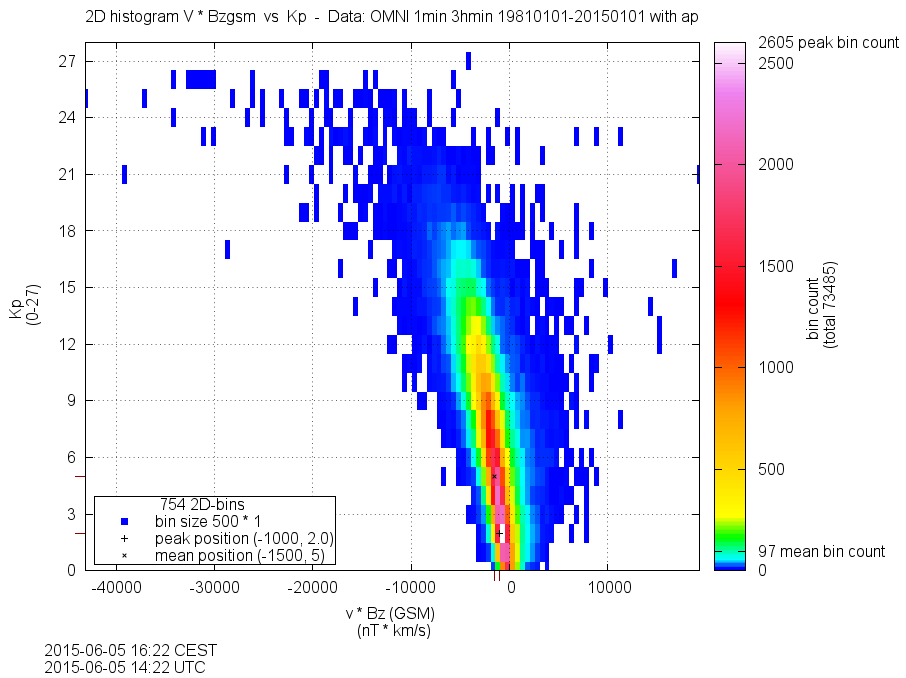
\includegraphics[width=0.3\textwidth]{images/gnuplots/2Dhistogram_3hmin_VBzgsmvsKp_new_plot.png}
	\caption{Plot fo Kp frequency by V*Bzgsm. make plot flatter...}
	\label{fig:2Dhistogram_3hmin_VBzgsmvsKp_new_plot}
\end{figure}

correlation coefficient...\\

VBzgsmvsKp dependence plot; V shape\\
see \autoref{fig:2Dhistogram_3hmin_VBzgsmvsKp_new_dependence_plot}
\begin{figure}[htb]
	\centering
	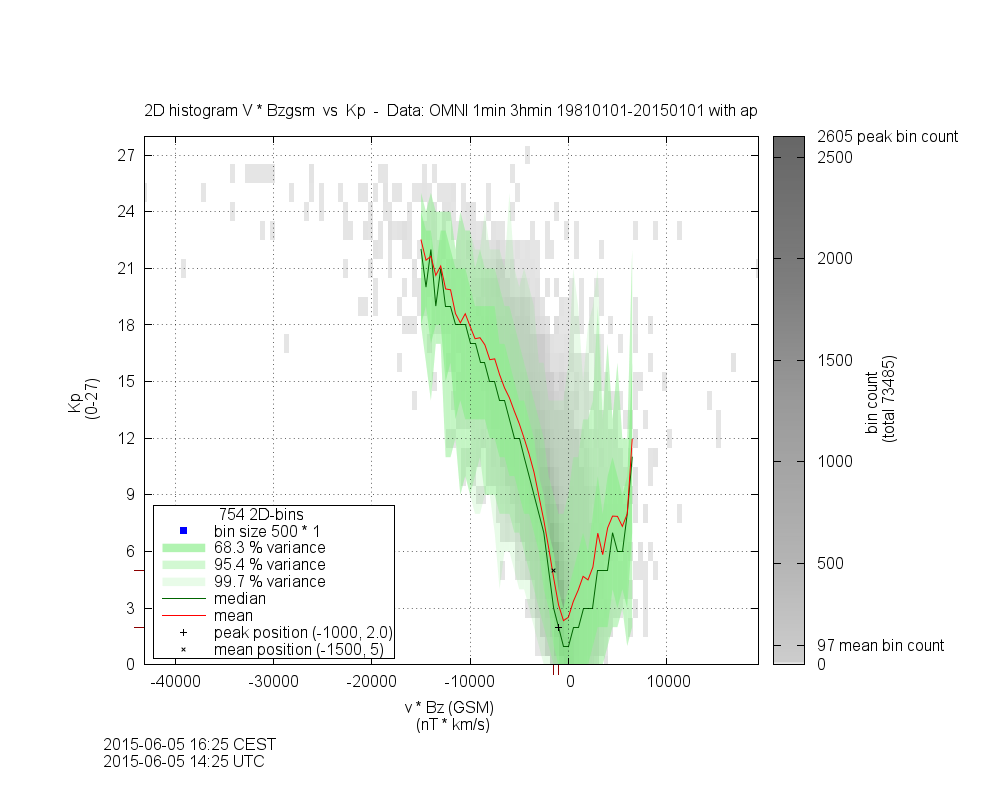
\includegraphics[width=0.3\textwidth]{images/gnuplots/2Dhistogram_3hmin_VBzgsmvsKp_new_dependence_plot.png}
	\caption{Plot like Figure~XX but with the Kp dependency.}
	\label{fig:2Dhistogram_3hmin_VBzgsmvsKp_new_dependence_plot}
\end{figure}

Results of this section.\\
What kind of solar wind structures create the individual regions in this distribution? -> next section\\
What is their individual contribution to the Kp ranges (e.g. high Kp: CMEs 70\% and CIRs 30\%)? -> next section\\

maybe correlation coefficient frequency spectra over time...?\\


\section{Solar wind structure type influence on the terrestrial magnetosphere}

How strong do different structure types influence the terrestrial magnetosphere?\\

present single events, avg solar wind and CME\\
show for both VBzgsmvsKp plot

sws23 VBzgsmvsKp see \autoref{fig:OMNI_HRO_1MIN_19810101-20130731_with_ap_vBzgsm_3hmin_sws23_VBzgsmvsKp_2Dhistogram_plot}
\begin{figure}[htb]
	\centering
	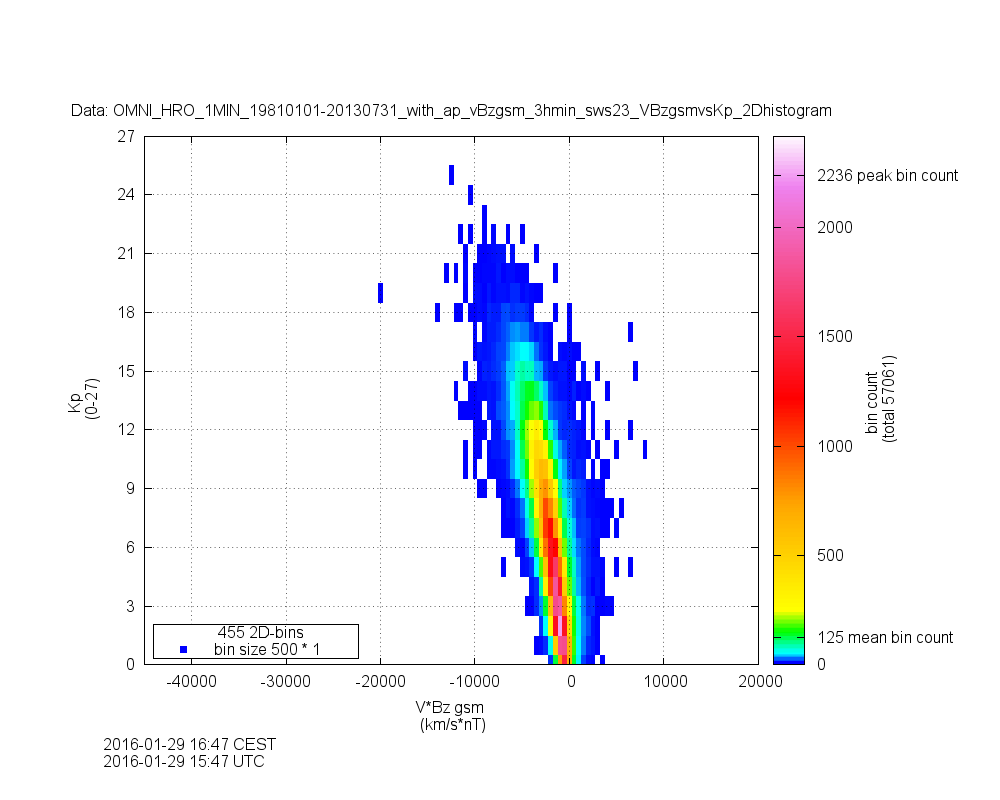
\includegraphics[width=0.3\textwidth]{images/gnuplots/OMNI_HRO_1MIN_19810101-20130731_with_ap_vBzgsm_3hmin_sws23_VBzgsmvsKp_2Dhistogram_plot.png}
	\caption{same as Figure~XX... with the non-CME data flagged by the solar wind structure list. sws23 VBzgsmvsKp}
	\label{fig:OMNI_HRO_1MIN_19810101-20130731_with_ap_vBzgsm_3hmin_sws23_VBzgsmvsKp_2Dhistogram_plot}
\end{figure}

sws1 VBzgsmvsKp see \autoref{fig:OMNI_HRO_1MIN_19810101-20130731_with_ap_vBzgsm_3hmin_sws1_VBzgsmvsKp_2Dhistogram_plot}
\begin{figure}[htb]
	\centering
	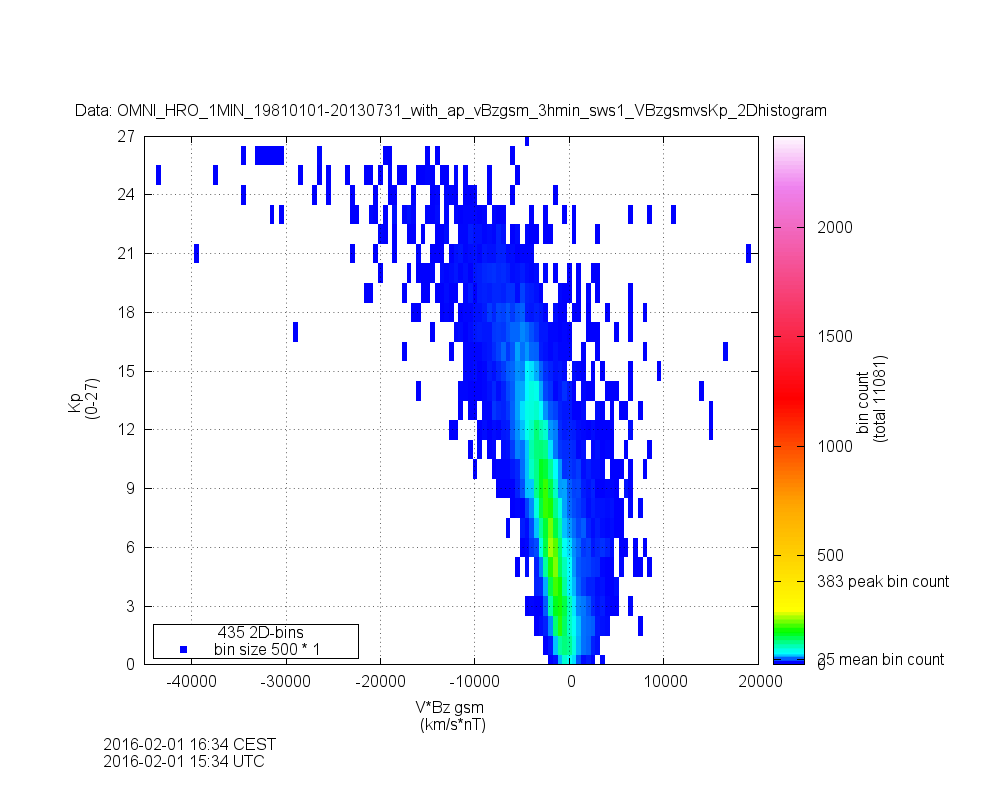
\includegraphics[width=0.3\textwidth]{images/gnuplots/OMNI_HRO_1MIN_19810101-20130731_with_ap_vBzgsm_3hmin_sws1_VBzgsmvsKp_2Dhistogram_plot.png}
	\caption{same as Figure~XX... with the CME data flagged by the solar wind structure list. sws1 VBzgsmvsKp}
	\label{fig:OMNI_HRO_1MIN_19810101-20130731_with_ap_vBzgsm_3hmin_sws1_VBzgsmvsKp_2Dhistogram_plot}
\end{figure}

CME- and non-CME 'comparison' see \autoref{fig:OMNI_HRO_1MIN_19810101-20130731_with_ap_vBzgsm_3hmin_sws_VBzgsmvsKp_comparison_plot}
\begin{figure}[htb]
	\centering
	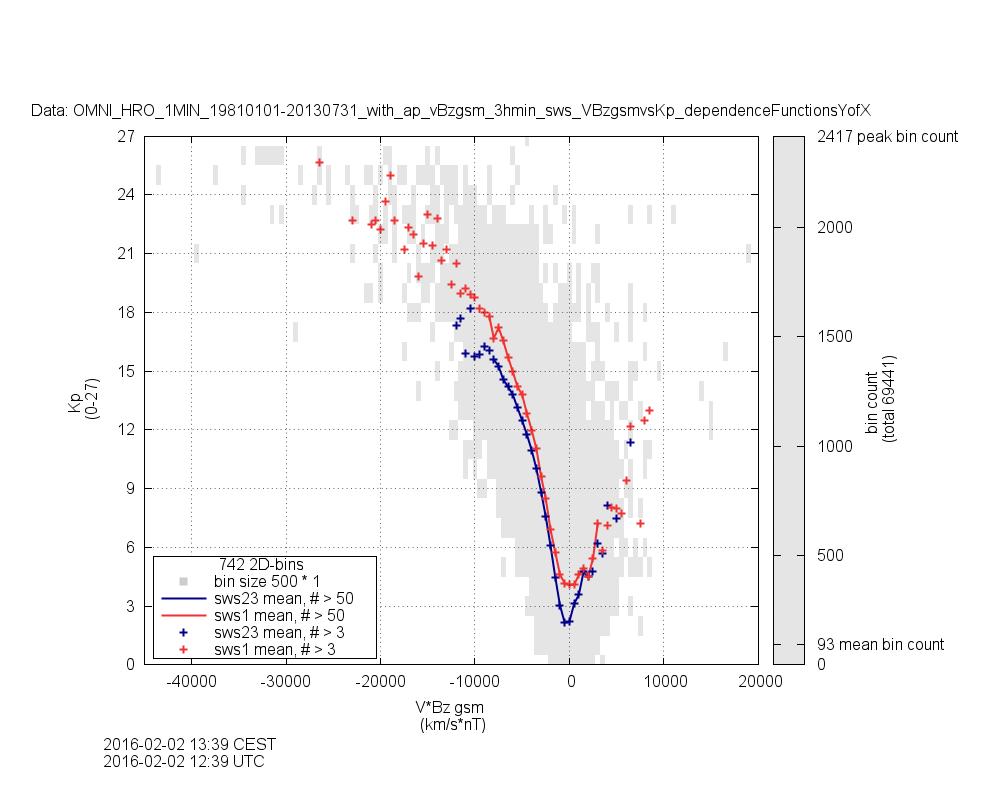
\includegraphics[width=0.3\textwidth]{images/gnuplots/OMNI_HRO_1MIN_19810101-20130731_with_ap_vBzgsm_3hmin_sws_VBzgsmvsKp_comparison_plot.png}
	\caption{Kp dependence on CME- and non-CME structures.}
	\label{fig:OMNI_HRO_1MIN_19810101-20130731_with_ap_vBzgsm_3hmin_sws_VBzgsmvsKp_comparison_plot}
\end{figure}



Kp vs VBzgsm - CMEs as fraction of overall solar wind; see \autoref{fig:OMNI_HRO_1MIN_19810101-20130731_with_ap_vBzgsm_3hmin_CMEpart_VBzgsmvsKp_2Dhistogram_plot}
\begin{figure}[htb]
	\centering
	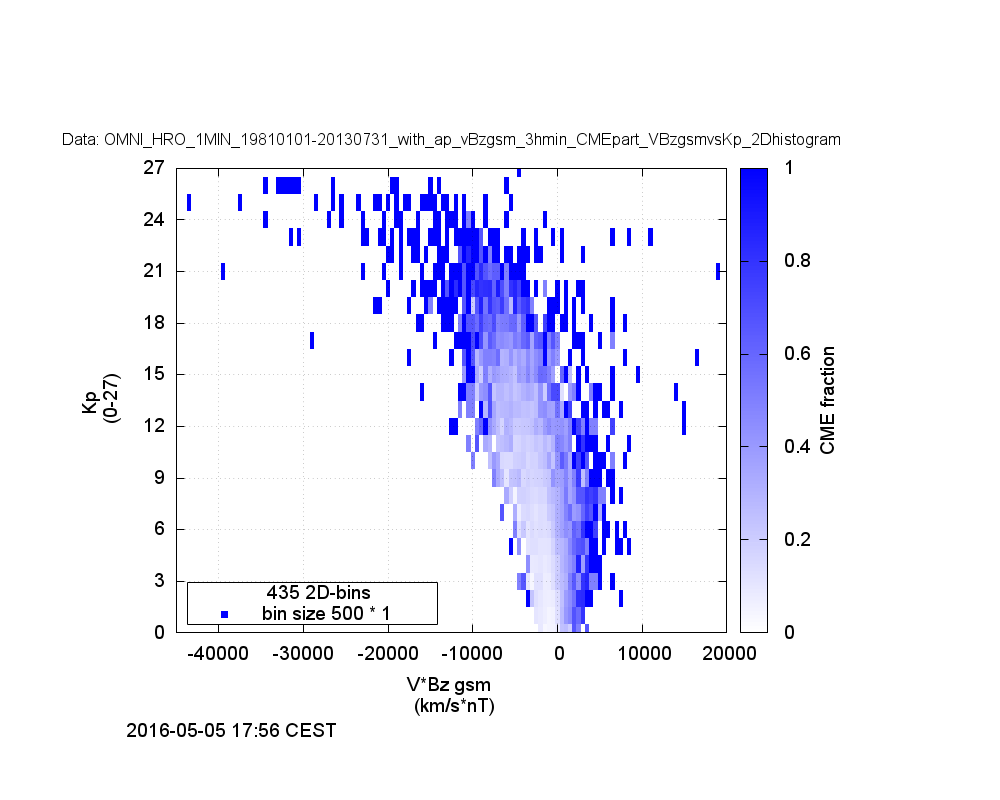
\includegraphics[width=0.3\textwidth]{images/gnuplots/OMNI_HRO_1MIN_19810101-20130731_with_ap_vBzgsm_3hmin_CMEpart_VBzgsmvsKp_2Dhistogram_plot.png}
	\caption{CMEs as fraction of overall solar wind. sws1/sws}
	\label{fig:OMNI_HRO_1MIN_19810101-20130731_with_ap_vBzgsm_3hmin_CMEpart_VBzgsmvsKp_2Dhistogram_plot}
\end{figure}


\section{Solar wind structure analyses}
%\label{sec:}

ACE solar wind time series (at 1\,au) and event list\\

see OPTIMAP events\\
?to analyse: ACE event lists\\
%method: automatic list creation by event detection via parameter thresholds

sample CME analyses (MVA, -> Kp)\\


\section{CME impact on the magnetosphere}

analyze sw coupling to the magnetosphere for being able to estimate CME impact from white light images (see paper draft...)\\

events from ACE CME list...\\

add OMNI ap->Kp values and sws flags\\
filter to sws1 and sws23 data\\
compare CME vs non-CME distributions (VBzgsmvsKp, VvsKp, BvsKp, BzgsmvsKp..)\\
get dependence functions\\


\section{Solar wind frequency distributions}

How often occur certain conditions?\\

OMNI hourly data\\
$v, B, T, n$\\
see \autoref{fig:histogram_V_plot}
%do all four figures...
\begin{figure}[htb]
	\centering
	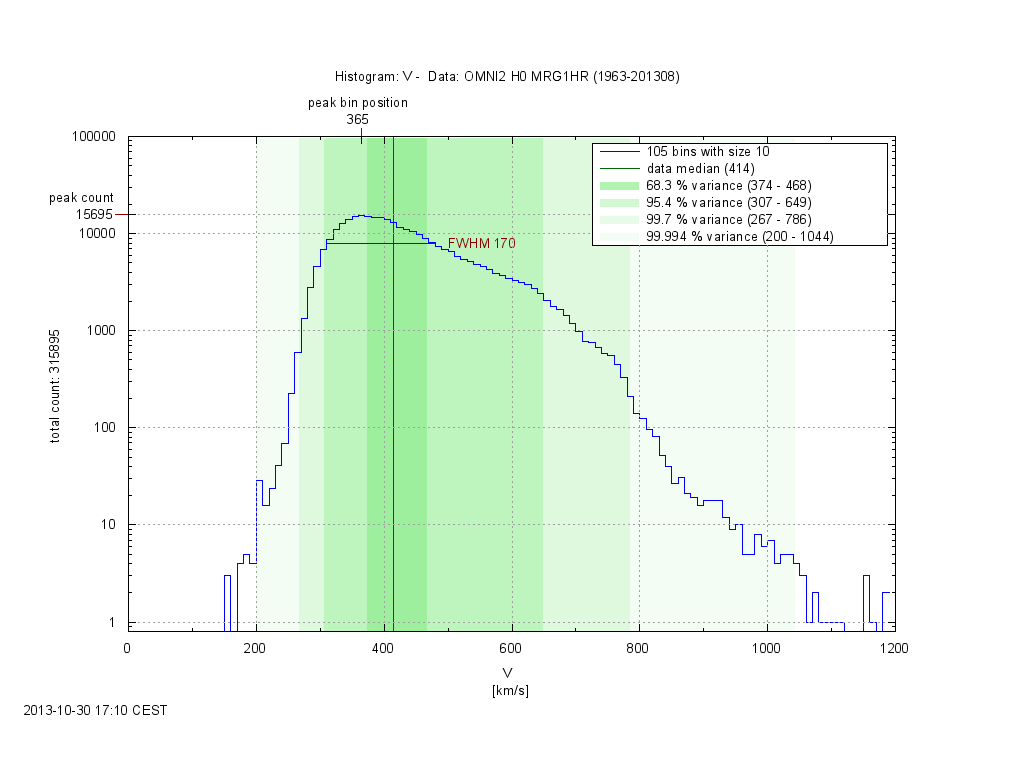
\includegraphics[width=0.3\textwidth]{images/gnuplots/histogram_V_plot.png}
	\caption{Histogram of solar wind velocity.}
	\label{fig:histogram_V_plot}
\end{figure}

%maybe couple with solar wind model...?\\

- overall frequency\\
- variation over the years (solar cycle)\\
- seasonal variation\\
- internal variation (HSS, LSS, CMEs)\\


\subsection{Solar wind solar cycle dependence}

%definition of 4 solar cycle phases?\\
%cycle dates: min, rise, max, set (maybe omit this?)\\

the density shows no obvious solar cycle dependence (look into it...)\\
the parameters V, T and B show a clear solar cycle dependence\\
see \autoref{fig:OMNI_yearly_freq_NVTBSSN_gps}
\begin{figure}[htb]
	\centering
	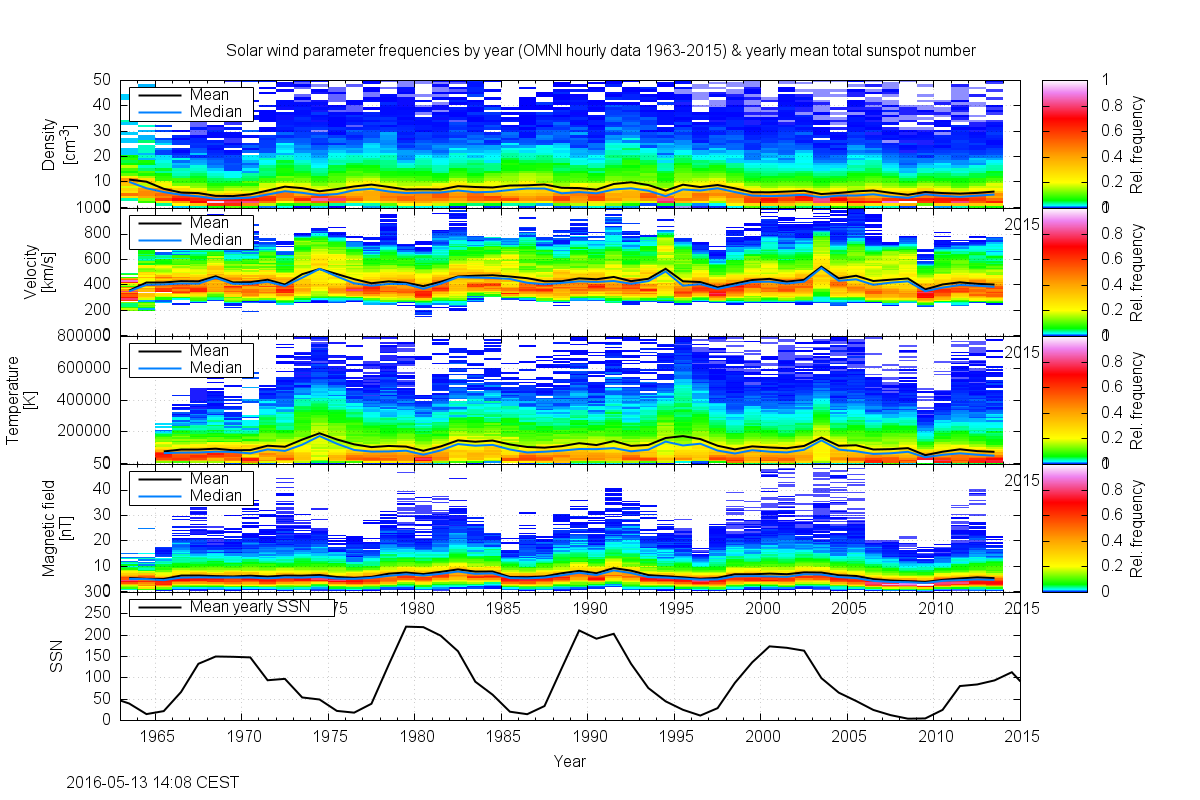
\includegraphics[width=0.3\textwidth]{images/gnuplots/OMNI_yearly_freq_NVTBSSN_gps.png}
	\caption{Plot of solar wind parameter frequencies and mean total sunspot number by year for the period 1963--2013. Density, velocity, temperature and magnetic field frequencies show more or less a solar cycle dependence, illustrated by the mean total sunspot number. SSN data from WDC-SILSO, Royal Observatory of Belgium, Brussels.}
	\label{fig:OMNI_yearly_freq_NVTBSSN_gps}
\end{figure}
add SSN matrix plot...\\


\subsection{Solar wind seasonal dependence}

seasonal variation\\
sw by month\\
quantify variation amplitudes\\

see \autoref{fig:OMNI_monthly_freq_V_gps}
%do all four figures...
\begin{figure}[htb]
	\centering
	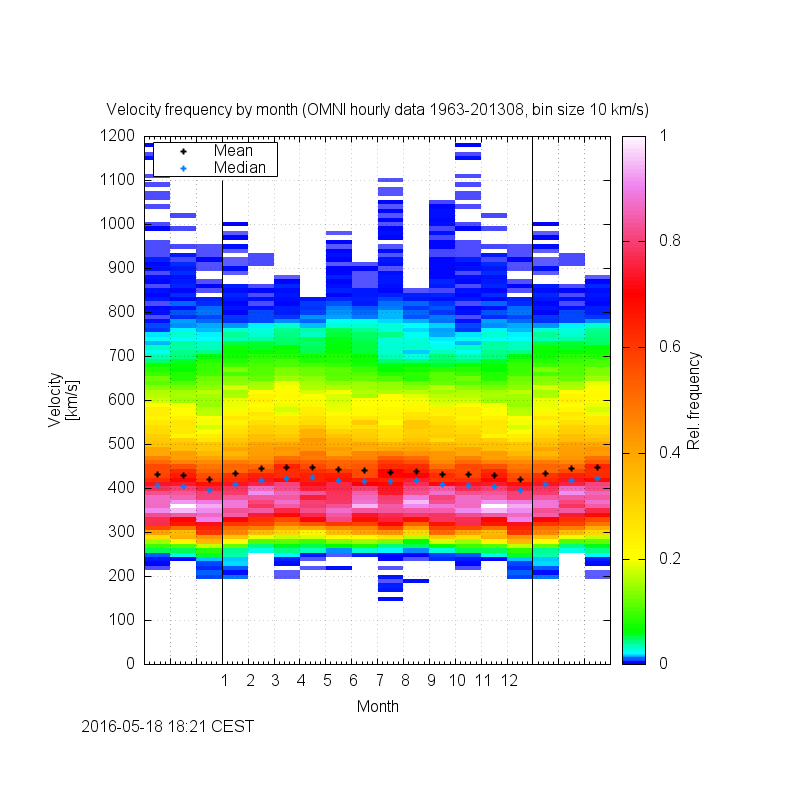
\includegraphics[width=0.3\textwidth]{images/gnuplots/OMNI_monthly_freq_V_gps.png}
	\caption{Diagram of the velocity frequency by month for the period 1963/01--2013/08. Mean and median values are shown as well.}
	\label{fig:OMNI_monthly_freq_V_gps}
\end{figure}


derived exponent values from simple trigonometric fit on monthly values:\\
$c_N = -2.234$\\
maybe figure?\\

...following maybe into section 'radial dependence of median value?\\
expected influence from perihelion/aphelion (see Appendix...) distance vs observations\\
we expect for the proton density (scaling law $N(r) = 7.6~\text{cm}^{-3} \cdot r^{-2}$):\\
N(0.983~au) = 7.9~cm$^{-3}$\\
N(1~au) = 7.6~cm$^{-3}$\\
N(1.017~au) = 7.3~cm$^{-3}$\\
we expect for the magnetic field strength (scaling law $\propto r^{-1.6}$):\\
B(0.983~au) = 6.3~nT\\
B(1~au) = 6.1~nT\\
B(1.017~au) = 5.9~nT\\


see \autoref{fig:OMNI_monthly_freq_B_a_gps}
%do all four figures...
\begin{figure}[htb]
	\centering
	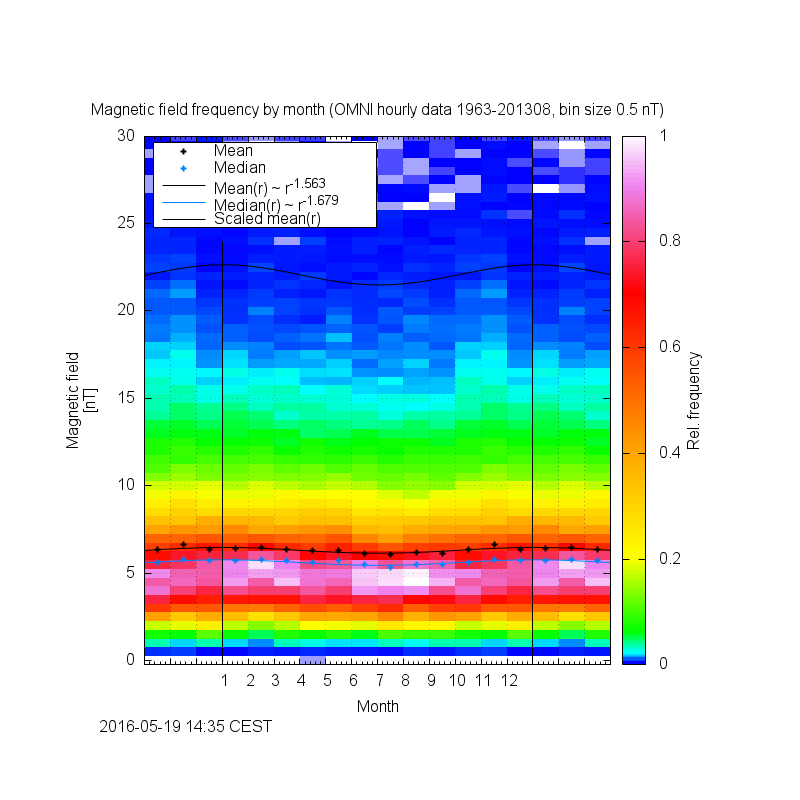
\includegraphics[width=0.3\textwidth]{images/gnuplots/OMNI_monthly_freq_B_a_gps.png}
	\caption{Diagram of magnetic field frequency by month for the period 1963/01--2013/08. Mean and median values are shown as well as the expected course from the solar distance variation (obtained from Helios data).}
	\label{fig:OMNI_monthly_freq_B_a_gps}
\end{figure}


\section{Kp frequency distribution}

Plot of the Kp frequency distribution (see \autoref{fig:histogram_Kp_plot})	%make better than VBTp129!
\begin{figure}[htb]
	\centering
	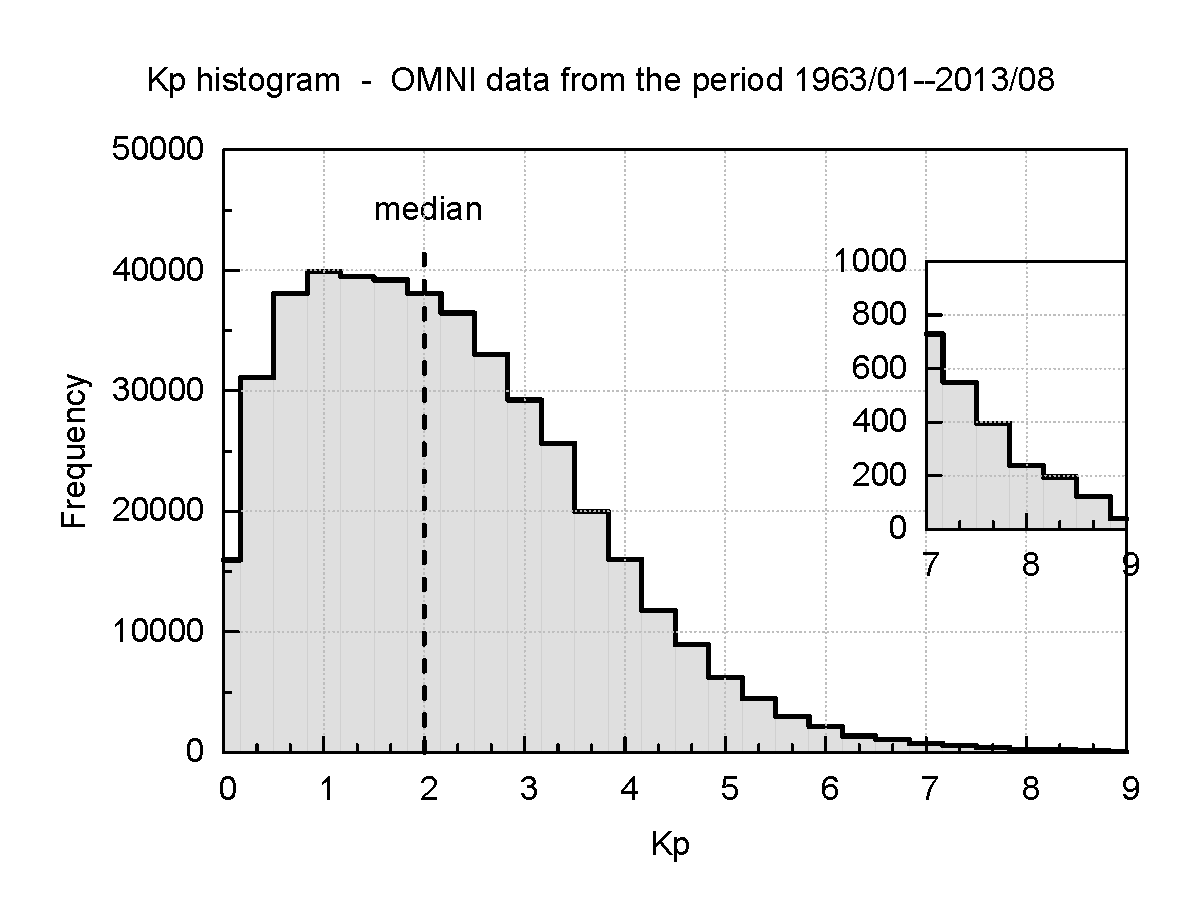
\includegraphics[width=0.3\textwidth]{images/gnuplots/histogram_Kp_plot.pdf}
	\caption{Kp frequency distribution for the period 1963/01--2013/08. The median Kp value is 2 and a Kp of 9o occurred only 39 times. OMNI data.}
	\label{fig:histogram_Kp_plot}
\end{figure}


\subsection{Kp solar cycle dependence}
%\label{sec:}

%cycle dates: min, rise, max, set (maybe omit this?)\\

- solar cycle variations\\
- variations between solar cycles\\

the yearly Kp frequency shows variations; the yearly mean Kp shifts about 2~units.\\
plot of the yearly Kp frequency (see \autoref{fig:Kp_freq_yearly_ssn_plot})
\begin{figure}[htb]
	\centering
	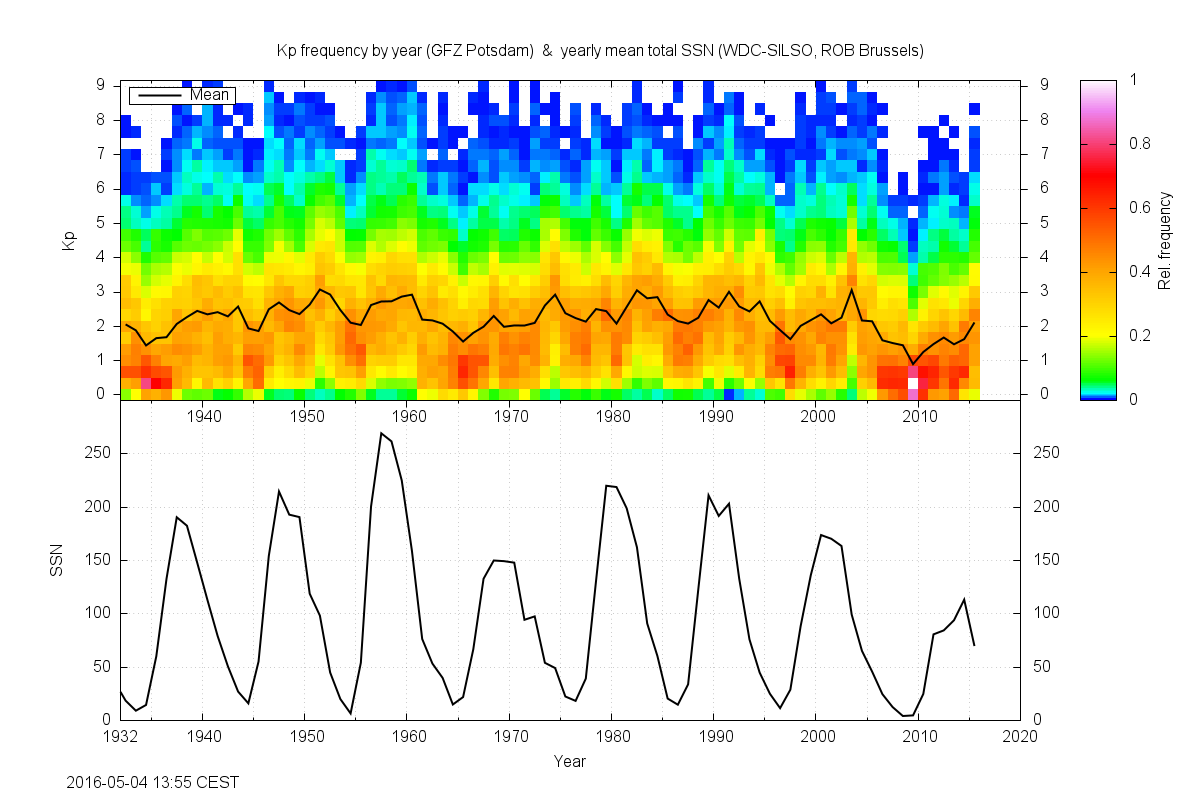
\includegraphics[width=0.3\textwidth]{images/gnuplots/Kp_freq_yearly_ssn_plot.png}
	\caption{Kp frequency by year, yearly mean Kp and yearly mean total SSN for the years 1932--2015. The pattern of Kp shows an imprint of the solar cycle. Kp data from GFZ German Research Centre for Geosciences, Potsdam, Germany and SSN data from WDC-SILSO, Royal Observatory of Belgium, Brussels.}
	\label{fig:Kp_freq_yearly_ssn_plot}
\end{figure}
add Kp--SSN matrix plot...\\

analyze Kp frequency by month for different SWSs\\
analyze Kp frequency by year for different SWSs\\
put into later part of analysis...


\subsection{Kp seasonal dependence}
%\label{sec:}

for high Kp values (>~4?) there are yearly frequency maxima at the equinoxes and minima at the solstices. this variation amounts to more than 1~Kp (see \autoref{fig:Kp_freq_monthly_plot})
\begin{figure}[htb]
	\centering
	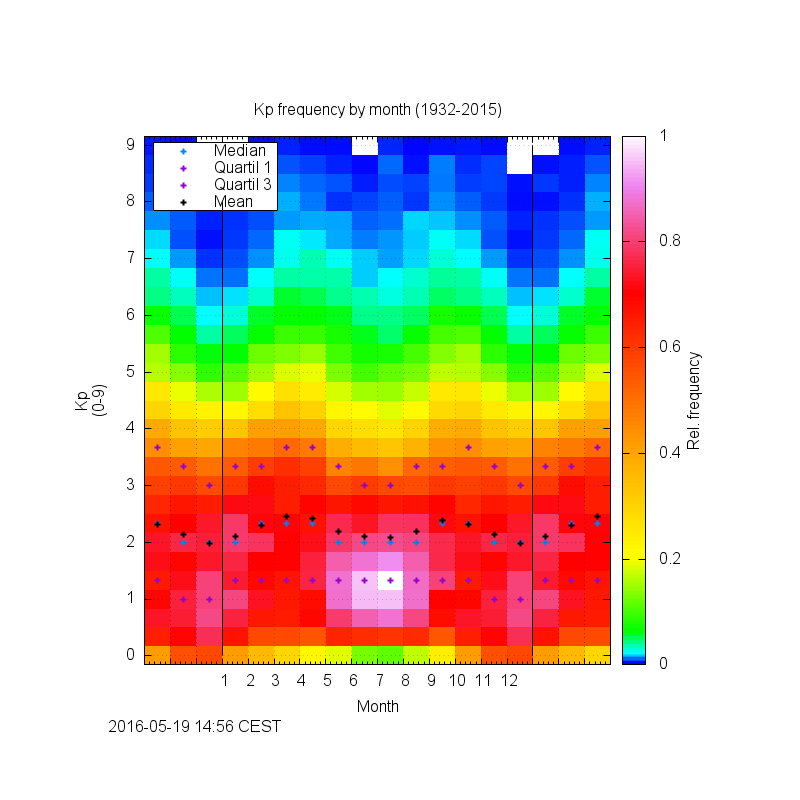
\includegraphics[width=0.3\textwidth]{images/gnuplots/Kp_freq_monthly_plot.png}
	\caption{Diagram of Kp frequency by month for the period 1932--2015. Median and quartil values are shown as well. remove mean...}
	\label{fig:Kp_freq_monthly_plot}
\end{figure}

possible causes (see \citet{Rangarajan1997} p. 1282 and mention Bartels1963 too
):\\
- Earth's rotation axis tilt ($\pm23.44$\textdegree) (obliquity to orbit/inclination of equator)\\
- solar rotation axis tilt ($\pm7.25$\textdegree) (cite 'NASA Earth fact sheet')\\
- varying distance from Sun 0.983--1.0167~au ($\pm3.3~\%$)\\
- changing solar cycle polarity gives two superimposed maxima... -> No. see even/odd plots\\

read Bothmer1998 Ch 3...\\


\section{Summary/Results}

sw-nowcast: vBzgsm-Kp relation (average and worst case)\\
CME-forecast: v-Kp relation (average and worst case)\\

seasonal correction: $\Delta$Kp(month)\\
$Kp_\text{impact} = Kp_\text{CME} \pm \Delta Kp(month)$\\

sw-timeseries ACE OPTIMAP ``Zeitreihe''-events

\section{Forecast}
%\label{sec:}

\subsection{Internal solar wind correlations}

B-V correlation\\
ACE MAGSWE 64~s data -> yearly overlay plot\\


\subsection{Kp forecast from CME velocity}

V-Kp correlation\\
similar to \citet{Elliott2013}; different data resolution and averaging method (3-hour maximum of 1~min data)

\section{Applications}

rssfeeds, rtsw plots\\
CME Kp impact\\
part of DDC\\


%%%%%%%%%%%%%%%%%%%- Solar wind evolution -%%%%%%%%%%%%%%%%%%%%%%%%

\chapter{Solar wind origin and evolution}
%\chapter{}

%COFI -- chapter outline and flow integration\\

talk about origin and evolution...\\

what is the aim?\\
- empirical analytical sw distribution model with radial dependence\\
- sw extrapolation to near-Sun region with an empirical sw model\\

Motivation?\\
- solar wind acceleration\\
- coronal heating problem\\
- SPP mission\\

new analyses of the Helios solar wind data\\

input (Helios data):\\
	magnetic field strength; proton velocity, number density and temperature\\

output (results):\\
	empirical distribution model for 0.29--0.98~au\\
	empirical distribution extrapolation model to near-Sun region\\
	L-> refined models with the combination of OMNI data\\
	
theory/literature:\\
existing model: \citep{Sittler1999}\\
L-> compare with their radial density function eq. (18a)\\
existing solar wind and CME measurements, steady state mass flow (eq.~(5)), velocity model v(r) \citep{Sheeley1997}\\
Helios results, radial gradients see Schwenn1990 p.~155\\
Schwenn1983 intro -> sw-averaging comment (beer and wine)\\)

\citet{Balogh1999} (origin and formation of CIRs in inner heliosphere with Helios data)\\

%see astro70/CGAUSS/dropbox_presis/...\\

see Hellinger2013 p.1353\\
see Balogh1999 from p. 162\\
and what differentiates our model from the others...\\\

model constraints:\\
see Marsch1999...\\

%see presi 1.07 Inside Helios-Origins and Evolution-Salem.ppt


\section{Solar wind parameters}	%for the region below 1~au

%Methods:
% 2016-08-28
% 	determine fit function type for radial dependency of Helios data
%		-> exponential regression fit
%		=> data mean(r) and median(r)
%	determine fit function type for frequency distribution of 1~au OMNI data
%		-> lognormal fit
%		-> double lognormal fit
%		=> weight parameter c
%	build exponential radial double lognormal function
%		-> fit that function to the radial frequency binned data
%		=> fit parameters define Helios sw model for [0.3--1~au]
%	evaluation of function behavior in direction of Sun up to 0.04~au
%		-> extrapolation not feasible with variable width -> constant width (constant sigma/shape)
%		-> single lognormal function sufficient; see WSSR
%	single lognormal fit with constant width
%		-> extrapolation model
%
%	Model variants:
%	- Helios replication model [0.3--1~au]
%	- Helios extrapolation model [0.04--1~au]
%	OMNI 1~au median (mean?) value of specified period:
%	- all-time extrapolation model (mean model with whole OMNI period)
%	- current extrapolation model (current year median or so)
%	- forecast extrapolation model (that years solar cycle historic median)
%
%	boundary conditions:
%	- 1~au OMNI data
%	- continuity of mass flux


motivation/reason for necessity?/why?\\

which parameters? (major solar wind parameters)\\
- The characteristic behavior of a plasma is determined by its density, temperature and magnetic field strength. cite?\\
- the velocity is the defining parameter of the solar wind\\

definition of 'the four solar wind parameters':\\	%by OMNI histograms
	magnetic field strength, aka magnetic field, $B$, usually measured in nT, in the order of 0--35~nT at 1~au\\
	proton bulk velocity, aka velocity, $v$, usually measured in km/s, in the order of 200--900~km/s at 1~au\\
	proton number density, aka density, $n$, usually measured in cm$^{-3}$, in the order of 1--60 at 1~au\\
	proton temperature, aka temperature, $T$, usually measured in K, in the order of 10\,000--1\,000\,000~K at 1~au\\
sentence about ordering of the parameters...\\


%data binning
hourly OMNI data\\
measurement precision:\\
$B$: 0.01~nT\\
$v$: 1~km/s\\
$n$: 0.1~cm$^{-3}$\\
$T$: 1~K ? (smallest found: 7~K)\\

error discussion:\\
OMNI hourly data mean:\\
$B$: bin size 0.5~nT, median 5.6, mean 6.30056(18)\\
$v$: bin size 10~km/s, median 414, mean 437.6700(18)\\
$n$: bin size 1~cm$^{-3}$, median 5.3, mean 6.831410(18)\\
$T$: bin size 10\,000~K, median 80\,751, mean 112\,219.0(19) (with 1000~K as precision)\\

empirical data; Helios; hourly\\
why hourly and not higher resolution data?\\
measurement precision:\\
$B$: 0.01~nT\\
$v$: 0.1~km/s\\
$n$: 0.1~cm$^{-3}$\\
$T$: 100--1000~K (3 digits)\\
$r$: 0.01~au\\

error discussion:\\
Helios hourly data mean:\\
$B$: min 337, precision: 0.000545; 18.3x better\\
$v$: min 497, precision: 0.00449; 22.2x\\
$n$: min 497, precision:  0.00449; 22.2x\\
$T$: min 497, precision: 4.49--44.49 22.2x\\
=> so we use 1/10 the measurement precicion for the mean.\\

median precision same as data precision\\


\section{Empirical solar wind model}

Helios data ranges:\\
- time range [1974-12-10--1980-03-04]\\
- solar distance range 0.29--0.98~au\\
- 0°--360° longitude\\
- latitude range -7.25°--7.25°\\
data constrictions:\\
- hourly data\\
- data gaps -> uneven coverage -> solar cycle minimum dominates\\
- limited parameter ranges\\

model boundaries (spherical coordinates):\\
- mean solar wind of the Helios time range\\
- solar distance range 0.29--0.98~au\\
- rotational symmetry\\
- confined to ecliptic\\
model constrictions:\\
- radial dependency function\\
- frequency distribution function\\

all assumptions outside these boundaries are extrapolations with large uncertainties...\\

%latitude variation negligible?
influence from latitude variation in data negligible? (see Ulysses figure in introduction). Helios probes within ecliptic => variation span equal to solar tilt: -7.25° to 7.25°; solar tilt/obliquity to ecliptic: $i_\odot = 7.25\degree$ (Sun fact sheet: \url{http://nssdc.gsfc.nasa.gov/planetary/factsheet/sunfact.html)}\\
big part of Helios data is from latitudes $>\pm5$°, see Figure~XX (data count over latitude) and see Figure~XX (Helios orbit polar plane in data section...)\\
As we see at the end of this chapter in Section~XX, the latitude influence is negligible and so we assume it to be constant for our models.\\
see also \citet{Richardson1995}\\
see also \citet{Schwenn1990} p.~127\\

%%%%%%%%%%%%%%%%%%%%%%%%%%
approach:
\begin{itemize*}
	\item determine fit function type for radial dependency of Helios data
	\item determine fit function type for frequency distribution of OMNI data
	\item fit exponential radial double lognormal function to binned Helios data
	\item evaluation of function behavior in direction of Sun up to 0.04~au
	\item single lognormal fit with constant width is extrapolation model
	\item model evaluation
	\item some model variants with OMNI median values
\end{itemize*}


\subsection{Solar distance dependency---theory}
%\label{sec:}

%why both median and mean?\\

heliospheric distance $r$\\
averages: median(r), mean(r)\\

solar wind parameter distributions and their radial dependence from theory/literature:\\
B-field radial profile: $B \propto r^{-.5?}$\\
	Kivelson/Parker references\\
	shear effect from solar rotation; talk 2014-07-21\\
velocity radial profile: $V \propto r^{0?}$\\
	model based on LeBlanc1998 electron density with flux conservation: Zic2015(Temmer)\\
	Parker...\\
density radial profile: $N \propto r^{-2}$\\
	simple view: for a spherical constant velocity mass outflow a one over distance squared law is expected because of the mass flux conservation per solid angle for different distances. measurements up to the outer heliosphere confirm the $1/r^2$ dependency (1--38~au by Voyager~2, \citep{Belcher1993} newer paper?)\\
	electron density model corona--1~au LeBlanc1998\\
	radial electron density from Helios $6.14r^-2.10$ compared to radio bursts see Bougeret1983\\% (not Bothmer1998 and not Schwenn1990 book)\\
	existing electron density model see Leblanc1998\\

	in an ideal neutral plasma the electron and proton number density have the same values (neutral plasma) (reference?)\\
	ca. 10~\% more electrons than protons (due to alphas) cite?\\	%http://omniweb.gsfc.nasa.gov/ftpbrowser/bow_derivation.html\\
	radial electron density models suggest a proportionality to $r^{-2}$ for $r > 10~R_\odot$ (leblanc1998 with its Figure~6)\\
temperature radial profile: $T \propto r^{-1?}$\\
	at larger distances heating outbalances the adiabatic temperature part (adiabatic cooling vs. pickup proton and stream--interaction heating; 1--68~au by Voyager~2; \citet{Richardson2003}\\


solar wind ram pressure $p_\text{ram} = \rho V^2$\\

conserved quantities:\\
- momentum conservation... VBbookp112\\
- flux conservation...\\

%%%%%%%%%%%--  flux  --%%%%%%%%%%%%%%%
%As Schwenn1983 stated ``From Helios in situ measurements we know that at least beyond 0.29~au there is almost no nonradial flow, on the average. In fact, the particle flux was found to be that quantity which varies the least with increasing R.''\\

%Schwenn1990:
%increase in sw velocity with distance; speed increase mainly in slow solar wind
%density deviates from a purely r^-2 fall-off (10% faster); n(r)=6.1*r^-2.1 cm^-3; different behavior in slow and fast wind
%proton flux density constant between 0.3-1.0~au -> no meridional flow into/out of the ecliptic; different for slow and fast sw

With consideration of continuity the mass flux per solid angle has to be constant: $\dot{m} = \text{const}$\\
conserved quantities:\\
- mass flux: $\dot{m} = \rho v A$ (with mass density $\rho$, velocity $v$ and [cross-sectional area $A$] or solid angle?...)\\
- particle fluxes (proton flux, electron flux, etc.)\\
	- proton flux: $j_\text{p} = n_\text{p} v_\text{p} A$ (with proton density $n_\text{p}$ and proton velocity $v_\text{p}$)\\

(with proton mass density $\rho = n_\text{p} m_\text{p}$ (with proton number density $n_\text{p}$ and proton mass $m_\text{p}$).)\\

the individual radial dependencies for a spherical radial outflow are:\\
$A(r) \propto r^2$ --> $A/r^2 = \text{const}$\\
and assuming an exponential dependency,\\
$n_{\text{p}}(r) = n_0 r^{c_n}$,\\
$v(r) = v_0 r^{c_v}$\\
\begin{align}
	j_\text{p} &= \text{const}\\
	n_\text{p} v_\text{p} A &= \text{const}\\
	n_0 r^{c_n} v_0 r^{c_v} r^2 &= \text{const}\\
	r^{c_n} r^{c_v} r^2 &= \text{const}\\
	\Rightarrow c_n + c_v + 2 &= 0\\
	c_n + c_v &= -2
\end{align}
an increasing velocity should result in a steeper density...\\

validity of mass flux continuity: within the heliosphere mass to energy conversion and vice versa is negligible, but there can be flux from and to higher latitudes as the Helios data is localized to a small latitude range in the ecliptic plane.\\
estimate the error from that... (if error is too big => drop continuity condition)\\
larger errors should be located near CMEs and CIRs (nonradial flows from interactions)\\
there is a proton flux difference between slow and fast solar wind streams (see book Schwenn1990 p.~146)

estimate the possible size of error:\\
mean:\\
$c_n = -2.010$\\
$c_v = 0.049$\\
$c_n + c_v = -1.961$\\
difference to -2 is 0.039\\
% [median:\\
% $c_n = -2.093$\\
% $c_v = 0.058$\\
% $c_n + c_v = -2.035$\\
% difference to -2 is -0.035\\
% ]constant mass flux only for mean...\\


\subsection{Solar distance dependency---Helios data}

we want to obtain the solar distance dependence of the mean and the median of the Helios data\\

%data
we use hourly Helios data...\\
the hourly Helios data has a native radial resolution of 0.01~au, so for calculating the median the data is binned into 0.01~au bins\\

%why exponential function?
we expect an exponential behavior from all four parameters (see radial dependence theory section with literature references)\\
=> therefore we use an exponential regression fit function $f(r) = a\,r^b$.\\
fit weighting by counts per bin\\

%fit result figures
the resulting fit curves are displayed in \autoref{fig:radial_fit_4_thesis_pdfcairo_plot}. Larger individual Graphs can be found in the appandix (Figures~XX).%\ref{fig:radial_fit_Bv_thesis_pdfcairo_plot} and \ref{fig:radial_fit_nT_thesis_pdfcairo_plot}).
\begin{figure}[htb]
	\centering
	\includegraphics[width=1\textwidth]{images/gnuplots/radial_fit_4_thesis_pdfcairo_plot.pdf}
	\caption{Plots of the four solar wind parameters over solar distance. The mean and median per 0.1~au data bin and their fit curves (weighted with data count) are plotted as well.}
	\label{fig:radial_fit_4_thesis_pdfcairo_plot}
\end{figure}

flux figure...\\


%state this at the first occurence... (from GUM guide)
%“mS = 100,021 47(35) g, where the number in parentheses is the numerical value of (the combined standard uncertainty) uc referred to the corresponding last digits of the quoted result.”

%fit result table
With $r$ in astronomical units one gets the fit coefficient values of all four parameters as seen in \autoref{tab:mean_median_fit_parameter}.
\begin{table}[htb]\small
	\centering
	\captionsetup{belowskip=4pt}
	\caption{These are the fit coefficients for the median and mean solar distance dependence functions of the four plasma parameters from the combined Helios data set. The errors in brackets are the estimated standard deviation of each fit parameter. remove units?}
	\begin{tabular}{lrrcrrc}
		\toprule
		\multirow{2}{*}{Parameter}	&\multicolumn{2}{c}{Median}	&	&\multicolumn{2}{c}{Mean}	&mean=median\\
		\cmidrule{2-3}	\cmidrule{5-6}
			&\multicolumn{1}{c}{$a$}	&\multicolumn{1}{c}{$b$}	&	&\multicolumn{1}{c}{$a$}	&\multicolumn{1}{c}{$b$}	&$r_\text{equal}$\\
		\midrule
		Magnetic field	&5.377(92)~nT	&-1.655(17)	&	&6.05(10)~nT		&-1.546(18)	&0.344~au\\
		Velocity	&410.7(28)~km/s	&0.058(13)	&	&435.6(24)~km/s	&0.049(10)	&692~au\\
		Density		&5.61(27)~cm$^{-3}$	&-2.093(46)	&	&7.57(30)~cm$^{-3}$	&-2.010(38)	&0.027~au\\
		Temperature	&7.14(23)$ \times 10^4$~K	&-0.913(39)	&	&9.67(21)$ \times 10^4$~K	&-0.792(28)	&0.081~au\\
		Flux		&fit coeffients...\\
% 		Magnetic field strength	&6.04753	&-1.54631&		&5.37723	&-1.65464	&0.344132483292368\\
% 			&(0.104689)	&(0.0176562)	&	&(0.0919207)	&(0.0171401)\\
% 		Velocity	&435.645	&0.049139	&	&410.72	&0.0580215	&692.392\\
% 			&(2.44896)	&(0.0103927)	&	&(2.81328)	&(0.0127228)\\
% 		Proton density	&7.56767	&-2.00987	&	&5.61317	&-2.09257	&0.027048\\
% 			&(0.300872)	&(0.0384042)	&	&(0.269386)	&(0.0459336)\\
% 		Temperature	&96\,743.2	&-0.792253&		&71\,388.5	&-0.913317	&0.081232928\\
% 			&(2143.64)	&(0.0280191)	&	&(2290.7)	&(0.0389327)\\
		\bottomrule
	\end{tabular}
	\label{tab:mean_median_fit_parameter}
\end{table}
%\captionsetup{width=0.75\textwidth}
%align caption width with table width  OR  widen table to textwidth

skewing of distributions...\\
its change...\\
for the magnetic field strength the mean and median cross each other at 0.344~au.\\


\subsection{Latitude dependency---theory}

refer to Ulysses figure...\\
Ulysses swoops polar plots...\\
see Schwenn1990's~Fig.~3.14\\


\subsection{Latitude dependency---Helios data}

latitude; see \autoref{fig:latitude_frequency_4_thesis_plot}
\begin{figure}[htb]
	\centering
	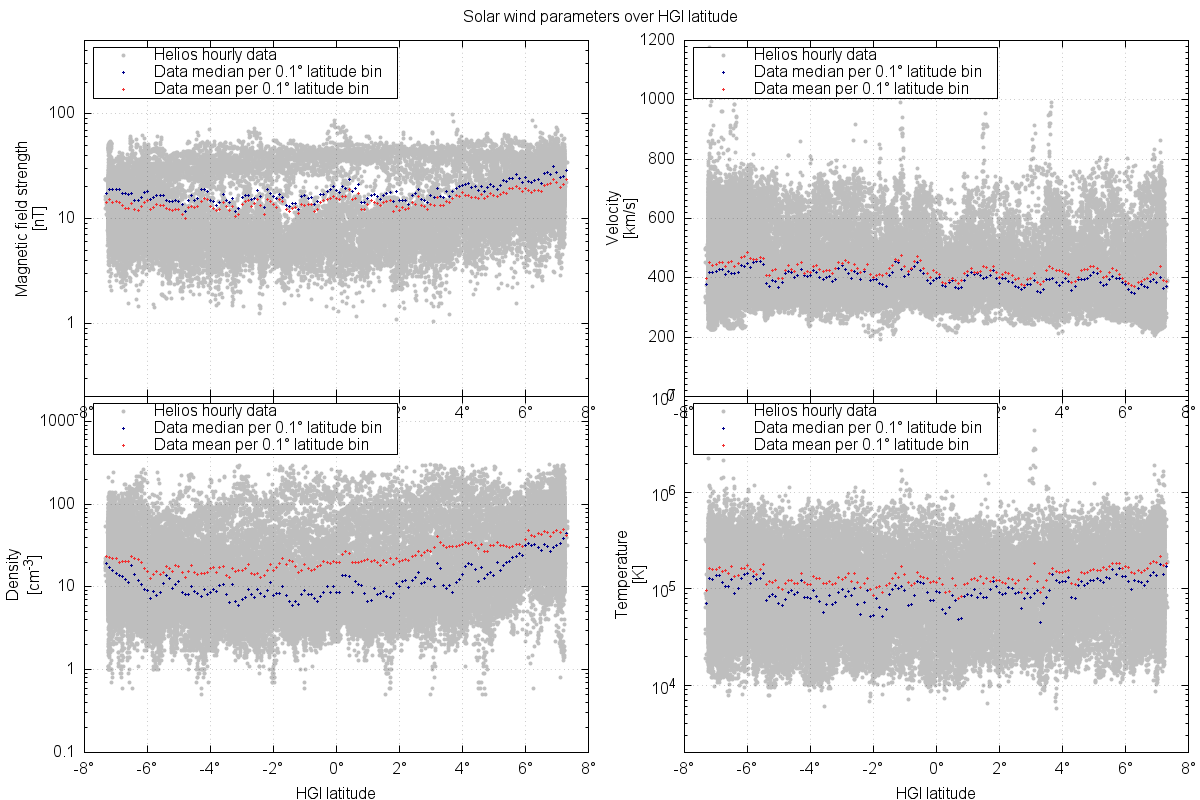
\includegraphics[width=0.5\textwidth]{images/gnuplots/latitude_frequency_4_thesis_plot.png}
	\caption{The four solar wind parameter's HGI latitude dependency. Their mean values per 0.1° bin are plotted as well. make figure same dimensions as projected figure in analysis part...}
	\label{fig:latitude_frequency_4_thesis_plot}
\end{figure}

with the exponential dependencies to 1~au projected solar wind parameters; there are only small changes with latitude in the range -7.25°--7.25°\\
have a look on distribution widths...\\

dependence from latitude in interval -7.25°--7.25° in Helios data negligible?, see \autoref{fig:latitude_frequency_rcorrected_v3_4_thesis_plot}.
\begin{figure}[htb]
	\centering
	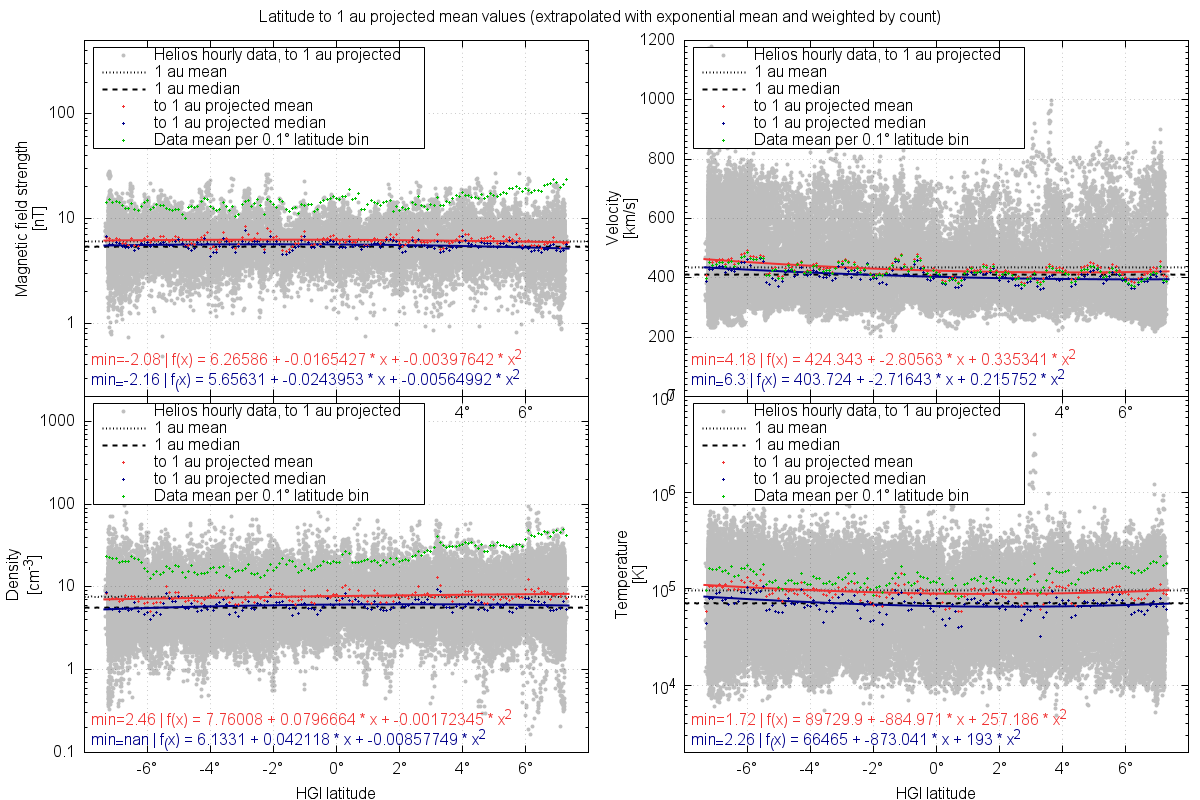
\includegraphics[width=0.5\textwidth]{images/gnuplots/latitude_frequency_rcorrected_v3_4_thesis_plot.png}
	\caption{Plot of the to 1~au projected solar wind parameters over latitude. And their mean values, including weighted fit. add projected median...}
	\label{fig:latitude_frequency_rcorrected_v3_4_thesis_plot}
\end{figure}
estimate error ranges...\\

plot Ulysses data into plot...\\


\subsection{Shape of the frequency distributions}
%\label{sec:}

%aim?
getting shape of the general distributions.\\

%how?
fitting the shape of the parameter's frequency distribution\\

%choice of distribution function?/why lognormal function?\\
Obviously the possible values for all four parameters are positive. This hints to the supposition that they are lognormally distributed, as many positive natural quantities conform to a lognormal distribution. This distribution is described by the lognormal function (For more on lognormal distributions see appendix \autoref{sec:lognormal_distribution}).\\
% * back up with literature references for solar wind parameters AND/OR figure

%fitting method
Therefore we use the lognormal function as a fit function in the process of the least squares regression fitting.\\
%data basis
To evaluate how well the lognormal function represents the solar wind distributions, the abundance of OMNI data (>50~years at 1~au) is more suited than the Helios data (few weeks summed at fixed solar distance), because it enables the averaging over long-time variations like the solar cycle.\\
As basis for the fit in situ solar wind data from the OMNI data set is used (see Section~XX... data section). More precisely, it is hourly data of the whole time range 1963/01--2013/08.\\

%data binning
Helios histogram bin size for mean of frequency distribution (at specific solar distance)\\
$B$: bin size 0.5~nT, min 337, mean precision: 0.000545\\
$v$: bin size 1~cm$^{-3}$, min 497, mean precision: 0.00449\\
$n$: bin size 10~km/s, min 497, mean precision:  0.00449\\
$T$: bin size 10\,000~K, min 497, mean precision: 4.49--44.49\\


\subsubsection{Single lognormal fit}
%single lognormal fit

%fit function
The lognormal fit function
\begin{align}
	W(x) &= \frac{1}{\sigma \sqrt{2 \pi} x} \, \text{e}^{- \frac{(\ln x - \mu)^2}{2 \sigma^2}}	\label{eq:single_lognormal_fit_function}
\end{align}
has two variables, the location ($\mu$) and the shape parameter ($\sigma$) (see also Appendix~XX). The distribution's mean and median postitions are easier to interprete and can directly be calculated from $\mu$ and $\sigma$ (see also Appendix~XX):\\
$median = \text{e}^\mu$\\
$mean = \text{e}^{\left(\mu + \frac{\sigma^2}{2}\right)}$\\
Their values, obtained from the fitting of the four solar wind frequency distributions, are listed in \autoref{tab:single_lognormal_fit_parameters}.
\begin{table}[htb]\small
	\centering
	\captionsetup{belowskip=4pt}
	\caption{These are the resulting fit coefficients $\mu$ and $\sigma$ from the fitting of the lognormal function (\ref{eq:single_lognormal_fit_function}) to the shape of the frequency distributions. The median and mean values and the standard deviation of the fit are shown as well. The values in brackets are the estimated standard deviation of each parameter.}
	\begin{tabular}{lrr.{3.11}.{3.11}.{1.2}}
		\toprule
		Parameter	&\multicolumn{1}{c}{$\mu$}	&\multicolumn{1}{c}{$\sigma$}	&\multicolumn{1}{c}{Median\up{a}}	&\multicolumn{1}{c}{Mean\up{a}}	&\multicolumn{1}{c}{stdfit [$10^{-3}$]}\\
		\midrule
		Magnetic field	&1.7361(28)	&0.4150(24)	&5.675(16)	&6.186(19)	&1.3\\
		Velocity	&6.0146(49)	&0.2182(40)	&409.4(20)	&419.2(21)	&2.9\\
		Density		&1.6660(47)	&0.6448(39)	&5.291(25)	&6.514(35)	&1.7\\
		Temperature	&11.2917(19)	&0.9086(16)	&8.015(15) \times 10^4	&1.2111(29) \times 10^5	&0.16\\
%data
% 		Magnetic field	&1.73613	&0.414970	&5.67534~nT	&6.18564~nT\\
% 		Velocity	&6.01461	&0.218165	&409.367~km/s	&419.225~km/s\\
% 		Density		&1.66602	&0.644791	&5.29109~cm$^{-3}$	&6.51366~cm$^{-3}$\\
% 		Temperature	&11.2917	&0.908564	&80\,152.9~K	&121\,108~K\\
%data error...
% 		Magnetic field	&0.00284807	&0.00235466	&0.016	&0.019\\
% 		Velocity	&0.0049	&0.0040	&2.0	&2.1\\
% 		Density		&0.0047	&0.0039	&0.025	&0.035\\
% 		Temperature	&0.0019	&0.0016	&152	&290
		\bottomrule
		\multicolumn{5}{l}{\footnotesize{\up{a}Values in their respective units nT, km/s, cm$^{-3}$ and K.}}
	\end{tabular}
	\label{tab:single_lognormal_fit_parameters}
\end{table}

describe figures; see \autoref{fig:histogram_fits_4_paper_pdfplot}
\begin{figure}[htb]
	\centering
	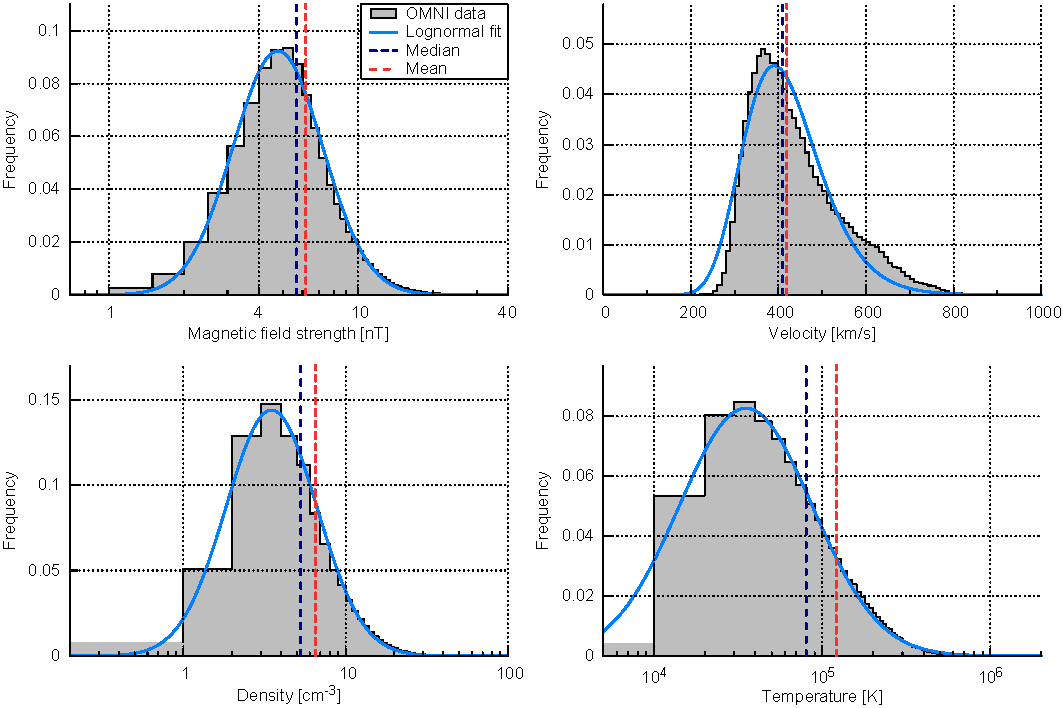
\includegraphics[width=1\textwidth]{images/gnuplots/histogram_fits_4_paper_pdfplot.pdf}
	\caption{The frequency distributions of the four solar wind parameters and their lognormal fits. The histograms have bins of 0.5~nT, 10~km/s, 1~cm$^{-3}$ and 10\,000~K and are based on the hourly OMNI data set. The fit's median and mean values are indicated as well.}
	\label{fig:histogram_fits_4_paper_pdfplot}
\end{figure}

%fit quality
From visual inspection, the resulting curves match well with the shape of the magnetic field strength, density and temperature distributions (\autoref{fig:histogram_fits_4_paper_pdfplot}). But for the velocity the fit function seems insufficient in describing its more complex shape.\\
From the normed stdfit values (\autoref{tab:single_lognormal_fit_parameters}) the velocity...\\

discuss high-value tail figures...\\

%gnuplot:
%sum of the squared differences or 'residuals' (SSR) between the input data points and the function values, evaluated at the same places. This quantity is often called 'chisquare' 
%'stdfit', the standard deviation of the fit, which is the rms of the residuals, and the variance of the residuals, also called 'reduced chisquare' when the data points are weighted.
%The 'sum of squares of residuals', also called 'chisquare', is the WSSR between the data and your fitted function; fit has minimized that.
%The WSSR can be used to calculate the reduced chisquare (WSSR/ndf) or stdfit, the standard deviation of the fit, sqrt(WSSR/ndf). Both of these are reported for the final WSSR.



%justification for compositional lognormal fit
To reach better fit results for the velocity the fit function has to be changed. We do not want to abandon the well-founded application of lognormal functions. But it is reasonable to assume that the distributions are composed of multiple branches (why?; slow/fast solar wind; literature; introduction). Therefore a compositional approach promises better fit results, which is why in the following we combine two lognormal functions.\\


\subsubsection{Double lognormal fit}

why only two? -> to keep it simple; every additional function adds further fit variables\\
compositional (two functions) lognormal regression fit\\

For the compositional regression fitting we use a function $W_\text{II}(x)$ which is composed of two lognormal distributions $W_1(x)$ and $W_2(x)$. The balancing parameter $c$ ensures that the resulting function remains normalized.
\begin{align}
	W_\text{II}(x) &= c \cdot W_1(x) + (1 -c) \cdot W_2(x)\\
	&= \frac{c}{\sigma_1 \sqrt{2 \pi} x} \, \text{e}^{- \frac{(\ln x - \mu_1)^2}{2 {\sigma_1}^2}} + \frac{(1 - c)}{\sigma_2 \sqrt{2 \pi} x} \, \text{e}^{- \frac{(\ln x - \mu_2)^2}{2 {\sigma_2}^2}} \label{eq:double_lognormal_fit_function}
\end{align}

The fitting of $W_\text{II}(x)$ to the frequency distributions gives the values of the five fit para\-meters ($c, \sigma_1, \mu_1, \sigma_2, \mu_2$), which are listed in \autoref{tab:double_lognormal_fit_parameters}.\\

The median of the composed distribution can be derived via solving
\begin{align}
	\int W_\text{II}(x)\,\text{d}x &= 0\\
	\intertext{and the mean via solving}
	\int x\,W_\text{II}(x)\,\text{d}x &= 0	\,.
\end{align}
Their values are listed in \autoref{tab:double_lognormal_fit_parameters}.
\begin{table}[htb]\small
	\centering
	\captionsetup{belowskip=4pt}
	\caption{These are the resulting fit coefficients from the double lognormal function (\ref{eq:double_lognormal_fit_function}) for the four examined solar wind parameters. The derived median and mean values are listed as well. Precision? Fit error in brackets.}
	\begin{tabular}{lcc.{2.8}.{1.8}ccccc}
		\toprule
		Parameter	&fkt	&\multicolumn{1}{c}{$c$}	&\multicolumn{1}{c}{$\mu$}	&\multicolumn{1}{c}{$\sigma$}	&\multicolumn{1}{c}{Median\up{a}}	&\multicolumn{1}{c}{Mean\up{a}}	&stdfit [$10^{-4}$]\\
		\midrule
		\multirow{2}{*}{Magnetic field}	&f1	&0.8656(79)	&1.7450(13)	&0.4631(23)	&\multirow{2}{*}{5.6570(X)}	&\multirow{2}{*}{6.769(X)}	&\multirow{2}{*}{3.1}\\
			&f2	&-	&1.6981(26)	&0.2061(50)	&	&	&\\
		\cmidrule{2-5}
		\multirow{2}{*}{Velocity}	&f1	&0.502(59)	&5.911(27)	&0.138(14)	&\multirow{2}{*}{413.4(X)}	&\multirow{2}{*}{439.1(X)}	&\multirow{2}{*}{6.6}\\
			&f2	&-	&6.1997(52)	&0.2117(40)	&	&	&\\
		\cmidrule{2-5}
		\multirow{2}{*}{Density}	&f1	&0.751(70)	&1.817(40)	&0.6970(88)	&\multirow{2}{*}{5.337(X)}	&\multirow{2}{*}{8.784(X)}	&\multirow{2}{*}{8.7}\\
			&f2	&-	&1.372(27)	&0.459(34)	&	&	&\\
		\cmidrule{2-5}
		\multirow{2}{*}{Temperature}	&f1	&0.669(11)	&10.9368(98)	&0.7691(54)	&\multirow{2}{*}{$8.081(X) \times 10^4$}	&\multirow{2}{*}{$1.667(X) \times 10^5$}	&\multirow{2}{*}{1.2}\\
			&f2	&-	&11.968(12)	&0.6007(42)	&	&	&\\
% 		Parameter	&\multicolumn{1}{c}{$c$}	&\multicolumn{1}{c}{$\mu_1$}	&\multicolumn{1}{c}{$\sigma_1$}	&\multicolumn{1}{c}{$\mu_2$}	&\multicolumn{1}{c}{$\sigma_2$}	&\multicolumn{1}{c}{Median\up{a}}	&\multicolumn{1}{c}{Mean\up{a}}	&stdfit [$10^{-4}$]\\
% 		\midrule
% 		Magnetic field	&0.8656(79)	&1.7450(13)	&0.4631(23)	&1.6981(26)	&0.2061(50)	&5.6570(X)	&6.769(X)	&3.1\\
% 		Velocity	&0.502(59)	&5.911(27)	&0.138(14)	&6.1997(52)	&0.2117(40)	&413.4(X)	&439.1(X)	&6.6\\
% 		Density		&0.751(70)	&1.817(40)	&0.6970(88)	&1.372(27)	&0.459(34)	&5.337(X)	&8.784(X)	&8.7\\
% 		Temperature	&0.669(11)	&10.9368(98)	&0.7691(54)	&11.968(12)	&0.6007(42)	&8.081(X) \times 10^4	&1.667(X) \times 10^5	&1.2\\
%data
% 		Magnetic field	&0.865639	&1.74495	&0.463091	&1.69810	&0.206097	&5.65690	&6.76908	&3.1\\
% 		Velocity	&0.501693	&5.91100	&0.138034	&6.19967	&0.211675	&413.374	&439.129	&6.6\\
% 		Density		&0.751122	&1.81740	&0.696961	&1.37232	&0.458973	&5.33677	&8.78361	&8.7\\
% 		Temperature	&0.669059	&10.9368	&0.769079	&11.9681	&0.600678	&80\,808.6	&166\,650	&1.2\\
%errors
% 		Magnetic field	&0.0079	&0.0013	&0.0023	&0.0026	&0.0050	&	&
% 		Velocity	&0.059	&0.027	&0.014	&0.0052	&0.0040	&	&
% 		Density		&0.070	&0.040	&0.0088	&0.027	&0.034	&	&
% 		Temperature	&0.011	&0.0098	&0.0054	&0.012	&0.0042	&	&
		\bottomrule
		\multicolumn{5}{l}{\footnotesize{\up{a}Values in their respective units nT, km/s, cm$^{-3}$ and K.}}
	\end{tabular}
	\label{tab:double_lognormal_fit_parameters}
\end{table}

The fitted functions show [a good match] for the parameters, [even for the velocity] (see Figure~XX).\\
how good fits the function to the shape? discuss figures...
\begin{figure}[htb]
	%\centering
	\fcapside[\FBwidth]{
		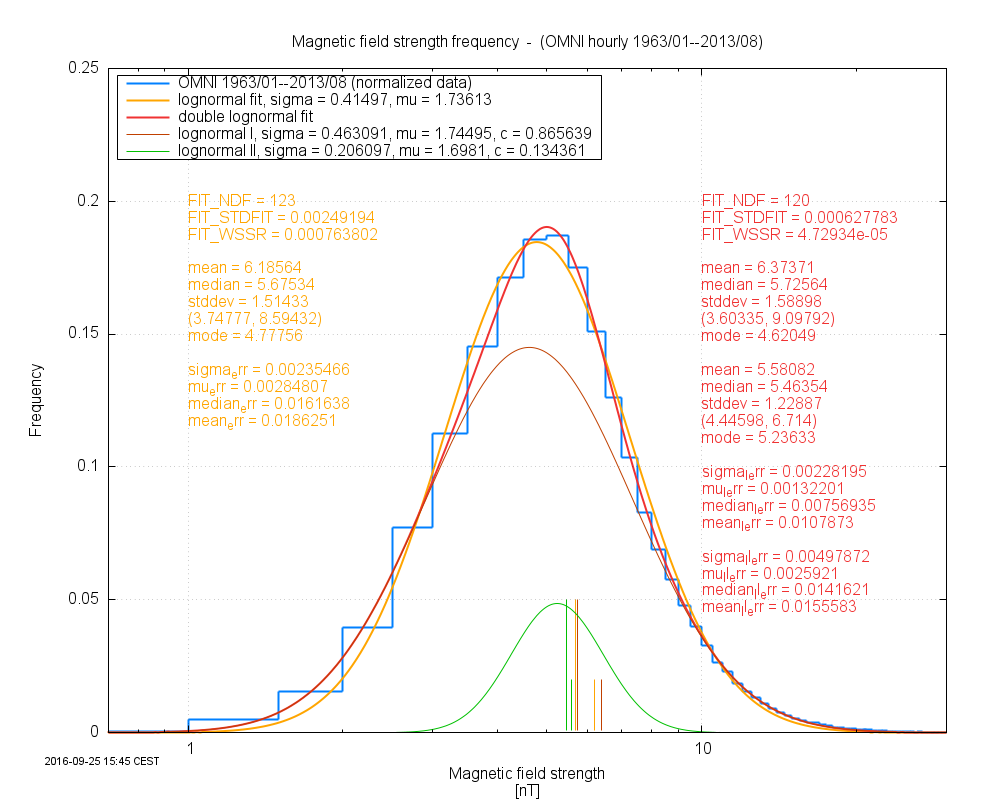
\includegraphics[width=0.3\textwidth]{images/gnuplots/histogram_B_frequency_fit_plot.png}
	}{
		\caption{Plot of the double lognormal fit on the magnetic field strength frequency distribution. 3:2}
		\label{fig:histogram_B_frequency_fit_plot_DOUBLE}
	}
\end{figure}

goodness of fit; discuss high value zoom figures\\


%goodness of fit comparison
To be able to compare the goodness of the single with the compositional lognormal fits we make use of their corresponding sum of squared residuals (SSR). More precisely the 'reduced SSR' where the SSR is divided by the number of degrees of freedom to account for the data set size and the fit function complexity (for more on SSRs see Appendix \autoref{sec:goodness_of_fit}). As anticipated, the reduced SSR values of the composed fit are considerably smaller. The evaluation of the ratio of the reduced SSRs of the respective single and double fits shows that indeed the double fits are 3.7--19.1 times more accurate (see \autoref{tab:shape_ssr_comparison}).
\begin{table}[htb]\small
	\centering
	\ttabbox{
	\captionsetup{belowskip=4pt}
	\caption{The reduced SSR for the single and the double lognormal fit and their ratio. use stdfit for comparison...}
	\label{tab:shape_ssr_comparison}
	}{
	\begin{tabular}{l S[table-figures-exponent=4] S[table-figures-exponent=4] S}
		\toprule
		Parameter	&\multicolumn{1}{c}{single SSR$_\text{red}$}	&\multicolumn{1}{c}{double SSR$_\text{red}$}	&\multicolumn{1}{c}{ratio s/d}\\
		\midrule
		Magnetic field	&7.64e-4	&4.73e-5	&16.15\\
		Velocity	&8.41e-6	&4.41e-7	&19.07\\
		Density		&3.23e-4	&8.67e-5	&3.73\\
		Temperature	&8.34e-13	&8.97e-14	&9.30\\
% 		Magnetic field strength	&7.64 \times 10^{-4}	&4.73 \times 10^{-5}	&16.15\\
% 		Velocity		&8.41 \times 10^{-6}	&4.41 \times 10^{-7}	&19.07\\
% 		Density			&3.23 \times 10^{-4}	&8.67 \times 10^{-5}	&3.73\\
% 		Temperature		&8.34 \times 10^{-13}	&8.97 \times 10^{-14}	&9.30\\
		\bottomrule
	\end{tabular}
	}
\end{table}


%discussion of comparison-table 
Especially the velocity and the magnetic field strength benefit from the more complex fit function.\\
When is the single fit sufficient? -> maybe evaluate from absolute goodness of fit...\\


\subsection{Helios solar wind model}

Helios data, radial binned and frequency binned\\
Fit on the solar distance and frequency using the balancing parameter $c$ from the compositional shape fit before (see equation~(\ref{eq:double_lognormal_fit_function})).\\
=> fit function with solar distance dependency\\
to be able to make the model's radial dependency exponential, we fit not $\mu$ and $\sigma$ but the median ($\tilde{x}, x^\text{med}, x_\text{med}, \xi$?) and mean ($\bar{x}$) of both lognormal functions to the data. As these parameters can be derived from each other directly, equation (\ref{eq:double_lognormal_fit_function}) with the replacing relations\\
\begin{align}
	\tilde{x} &= \text{e}^{\mu}	&	&\Longrightarrow	&	\mu &= \ln(\tilde{x})\\
	\bar{x} &= \text{e}^{(\mu + \frac{\sigma^2}{2})}	&	&\Longrightarrow	&	\sigma &= \sqrt{2 \ln\left(\frac{\bar{x}}{\tilde{x}}\right)}
\end{align}
results in
\begin{align}
	W_\text{II}(x,\tilde{x}_1,\bar{x}_1,\tilde{x}_2,\bar{x}_2) = \frac{c}{2 \sqrt{\pi \ln\left(\frac{\bar{x}_1}{\tilde{x}_1}\right)} \, x} \, \exp\left(- \frac{\ln^2\left(\frac{x}{\tilde{x}_1}\right)}{4 \ln\left(\frac{\bar{x}_1}{\tilde{x}_1}\right)}\right) + \frac{(1 - c)}{2 \sqrt{\pi \ln\left(\frac{\bar{x}_2}{\tilde{x}_2}\right)} \, x} \, \exp\left(- \frac{\ln^2\left(\frac{x}{\tilde{x}_2}\right)}{4 \ln\left(\frac{\bar{x}_2}{\tilde{x}_2}\right)}\right)
\end{align}
introducing the radial exponential dependency of the mean and median\\
\begin{align}
	\tilde{x}_1(r) = \tilde{a}_1 \, r^{\tilde{b}_1}\\
	\bar{x}_1(r) = \bar{a}_1 \, r^{\bar{b}_1}\\
	\tilde{x}_2(r) = \tilde{a}_2 \, r^{\tilde{b}_2}\\
	\bar{x}_2(r) = \bar{a}_2 \, r^{\bar{b}_2}
\end{align}
we get the ultimate monster equation:\\
\begin{align}
	W_\text{II}(x,\tilde{a}_1, \tilde{b}_1, \bar{a}_1, \bar{b}_1, \tilde{a}_2, \tilde{b}_2, \bar{a}_2, \bar{b}_2) =\\
	\frac{c}{2 \sqrt{\pi \ln\left(\frac{\bar{a}_1 \, r^{\bar{b}_1}}{\tilde{a}_1 \, r^{\tilde{b}_1}}\right)} \, x} \, \exp\left(- \frac{\ln^2\left(\frac{x}{\tilde{a}_1 \, r^{\tilde{b}_1}}\right)}{4 \ln\left(\frac{\bar{a}_1 \, r^{\bar{b}_1}}{\tilde{a}_1 \, r^{\tilde{b}_1}}\right)}\right) + \frac{(1 - c)}{2 \sqrt{\pi \ln\left(\frac{\bar{a}_2 \, r^{\bar{b}_2}}{\tilde{a}_2 \, r^{\tilde{b}_2}}\right)} \, x} \, \exp\left(- \frac{\ln^2\left(\frac{x}{\tilde{a}_2 \, r^{\tilde{b}_2}}\right)}{4 \ln\left(\frac{\bar{a}_2 \, r^{\bar{b}_2}}{\tilde{a}_2 \, r^{\tilde{b}_2}}\right)}\right)
\end{align}



the model represents the data well, see \autoref{fig:double_fit_B_freq_r_004au_plot_thesis}\\
\begin{figure}[htb]
	\centering
	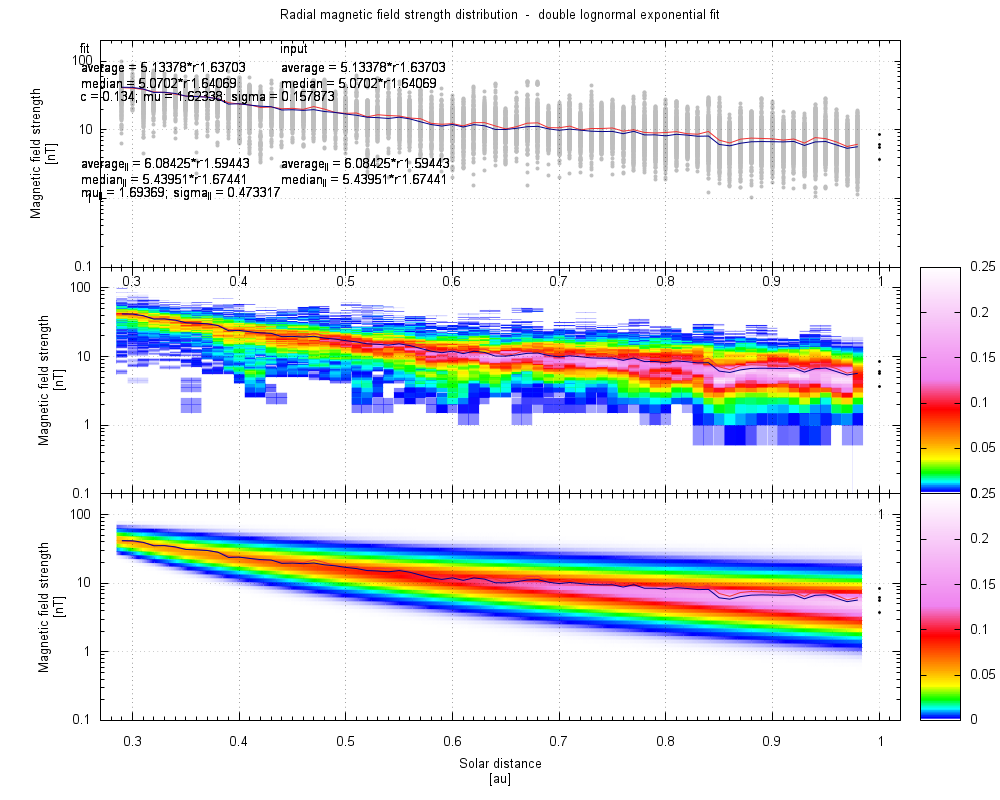
\includegraphics[width=0.4\textwidth]{images/gnuplots/double_fit_B_freq_r_004au_plot_thesis.png}
	\caption{Plot of the magnetic field strength over solar distance. The top panel shows the hourly data from both Helios spacecraft, their median and their mean values. The second panel shows the same data binned into 0.1~au and 0.5~nT bins. The bins are normalized for distance, i.e. the bin values represent the frequency of getting the bin magnitude at that distance. The bottom panel shows the exponential double lognormal function (XX), which is obtained from fitting to the data. insert keys... adjust color scale... keep log x scale?}
	\label{fig:double_fit_B_freq_r_004au_plot_thesis}
\end{figure}

The resulting fit coefficients for all four solar wind parameters are presented in \autoref{tab:helios_model_fit_parameters}.
\begin{table}[htb]\small
	\centering
	\captionsetup{belowskip=4pt}
	\caption{These are the resulting fit coefficients from the compositional function (XX). precision... Fit error in brackets? 2-line table if fit errors do not reduce it enough...}
	\begin{tabular}{lcccccccccccc}
		\toprule
		\multirow{3}{*}{Plasma parameter}	&	&\multicolumn{5}{c}{$W_1(x,r)$}	&	&\multicolumn{5}{c}{$W_2(x,r)$}\\
		\cmidrule{3-7}	\cmidrule{9-13}
			&$c$	&\multicolumn{2}{c}{median}	&	&\multicolumn{2}{c}{mean}	&	&\multicolumn{2}{c}{median}	&	&\multicolumn{2}{c}{mean}\\
		\cmidrule{3-4}	\cmidrule{6-7}	\cmidrule{9-10}	\cmidrule{12-13}
			&	&$a$	&$b$	&	&$a$	&$b$	&	&$a$	&$b$	&	&$a$	&$b$\\
		\midrule
		Magnetic field strength	&0.866	&5.43951	&-1.67441	&	&6.08425	&-1.59443	&	&5.0702	&-1.64069	&	&5.13378	&-1.63703\\
		Velocity		&0.502	&370.994	&0.114544	&	&373.556	&0.107352	&	&480.016	&-0.0151313	&	&494.135	&-0.0207186\\
		Density		&0.751	&6.75345	&-2.17915	&	&8.13399	&-2.19658	&	&3.09089	&-2.12598	&	&3.42042	&-2.08600\\
		Temperature		&0.669	&41\,262.8	&-1.18491	&	&58\,852.7	&-1.32940	&	&141\,238	&-0.570392	&	&168\,399	&-0.520731\\
% 		Plasma parameter	&$c$	&$\mu_1$	&$\sigma_1$	&$\mu_2$	&$\sigma_2$\\
% 		\midrule
% 		Magnetic field strength	&0.866	&1.69369	&0.473315	&1.62338	&0.157874\\
% 		Velocity		&0.502	&5.91619	&0.117315	&6.17382	&0.240790\\
% 		Density		&0.751	&1.91005	&0.609916	&1.12846	&0.450123\\
% 		Temperature		&0.669	&10.6277	&0.842705	&11.8582	&0.593111\\
		\bottomrule
	\end{tabular}
	\label{tab:helios_model_fit_parameters}
\end{table}

The model's amplitude differences to the data are becoming larger with smaller solar distance (check it.), see \autoref{fig:double_fit_B_freq_r_plot_thesis}\\
\begin{figure}[htb]
	\centering
	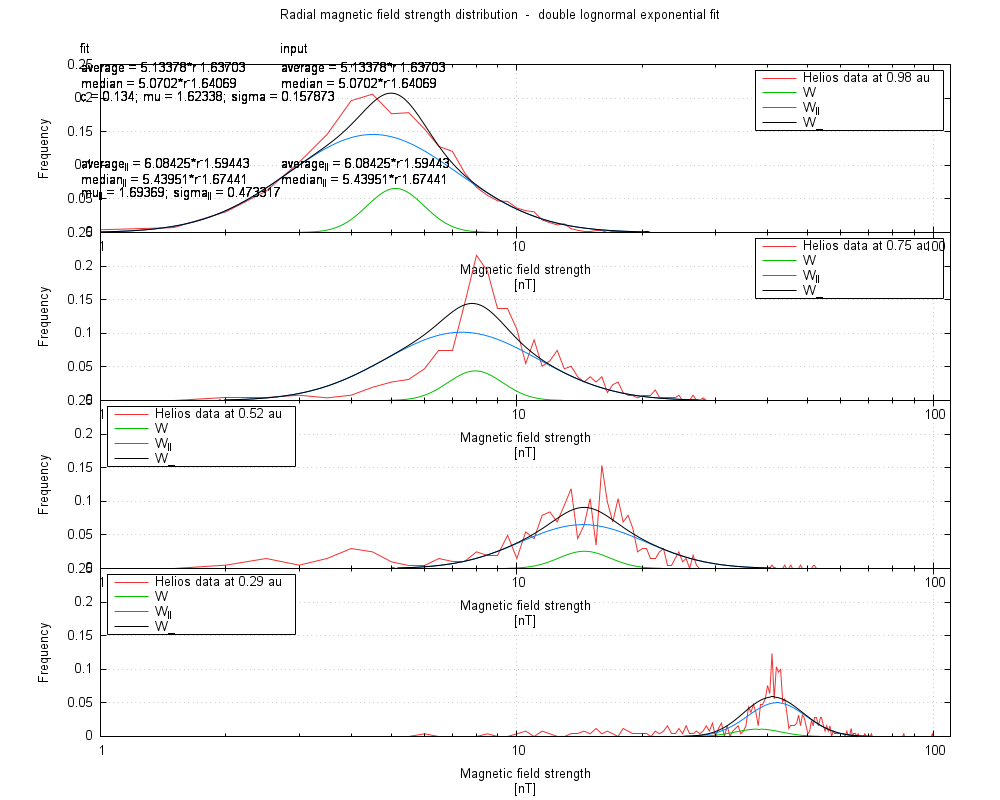
\includegraphics[width=0.4\textwidth]{images/gnuplots/double_fit_B_freq_r_plot_thesis.png}
	\caption{Plot of the magnetic field strength's frequency distribution at different solar distances (0.29, 0.52, 0.75 and 0.98~au). The Helios data, the composed fit model and both its components are plotted. 0.23~au steps, lw 2, stepfunction}
	\label{fig:double_fit_B_freq_r_plot_thesis}
\end{figure}


comparison with simple radial mean and median\\

%%%%%%%%%%%
The distribution width varies with heliospheric distance (back up with figure!).\\

We see that the density and temperature shapes stay almost constant...\\

varying shape with distance is indicator for internal physical processes (mixing/turbulence...)\\


\subsubsection{Model quality}

self-consistency?; model assumptions valid?\\

limitations: The model is valid within the heliospheric distance range of 0.29--0.98~au in the ecliptic plane (with maximal errors of...). average hourly values.\\

validity and estimation of error size outside of valid model range...\\
spatial ranges:\\
- radial range of model validity (extrapolation boundaries)\\
- latitude range...\\

Model extrapolation to near-Sun region (and Mars orbit?)\\

expanding the range of the model to the Sun leads to a singularity, see \autoref{fig:double_fit_B_freq_r_004au_plot}
\begin{figure}[htb]
	\centering
	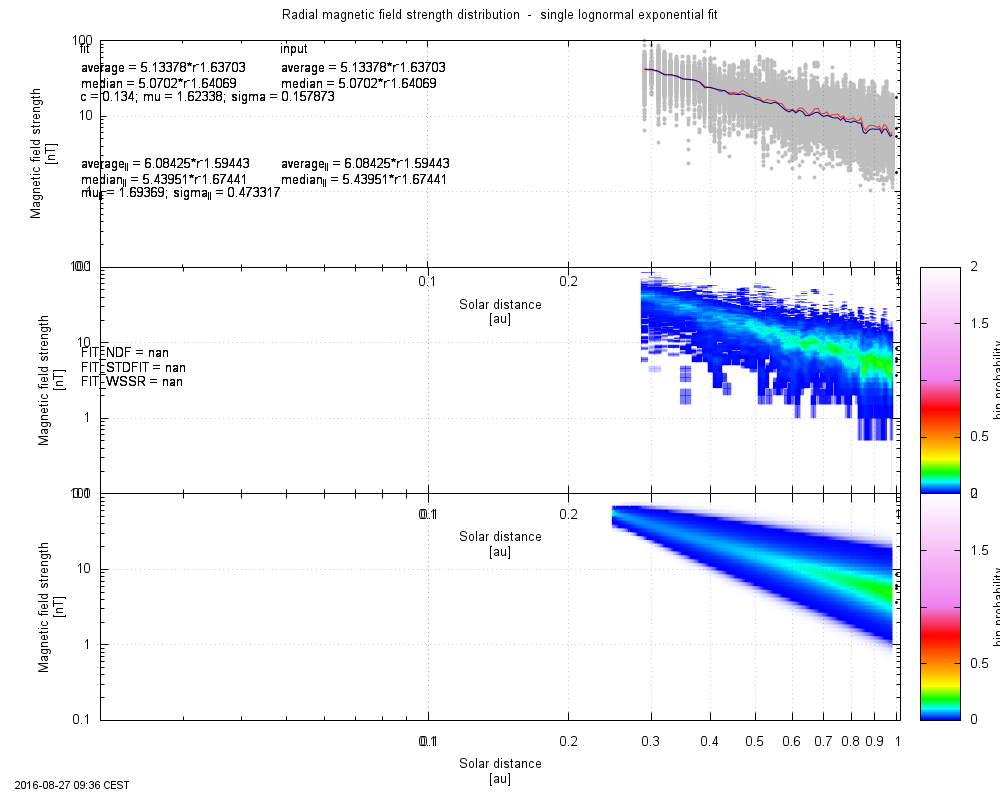
\includegraphics[width=0.4\textwidth]{images/gnuplots/double_fit_B_freq_r_004au_plot.png}
	\caption{expanding the range of the model to the Sun leads to a singularity... expand range to >2~au...}
	\label{fig:double_fit_B_freq_r_004au_plot}
\end{figure}
that is caused by the convergence and eventually crossing of median(r) and mean(r)\\

%argument for constant width function
for the magnetic field strength the mean and median cross each other at 0.246~au. below that point it cannot be lognormally distributed anymore, because for lognormal functions always applies mean > median (see Section~XX)\\
=> what kind of distribution has the B-field near the Sun?\\

%crossing distances:
% B: W1: 0.246466~au\\
% W2: 0.0332098\\
% v: W1: 2.603616\\
% W2: 179.1872517\\
% n: W1: 43094.3434\\
% W2: 0.0793510\\
% T W1: 11.674953\\
% W2: 0.0289609\\

\section{Extrapolation model}

for the extrapolation it is better to use a single lognormal function, because:\\
- extrapolation error so big that additional accuracy would not matter\\
- [easier to compute the mean(r) and median(r); otherwise numerical determination]\\
- model easier to modify for different time ranges\\
- ...\\
new requirement: possibility to extrapolate the model to the near-Sun region\\
to avoid the crossing of median(r) and mean(r), their exponents $b$ have to be identical (constant width)\\
$median(r) = X_{\text{med},0} r^b$\\
$mean(r) = mean_0 r^b$\\
fit function here...\\
So the new fit function has only the three fit parameters $median_0, mean_0$ and $b$.\\

The resulting fit coefficients for all solar wind parameters are presented in \autoref{tab:extrapolation_model_fit_parameters}.
\begin{table}[htb]\small
	\centering
	\captionsetup{belowskip=4pt}
	\caption{The resulting fit coefficients from the single lognormal fit of function (XX). constant width... Standard fit error in brackets.}
	\begin{tabular}{l.{3.13}.{3.13}.{2.8}}
		\toprule
		Parameter	&\multicolumn{1}{c}{$\tilde{x}_0$\up{a}}	&\multicolumn{1}{c}{$\bar{x}_0$\up{a}}	&\multicolumn{1}{c}{$b$}\\
		\midrule
		Magnetic field	&5.358(25)	&5.705(28)	&-1.662(11)\\
		Velocity	&399.1(17)	&411.7(18)	&0.0711(71)\\
		Density		&5.424(33)	&6.845(47)	&-2.114(20)\\
		Temperature	&6.357(64) \times 10^4	&1.072(14) \times 10^5	&-1.100(20)\\
% 		Magnetic field	&5.35847~nT	&5.70494~nT	&-1.66152\\
% 		Velocity		&399.080~km/s	&411.699~km/s	&0.0710568\\
% 		Density			&5.42431~cm$^{-3}$	&6.84454~cm$^{-3}$	&-2.11388\\
% 		Temperature		&63\,570.7~K	&107\,224~K	&-1.10001\\
% 		Magnetic field	&0.025	&0.028	&0.011\\
% 		Velocity	&1.7	&1.8	&0.0071\\
% 		Density		&0.033	&0.047	&0.015\\
% 		Temperature	&640	&1390	&0.020\\
		\bottomrule
		\multicolumn{4}{l}{\footnotesize{\up{a}Values in their respective units nT, km/s, cm$^{-3}$ and K.}}
	\end{tabular}
	\label{tab:extrapolation_model_fit_parameters}
\end{table}

frequency distribution, see \autoref{fig:single_fit_B_freq_r_plot_const_width}
\begin{figure}[htb]
	\centering
	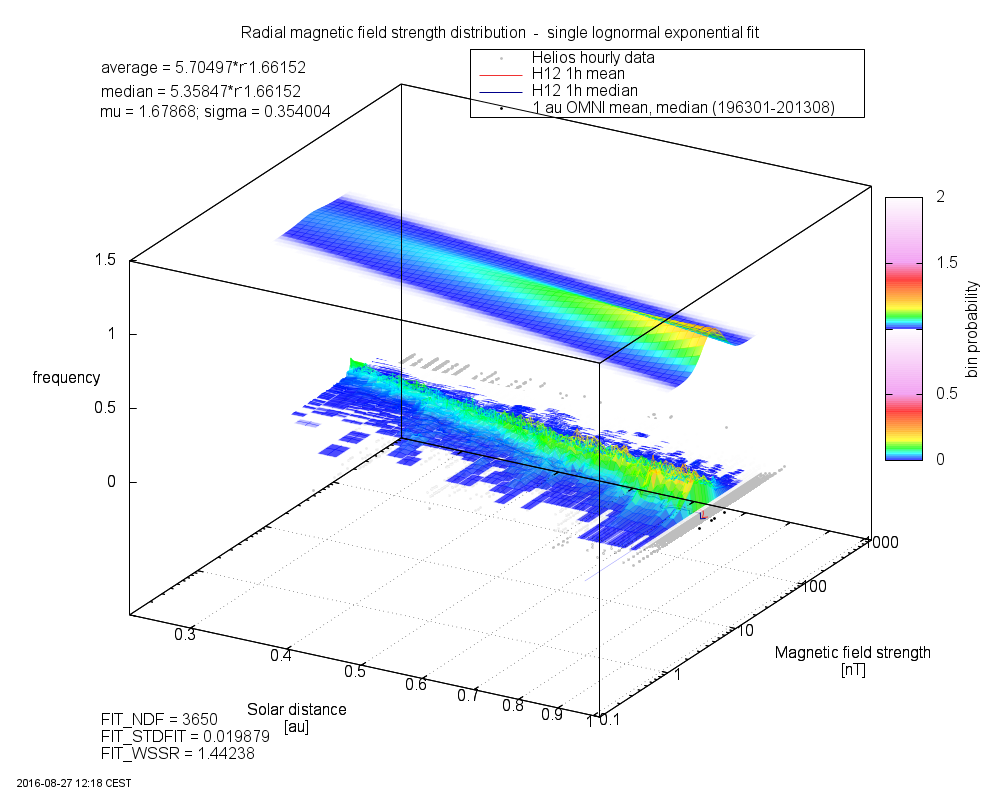
\includegraphics[width=0.4\textwidth]{images/gnuplots/single_fit_B_freq_r_plot_const_width.png}
	\caption{remove 3d plot, make 2d Plot of the magnetic field strength's frequency distribution at different solar distances (0.29, 0.52, 0.75 and 0.98~au). The Helios data and the single lognormal fit model with constant width are plotted. 0.23~au steps, stepfunction}
	\label{fig:single_fit_B_freq_r_plot_const_width}
\end{figure}

single fit model with constant width, see \autoref{fig:single_fit_fixed_4_thesis_plot}
\begin{figure}[htb]
	\centering
	\includegraphics[width=0.4\textwidth]{images/gnuplots/single_fit_fixed_4_thesis_plot.pdf}
	\caption{The solar wind parameter's frequency distribution over solar distance. The Helios data and the single lognormal fit model with constant width are plotted.}
	\label{fig:single_fit_fixed_4_thesis_plot}
\end{figure}

%error discussion
W error\\
B stdfit error: 0.020\\
B error at (1~au,Bmean): 0.011\\
B error at (1~au,Bmedian): 0.011\\
max data $-$ model deviation: 0.011\\

see \autoref{fig:single_fit_B_freq_r_004au_plot_const_width}
\begin{figure}[htb]
	\centering
	\includegraphics[width=0.4\textwidth]{images/gnuplots/single_fit_B_freq_r_004au_plot_const_width.png}
	\caption{Plot of the magnetic field strength over solar distance (similar to Figure~XX). The top panel shows the same data binned into 0.1~au and 0.5~nT bins. The bins are normalized for distance, i.e. the bin values represent the frequency of getting the bin magnitude at that distance. The bottom panel shows the exponential single lognormal function (XX) with constant width, which is obtained from fitting to the data. insert keys... adjust color scale... keep log x scale? remove top panel...}
	\label{fig:single_fit_B_freq_r_004au_plot_const_width}
\end{figure}

quartile fit extrapolation...\\

expected values at 0.04~au...\\


\subsection{Model validity}

validity and estimation of error size outside of valid model range...\\

The extrapolation distance is only about one third of the model range, but as the parameters follow exponential change, one has to look at the logarithmic distance which is indeed one and a half times the model range.\\

argument with gravitational deceleration; near-Sun extrapolation should be biased, because in the near-Sun region gravitation becomes significant (see \autoref{fig:v_vs_r_b})\\
\begin{figure}[htb]
	\centering
	\includegraphics[width=0.3\textwidth]{images/gnuplots/v_vs_r_b.png}
	\caption{velocity over solar distance; gravitational deceleration. place instead figure of grav. force over solar distance...}
	\label{fig:v_vs_r_b}
\end{figure}

polar plot with highlighted model range and 1-3 extrapolation extensions... (for both models)\\


\subsection{Model comparison via SSR}

model comparison via the reduced SSR for the fit parameters from Tables~\ref{tab:extrapolation_model_fit_parameters} and \ref{tab:helios_model_fit_parameters}, see \autoref{tab:model_ssr_comparison}\\
\begin{table}[htb]\small
	\centering
	\captionsetup{belowskip=4pt}
	\caption{The reduced SSR for the Helios model and the extrapolation model fits and their ratio. precision...}
	\begin{tabular}{l>{$}l<{$}>{$}l<{$}c}
		\toprule
		Plasma parameter	&$Helios model $SSR_\text{red}	&$Extrapolation model $SSR_\text{red}	&ratio Helios/extrapolation\\
		\midrule
		Magnetic field strength	&1.18			&1.44			&1.22\\
		Velocity		&2.66 \times 10^{-3}	&3.47 \times 10^{-3}	&1.30\\
		Density			&2.54 \times 10^{-1}	&2.67 \times 10^{-1}	&1.05\\
		Temperature		&2.14 \times 10^{-9}	&2.35 \times 10^{-9}	&1.10\\
% 		Magnetic field strength	&1.17979		&1.44238		&1.223\\
% 		Velocity		&2.66309 \times 10^{-3}	&3.47353 \times 10^{-3}	&1.304\\
% 		Density			&0.254132		&0.26671		&1.049\\
% 		Temperature		&2.13713 \times 10^{-9}	&2.34673 \times 10^{-9}	&1.098\\
		\bottomrule
	\end{tabular}
	\label{tab:model_ssr_comparison}
\end{table}


\subsection{Adjusted extrapolation models}

extrapolation models for different time spans:\\
extrapolation with OMNI data and solar cycle/seasonal variations\\


\subsection{Comparison with existing extrapolation models}

comparison with s.o. elses values...\\
...with Vourlidas estimates at 10~$R_\odot$\\
...with Wang2000 slow blobs\\


\section{Radial evolution of solar wind structures}

%see CGAUSS report2015_2

Radial evolution of solar wind structures from Helios data\\

Helios event lists HSSs, SLOWs, CIRs, CMEs...; event lists for all Helios data\\
see Liu2004 for Helios ICME list and radial dependencies of B, n, T and v...\\

200~km/s slow solar wind at 10~$R_\odot$ is in agreement with blob measurements from Wang2000\\

very slow sw (VSSW) gets accelerated; see Sanchez-Diaz2016:\\
%"The reported in situ measurements suggest that the properties of VSSW are a continuation of the slow wind toward lower speeds: higher densities, higher proton fluxes, and lower temperatures, thereby extending well-known scaling laws [Lopez and Freeman, 1986; Hundhausen et al., 1970] down to speeds as low as 200 km/s."\\
%"The VSSW has a number of interesting properties that suggest it may be the interplanetary signature of long HPS crossings."\\

structure extrapolations\\

radial diameter of MCs increase between 0.3~au and 4.3~au proportional to the distance as $r^{0.8}$ \citep{Bothmer1998}\\

MC central axial magnetic field strength radial density dependence $B = 18.1\,r^{-1.64}$ \citet{Leitner2007}\\
MC average diameter $D = 0.23\,r^{1.14}$ \citet{Leitner2007}

sw structure marked plot\\


\section{Summary/Results}

where does the solar wind get accelerated? (at 3--4~Rs for moving density enhancements (slow solar wind), see Sheeley1997)\\
results beneficial for Solar~Probe~Plus (SPP) mission which is to investigate coronal heating and the origin of the solar wind\\
SPP will have its closest perihelion at 9.86~solar radii (0.0459~au), see \citet{Fox2015}\\

	\chapter[Discussion and results]{Discussion/conclusions/results}
%\label{chap:}

%COFI -- chapter outline and flow integration\\

discussion\\
conclusions\\
results\\

Prediction:\\
Link from near-Sun solar wind measurements to Kp impact\\
Link from near-Sun structure (CMEs, CIRs) measurements to Kp impact\\

	\chapter{Summary and outlook}
%\label{chap:}

%COFI -- chapter outline and flow integration\\

Outlook\\
DSCOVR data (advantages over ACE? gain?)\\
anticipated Solar~Probe~Plus data (near-Sun data)\\

other possible space weather missions: sub-L1 (earlier in situ CME magnitude warning) and L5 (early CME velocity and arrival warning)

%SPP orbit:	1.09 SPP orbit presentation-Lario.ppt

I built an empirical solar wind model for the ecliptical inner heliosphere which accounts for variations in time (season and solar cycle) and space (solar distance).\\

Using the SSN prediction the model allows the forecast and extrapolation of the solar wind, which will occur during the SPP mission's first near-Sun perihela in mid"~2018.\\

%german version of summary


	%summary and conclusions

	\appendix
	\chapter{Physics}
\label{chap:physics}

\section{Electromagnetism}	%maybe exclude this section?

Electromagnetism is one of the four fundamental forces at the common level of energy. In all situations examined in this thesis (sw plasma, magnetosphere) it is by far the strongest force and the others can be neglected.\\

%Lorentz force law as the definition of E and B\\
%The electromagnetic force F on a test charge at a given point and time is a certain function of its charge q and velocity v, which can be parameterized by exactly two vectors E and B, in the functional form: (wiki)\\
The Lorentz force: $\textbf{F} = q (\textbf{E} + \textbf{v} \times \textbf{B})$\\

The Maxwell equations in differential notation:
\begin{align}
	\text{div}\,\textbf{B} &= 0\\
	\text{div}\,\textbf{D} &= \rho\\
	\text{rot}\,\textbf{H} &= \textbf{j} + \dot{\textbf{D}}\\
	\text{rot}\,\textbf{E} &= - \dot{\textbf{B}}
\end{align}
With the magnetic flux density \textbf{B} (aka magnetic field), the electric displacement field \textbf{D}, the charge density $\rho$, the magnetic field \textbf{H}, the electric field \textbf{E} and the current density \textbf{j}.\\
%note about B naming convention within this work as magnetic field strength% maybe put into beginning...


\section{Solar wind pressures}

The magnetic energy density $w_\text{mag}$ is also the magnetic pressure $p_\text{mag}$
\begin{align}
	w_\text{mag} &= p_\text{mag}\\
	&= \frac{B^2}{2 \mu_0}	\text{\,.}
\end{align}

dynamic pressure $p_\text{dyn} = \rho v^2$\\
thermal pressure $p_\text{therm} = n k_\text{B} T$\\
magnetic pressure $p_\text{mag} = B^2 / (2 \mu_0)$ (see above...)\\
ram pressure??\\
%VB1998p104


\section{Plasma beta}	%Plasma beta formula
In MHD the magnetic energy density behaves like an additional pressure that adds to the gas pressure of a plasma (Wikipedia; find alternative source...).

The ratio of the thermal pressure $p = n k_\text{B} T$ to the magnetic pressure $p_\text{mag} = \frac{B^2}{2 \mu_0}$ is called plasma beta
\begin{align}
	\beta &= \frac{p}{p_\text{mag}}\\
	&= \frac{2 \mu_0 n k_\text{B} T}{B^2}
\end{align}
with the number density $n$.\\
$\beta \ll 1$: ``cold'' plasma; magnetic field contains plasma (magnetic clouds)\\
$\beta \geq 1$: ``warm'' plasma; plasma keeps magnetic field

%aka proton beta
plasma beta see \citep[p.~50]{Kivelson1995}

typical $beta$-values for solar wind are in the range X--Y.\\

% Plasma beta:\\
% near-sun β << 1:\\
% far-sun β ≥ 1:\\
% β = p /pkin mag\\
% plasma follows magnetic field\\
% magnetic field is frozen within plasma\\
% --> spiral-like B-field\\
% Bφ ≈ -45° @ 1 au\\


\section{Alfv\'en waves}	%Alfv\'en velocity
%maybe MHD waves

named after Hannes~Alfv\'en...

There exists an incompressible wave mode which is a result of bending magnetic field lines called shear Alfv\'en wave.

In an ideal incompressible MHD plasma (viscosity $\mu = 0$ and electrical conductivity $\sigma = \infty$) the kinetic and magnetic energy density are of equal value: 
\begin{align}
	w_\text{kin} &= w_\text{mag}\\
	\frac{\rho v^2}{2} &= \frac{B^2}{2 \mu_0}	\nonumber
\end{align}
with the permeability constant
\begin{align}
	\mu_0 &= 4 \pi \cdot \SI{e-7}{\newton\per\ampere\squared}	\nonumber
	%&\approx \SI{1.25663e-6}{\newton\per\ampere\squared}
\end{align}
and the total mass density $\rho$ of the charged plasma particles.

So waves propagate with the so-called Alfv\'en velocity
\begin{align}
	v_\text{A} = \frac{|B|}{\sqrt{\mu_0 \rho}}	\text{\,.}
\end{align}
Their phase velocity is
\begin{align}
	v_\text{ph} = v_\text{A} \cos(\theta)
\end{align}
with $\theta$ the angle between wave propagation direction (k) and magnetic field line (B). => Alfv\'en waves travel along magnetic field lines. Alfv\'en waves are characterized by periodic disturbances in the magnetic field perpendicular to its direction, in the electric field, in the plasma velocity and in the current density. They do not affect the plasma density, plasma pressure and magnetic field magnitude.

Additionally, there exist two types of compressional waves within MHD plasmas, the fast-mode wave and the slow-mode wave. The phase speeds of the three MHD waves meet $v_\text{fast} \geq v_\text{A} \geq v_\text{slow}$. %block copy from Kivelson1995

Alfv\'en waves are dominant in regions that are open to the heliosphere. %copy from Cranmer2005 p.1\\

Alfv\'en waves see \citep[pp.~51ff.]{Kivelson1995}\\


Within average solar wind at 1\,au their typical frequency is 1--4 per hour (cite?) ($v_\text{A} = 53$~km/s for $B = 5.6$~nT and $\rho = 5.3$~cm$^{-3}$).

critical surfaces, solar wind acceleration...\\

%wolfram alpha:
%solve v = 0.001*B/sqrt(mu*rho), B=5.6*10^-9, rho=5.3*10^6*1.66*10^-27, mu=4*pi*10^-7

%v_A=53.3km/s for r=1au; B=5.6nT; N=5.3cm-3
%v_A=91.5km/s for r=0.3 au; B=37.9nT; N=82.2cm-3
%v_A=280.6km/s for r=0.04 au; B=930.6nT; N=5274cm-3

%slow wind: v_A=28.5km/s for r=1au; B=4.7nT; N=13.0cm-3
%fast wind: v_A=68.7km/s for r=1au; B=5.7nT; N=3.3cm-3

%Cranmer2005 - ON THE GENERATION, PROPAGATION, AND REFLECTION OF ALFVÉN WAVES FROM THE SOLAR PHOTOSPHERE TO THE DISTANT HELIOSPHERE


\section{Solar rotation}
\label{sec:solar_rotation}

%rotation period
%surface differential rotation
%rotation axis tilt
the rotation was first discovered from sunspots in 18XX?

\citet{Bartels1934} set the synodic solar rotation period to 27~days for the definition of his solar rotation number. The Bartels' Rotation Number counts the solar rotations starting with 8 February 1832.\\
Carrington solar rotation period of 27.2753~days (Where Carrington Rotation Number is based upon, starting with November 9, 1853; Wikipedia...)\\
%synodic rotation period of 27.2753 days (or a sidereal period of 25.38 days; This chosen period roughly corresponds to rotation at a latitude of 16~deg (sic), which is consistent with the typical latitude of sunspots and corresponding periodic solar activity; cite from https://en.wikipedia.org/wiki/Solar_rotation

Solar surface rotation period at 16\degree{} latitude:\\
sidereal: 25.38~d (of 609.12~h Sun Fact Sheet...), synodic: 27.2753~d (derived)\\


\subsection{Solar surface differential rotation}
\label{sec:solar_surface_differential_rotation}

The Sun's inner thermal convective circulation results in a differential rotation caused by transport of angular momentum away from the rotation axis.

%best-fitting function
The Sun's sidereal differential angular velocity best-fitting function with values as stated in (Sun~Fact~Sheet...)\footnote{NASA's \textit{Sun~Fact~Sheet} (\url{http://nssdc.gsfc.nasa.gov/planetary/factsheet/sunfact.html}, accessed 2016-08-19).} is
\begin{align}
	\omega_\odot = A + B \sin^2(b) + C \sin^4(b)
\end{align}
with the latitude $b$, the equatorial angular velocity $A = 14.37$\textdegree/d, the coefficients $B = -2.33$\textdegree/d and $C = -1.56$\textdegree/d (see \autoref{fig:differential_rotation_pdfcairo_plot}).

see \autoref{fig:differential_rotation_pdfcairo_plot}
\begin{figure}[htb]
	%\centering
	\fcapside[\FBwidth]{
		\includegraphics[width=0.5\textwidth]{images/gnuplots/differential_rotation_pdfcairo_plot.pdf}
	}{
		\caption{Diagram of the sidereal solar surface differential rotation. It shows the angular velocity for different latitudes.}
		\label{fig:differential_rotation_pdfcairo_plot}
	}
\end{figure}

\noindent Thus, the solar equatorial rotation period (sidereal) is
\begin{align}
	T_\odot^\text{eq} &= 360\degree / A\\
	&= 25.05~\text{d}	\nonumber\\
\shortintertext{and the synodic period is}
	T_\odot^\text{eq,syn} &= 1/(1/T_\odot^\text{eq} - 1/T_\text{Earth})\\
	&= 26.90~\text{d}	\nonumber
\end{align}
with the Earth's orbital rotation period $T_\text{Earth} = 365.25$~d (1/100 Julian century).\\

Solar surface rotation period at equator\\
sidereal: 25.05~d (Sun Fact Sheet...), synodic: 26.90~d (derived)\\
Solar surface rotation period at poles:\\
sidereal: 34.35~d (diff. rot. formula), synodic: 37.92~d (derived)\\
are listed in \autoref{tab:solar_surface_rotation_periods}.\\
\begin{table}[htb]\small
	\centering
	\captionsetup{belowskip=4pt}
	\caption{Solar surface rotation periods for equator, \SI{+-16}{\degree}~latitude and poles (sidereal and synodic).}
	\begin{tabular}{llll}
		\toprule
				&Equator	&\SI{+-16}{\degree}~latitude	&Poles\\
				&\multicolumn{1}{c}{[d]}	&\multicolumn{1}{c}{[d]}	&\multicolumn{1}{c}{[d]}\\
		\midrule
		Sidereal	&25.05	&25.38	&34.35\\
		Synodic	&26.90	&27.2753$^\text{a}$	&37.92\\
		\bottomrule
		\multicolumn{4}{l}{\footnotesize{$^\text{a}$Carrington solar rotation period}}
	\end{tabular}
	\label{tab:solar_surface_rotation_periods}
\end{table}


%meridional flow

The meridional circulation is the proposed equatorial updrift and polar downdrift - a result of Reynolds stress and convective transport (cite?).\\


\subsection{Solar rotation axis tilt}
%\label{sec:}

The inclination of the solar equator to the ecliptic (tilt/obliquity) is $i_\odot = 7.25$\textdegree{} \citep{USNO2015}. %C3

Viewed from Earth the projected solar rotation axis tilt angle varies as the Earth is moving on its orbit.\\

At the time XX the angle is zero.\\

The projected tilt angle to Earth over the year is\\

% Stonyhurst disk
% 
% Calculation of solar tilt angle at given time
% solar tilt/obliquity to ecliptic: i_sun = 7.25\degrees (Sun fact sheet: \url{http://nssdc.gsfc.nasa.gov/planetary/factsheet/sunfact.html)}
% modulate this angle with a sine over the year:
% projected tilt from Earth: i_proj = i_sun * sin(beta)
% this years vernal equinox: eq = 2015.0 + 2.0/12.0 + 20.0/365.0 = 2015.2215
% actual separation angle from vernal equinox position: phi = (today - eq) * 360
% 
% ecliptic longitude: \url{http://cohoweb.gsfc.nasa.gov/helios/plan_des.html}
% Ecliptic longitude of ascending node of the Sun's equator
% http://sspg1.bnsc.rl.ac.uk/SEG/Coordinates/angles.htm

%Hapgood (1992), Space Physics Coordinate Transformations: A User Guide
\citet{Hapgood1992}:
\begin{align}
	\omega = 73.67 + 0.013\,958 * (today - 1850.0)	%#why? yearly change
\end{align}
% beta = phi - omega
% 
% Meridians (longitude lines)
% 
% Parallels (latitude lines)


% vernal_equinox = 2016.0 + 2.0/12.0 + 20.0/366.0
% tilt(x) = 7.25 * sin(-(73.67 + 0.013958 * (x - 1850.0)) + (-vernal_equinox + x) * 360.0)
% 
% 	tilt(2016.0+(x-1.0)/12.0) with lines title "sine approx." ls 2 lw 2,\

solar tilt over the year, see \autoref{fig:Solar_tilt_seasons_plot}
\begin{figure}[htb]
	%\centering
	\fcapside[\FBwidth]{
		\includegraphics[width=0.5\textwidth]{images/gnuplots/Solar_tilt_seasons_plot.pdf}
	}{
		\caption{Projected solar tilt angle over the year as viewed from Earth. remove sides...}
		\label{fig:Solar_tilt_seasons_plot}
	}
\end{figure}


\section{Coordinate systems}
\label{sec:coordinate_systems}

Coordinate systems used in this thesis:\\
GSE - Geocentric Solar Ecliptic\\
GSM - Geocentric Solar Magnetospheric\\
%RTN - Radial Tangential Normal\\
%SE - Solar Ecliptic\\
%SSE - Sun-centered Solar Ecliptic\\
HGI - Heliographic Inertial\\

refer to \citet{Hapgood1992} for GSE and GSM\\

figures for GSE and GSM

% RTN - Radial Tangential Normal
%     Spacecraft centered coordinate system. 
%     R = Sun to Spacecraft unit vector 
%     T = (Omega x R) / | (Omega x R) |
%         where Omega is Sun's spin axis (in J2000 GCI)
%     N completes the right-handed triad

%R is a unit vector pointing from the Sun to the spacecraft. T is Omega x R, where Omega is a unit vector along the Sun's rotation axis. N = R x T.

% The RTN system is fixed at a spacecraft (or the planet). The R axis is directed
% radially away from the Sun, the T axis is the cross product of the solar
% rotation axis and the R axis, and the N axis is the cross product of R and T. 
% At zero Heliographic Latitude when the spacecraft is in the solar equatorial
% plane the N and solar rotation axes are parallel.
%source: http://cdaweb.gsfc.nasa.gov/misc/NotesU.html#UY_COHO1HR_MERGED_MAG_PLASMA
  
%http://omniweb.sci.gsfc.nasa.gov/coho/helios/plan_des.html
%Solar Ecliptic Coordinate System (SE)
%The SE is a heliocentric coordinate system with the Z-axis normal to and northward from the ecliptic plane. The X-axis extends toward the first point of Aries (Vernal Equinox, i.e. to the Sun from Earth in the first day of Spring). The Y-axis completes the right handed set. The Vernal Equinox direction changes slowly; commonly invoked equinox epochs are (1) B-1950, (2) Mean-of-(current) Date, and (3) J-2000. The ecliptic longitude SE_LONG increases from zero in the x-direction towards Y-direction; the latitude, SE_LAT increases to +90 deg towards north ecliptic pole and to -90 deg towards south pole.These Lat/Long are designated as ELAT and ELON in output.

%SSE - Sun-centered Solar Ecliptic coordinates

%HGI - Heliographic Inertial coordinates
%The HGI coordinates are Sun-centered and inertially fixed with respect to an X-axis directed along the intersection line of the ecliptic and solar equatorial planes, and defines zero of the longitude, HGI_LONG. The solar equator plane is inclined at 7.25 degrees from the ecliptic. This direction was towards ecliptic longitude of 74.367 deg on 1 January 1900 at 12:00 UT; because of the precession of the Earth's equator, this longitude increases by 1.4 deg/century. The Z-axis is directed perpendicular to and northward of the solar equator, and the Y-axis completes the right-handed set. The longitude, HGI_LONG increase from zero in the X-direction towards Y-direction.The latitude HG_LAT increases to +90 deg towards the north pole, and to -90 deg towards south pole.These Lat/Long are designated as HLAT & HILON in output

% The Heliographic Inertial (HGI) coordinates are Sun-centered and inertially
% fixed with respect to an X-axis directed along the intersection line of the
% ecliptic and solar equatorial  planes. The solar equator plane is inclined at
% 7.25 degrees from the ecliptic. This direction was towards ecliptic longitude of
% 74.36 degrees  on  1  January  1900  at  1200  UT; because of precession of the
% celestial equator, this longitude increases by 1.4 degrees/century. The Z axis
% is directed perpendicular and northward from the solar equator, and the Y-axis
% completes the right-handed set. This system differs from the usual heliographic
% coordinates (e.g. Carrington longitudes) which are fixed in the frame of the
% rotating Sun.
%source: http://cdaweb.gsfc.nasa.gov/misc/NotesU.html#UY_COHO1HR_MERGED_MAG_PLASMA


\subsection{Geocentric Solar Ecliptic}
\label{sec:geocentric_solar_ecliptic}

The Geocentric Solar Ecliptic (GSE) coordinates are\\
GSE - Geocentric Solar Ecliptic\\
    X = Earth-Sun Line\\
    Z = Ecliptic North Pole

GSE coordinates are used in ACE solar wind data, etc.

%http://www.srl.caltech.edu/ACE/ASC/coordinate_systems.html
%https://www.spenvis.oma.be/help/background/coortran/coortran.html
%http://adsabs.harvard.edu/abs/1992P%26SS...40..711H


\subsection{Geocentric Solar Magnetospheric}

GSM - Geocentric Solar Magnetospheric\\
X = Earth-Sun Line\\
Z = Projection of dipole axis on GSE YZ plane\\
%(Z-axis (positive) is perpendicular to the X-axis and parallel to the projection of the negative dipole moment on a plane perpendicular to the X-axis (the northern magnetic pole is in the same hemisphere as the tail of the magnetic moment vector).)\\

GSM is defined with a time dependent dipole axis.\\
the dipole axis orientation changes over time; at 1995 the northern pole was at $l = 288.59\degree$ and $b = 79.30\degree$; more recent year (2015)?... cite?\\
% https://www.spenvis.oma.be/help/background/coortran/coortran.html#MAG

\subsection{Heliographic Inertial}

HGI - Heliographic Inertial coordinates\\


\section{Earth orbit geometry}

%all from https://en.wikipedia.org/wiki/Earth's_orbit
%see also http://nssdc.gsfc.nasa.gov/planetary/factsheet/earthfact.html
Earth orbit parameters (cite?):\\
semimajor axis: $a = 1.000001018$~au\\
eccentricity: $e = 0.0167086$~au\\
%perihelion, point on solar orbit with minimum distance to Sun\\
%aphelion, point on solar orbit with maximum distance to Sun\\
distance at perihelion: (formula cite?, accuracy?)\\
\begin{align}
	r_\text{p} &= a (1 - e)\\
		&= 0.98329~\text{au}	\nonumber
\end{align}
distance at aphelion:\\
\begin{align}
	r_\text{p} &= a (1 + e)\\
		&= 1.0167~\text{au}	\nonumber
\end{align}

for calculation of heliospheric distance see HORIZONS Web-Interface at \url{http://ssd.jpl.nasa.gov/horizons.cgi}

perihelion/aphelion times...
%http://aa.usno.navy.mil/data/docs/EarthSeasons.php

\subsection{Sun tilt}
\subsection{Earth tilt}
\subsection{seasonal distance}
	%theory & calculations
	\chapter{Math}
\label{chap:math}

%in the end: sort sections in order of reference in work


\section{Correlations}
\label{sec:correlations}

auto correlation

cross correlation\\
Pearson linear correlation\\
Spearman rank correlation

Correlation in Linear Regression: \url{http://www.stat.yale.edu/Courses/1997-98/101/correl.htm}\\


\section{Lognormal distribution}
\label{sec:lognormal_distribution}

This is a small summary about the lognormal probability distribution \citep[p.~780]{Bronstein2000}. The lognormal distribution is the distribution of a random variable $X$ if the logarithm of $X$ conforms to a normal distribution. Its shape is highly asymmetric, however in a semi-log plot the Gaussian bell curve is recognizable (see the second panel of \autoref{fig:lognormal_3panel_pdfcairo_plot}).
\begin{figure}[htb]
	%\centering
	\fcapside[\FBwidth]{
		\includegraphics[width=0.5\textwidth]{images/gnuplots/lognormal_3panel_pdfcairo_plot.pdf}
	}{
		\caption{The lognormal probability density function ($\sigma = 1, \mu = 0$) plotted in a linear, semi-log and log-log way.}
		\label{fig:lognormal_3panel_pdfcairo_plot}
	}
\end{figure}
Its probability density function is
\begin{align}
	f(x) &= \frac{1}{\sigma \sqrt{2 \pi} x} \, \text{e}^{- \frac{(\ln x - \mu)^2}{2 \sigma^2}}
\end{align}
with the location ($\mu$) and the shape parameter ($\sigma$). Changes in $\mu$ affect both the horizontal and vertical scaling of the function, whereas $\sigma$ has an influence on its shape (see \autoref{fig:lognormal_ms_pdfcairo_plot}).\\
\begin{figure}[htb]
	\centering
	\includegraphics[width=0.5\textwidth]{images/gnuplots/lognormal_ms_pdfcairo_plot.pdf}
	\caption{Five lognormal distributions plotted with fixed $\sigma$ (top) and fixed $\mu$ (bottom).}
	\label{fig:lognormal_ms_pdfcairo_plot}
\end{figure}

Because it is a probability distribution, its area is normalized
\begin{align}
	\int_0^\infty f(x) \text{d} x = 1\,.
\end{align}

For a lognormally distributed random variable the geometric moments mean, standard deviation and variance are:
\begin{align*}
	&\mu_\text{g} = \text{e}^\mu ,\\
	&\sigma_\text{g} = \text{e}^\sigma ,\\
	&var_\text{g} = \text{e}^{\sigma^2}~~(!) .
\end{align*}

Its arithmetic moments are:
\begin{align*}
	&\mu_\text{a} = \text{e}^{\mu + \frac{\sigma^2}{2}} ,\\
	&\sigma_\text{a} = \text{e}^{\mu + \frac{\sigma^2}{2}} \, \left(\text{e}^{\sigma^2} - 1\right) ,\\
	&var_\text{a} = \sigma_\text{a}^2 .
\end{align*}

Other useful characteristics are the median and the mode
\begin{align*}
	&x_\text{median} = \text{e}^{\mu},\\
	&x_\text{mode} = \text{e}^{\mu - \sigma^2}\,.
\end{align*}
Note that for the lognormal distribution its median is equal to its geometric mean.\\

Applications of lognormal distributions...\\
%Limpert2001: Lognormal Distributions across the Sciences: Keys and Clues
%http://bioscience.oxfordjournals.org/content/51/5/341.full

Most natural quantities which can only be positive are lognormally distributed. e.g. animal body sizes?, animal life expectancies, financial stock prices...; income distributions.\\

%life expectancy analyses of economic, technical and biological processes. Bronstein2000


\section{Goodness of fit}
\label{sec:goodness_of_fit}

%figure with fit residuals here
$SSR$ -- sum of squared residuals\\
\begin{align}
	SSR = \sum_i (y_i - f_i)^2
\end{align}
data values $y_i$, fit function values $f_i$\\
$SSR_\text{red}$ -- reduced SSR, divided by number of degrees of freedom $\nu$\\
\begin{align}
	SSR_\text{red} = \frac{SSR}{\nu}
\end{align}
$TSS$ -- total sum of squares (in relation to the data mean)\\
\begin{align}
	TSS = \sum_i (y_i - \bar{y})^2
\end{align}
with data mean $\bar{y}$\\
%http://math.stackexchange.com/questions/1225103/whats-in-a-name-sum-of-squares
%https://en.wikipedia.org/wiki/Goodness_of_fit

$\chi^2$ -- chi-square\\
$\chi^2_\text{red}$ -- reduced chi-square, divided by number of degrees of freedom $\nu$\\

$R^2$ -- coefficient of determination\\
$0 \leq R^2 \leq 1$, ``values can be less than zero''!. if $R^2 = 1$ -> ideal fit; if $R^2 = 0$ -> bad fit
\begin{align}
	R^2 &= 1 - \frac{SSR}{TSS}
\end{align}
``In case of a single regressor, fitted by least squares, R2 is the square of the Pearson product-moment correlation coefficient relating the regressor and the response variable.'' cite from wikipedia \\%https://en.wikipedia.org/wiki/Coefficient_of_determination
%https://de.wikipedia.org/wiki/Bestimmtheitsma%C3%9F

Kolmogorov-Smirnov K-S-Test
%http://www.physics.csbsju.edu/stats/KS-test.html
%http://www.wessa.net/rwasp_Reddy-Moores%20K-S%20Test.wasp


\section{other}

%minimum variance analysis
minimum variance analysis (MVA)\\
determining magnetic cloud configuration \citep{Bothmer1998}\\

hodogramm?
%https://en.wikipedia.org/wiki/Hodograph



least-squares fit approximates mean
linear regression

robust statistics

Non-parametric inferential statistical methods are mathematical procedures for statistical hypothesis testing which make no assumptions about the probability distributions of the variables being assessed. The most frequently used tests include
- median
- percentiles (quartiles)
- Spearman's rank correlation coefficient

histogram

generalized mean
\url{http://en.wikipedia.org/wiki/Generalized_mean}



normal distribution

% inverse erf
% http://mathworld.wolfram.com/InverseErf.html
% 
% \begin{align}
% 	erfc^{-1}(x) = erf^{-1}(1 - x)
% \end{align}
% 
% quantile function: inverse cumulative distribution function (CDF) of normal distribution
% \begin{align}
% 	\mu - \sqrt{2}*\sigma*erfc^{-1}(2*x)
% \end{align}
% http://www.wolframalpha.com/input/?i=Quantile+function+normal+distribution

		%definitions, methods, calculations
	\chapter{Glossary}
\label{chap:glossary}

\section{Astronomical constants}
\label{sec:astronomical_constants}

Astronomical unit: 1~au = 149\,597\,870\,700~m \citep{USNO2015}\\ %Astronomical constants
Solar mass: $M_\odot = 1.9884(2)\times10^{30}$~kg \citep{USNO2015}\\ %see also Mamajek2015
Nominal solar radius (photosphere): $R_\odot = \SI{695700}{\km}$ \citep{Mamajek2015}\\ %Astronomical constants
Sun escape velocity: $v_\text{esc} = 617.6$~km/s (Sun Fact Sheet...)\\
Solar rotation axis tilt: $i_\odot = 7.25$\textdegree{} \citep{USNO2015}\\ %C3; Obliquity to ecliptic
Solar surface rotation period at equator, sidereal: 25.05~d (Sun Fact Sheet...)\\
Nominal solar effective temperature (photosphere): $T_{\text{eff}\odot} = \SI{5772}{\kelvin}$ \citep{Mamajek2015}\\

%Astronomical constants
%http://asa.usno.navy.mil/static/files/2016/Astronomical_Constants_2016.pdf


\section{Symbols}
\label{sec:symbols}

s/c - spacecraft\\
$B$ - magnetic field strength\\
$n$ - number density\\
...\\


\section{Abbreviations}
\label{sec:abbreviations}

Projects:
\begin{description*}
	\item[AFFECTS] Advanced Forecast For Ensuring Communications Through Space
	\item[HELCATS] Heliographic Cataloging, Analysis and Techniques Service
	\item[FP7] Framework Programme 7
	\item[CGAUSS] Coronagraphic German And US SolarProbePlus Survey
	\item[OPTIMAP] OPerational Tool for Ionospheric Mapping And Prediction
\end{description*}

Spacecraft:\\
SPP -- Solar Probe Plus\\
WISPR -- Wide-field Imager for Solar Probe\\
ACE -- Advanced Composition Explorer\\
	MAG -- Magnetometer\\
	SWEPAM -- Solar Wind Electron Proton Alpha Monitor\\
	RTSW -- Real Time Solar Wind\\
SDO -- Solar Dynamics Observatory\\
SOHO -- Solar and Heliospheric Observatory\\
STEREO -- Solar TErrestrial RElations Observatory\\

Organizations:\\
NASA -- National Aeronautics and Space Administration\\
	SPDF -- Space Physics Data Facility\\
NOAA -- National Oceanic and Atmospheric Administration\\
	SWPC -- Space Weather Prediction Center\\
UGOE -- University of Göttingen\\
IAG -- Institute for Astrophysics Göttingen\\
GFZ -- GeoForschungsZentrum\\
WDC-SILSO -- World Data Center-Sunspot Index and Long-term Solar Observations\\

Sun:\\
DB -- disparition brusques (disappearing filaments?; quiescent filaments?)\\
SSN -- sunspot number\\

Solar wind:\\
IMF -- interplanetary magnetic field\\
CME -- coronal mass ejection\\
ICME -- interplanetary coronal mass ejection\\
MC -- magnetic cloud\\
HSS -- high speed stream\\
CIR -- corotating interaction region\\
SIR -- stream interaction region\\
SB -- sector boundary\\
BDE -- bidirectional electrons\\
HCS -- heliospheric current sheet\\
HPS -- heliospheric plasma sheet\\

Earth:\\
Kp -- planetare Kennziffer\\
Dst -- Disturbance storm time\\

Coordinate systems:\\
GSE -- geocentric solar ecliptic\\
GSM -- geocentric solar magnetospheric\\

Theories and techniques:\\
MVA -- minimum variance analysis\\
MHD -- magnetohydrodynamic\\
GCS -- Graduated Cylindrical Shell\\
CAT -- CME Analysis Tool\\

	%\chapter{Figures}
\label{chap:figures}

% \begin{sidewaysfigure}[p]
% 	\centering
% 	\begin{minipage}[t]{0.85\textwidth/2-1mm}
% 		\includegraphics[width=1.0\textwidth]{images/gnuplots/radial_fit_B_thesis_pdfcairo_plot.pdf}
% 	\end{minipage}
% 	\begin{minipage}[t]{0.85\textwidth/2-1mm}
% 		\includegraphics[width=1.0\textwidth]{images/gnuplots/radial_fit_v_thesis_pdfcairo_plot.pdf}
% 	\end{minipage}
% 	\begin{minipage}[t]{0.85\textwidth/2-1mm}
% 		\includegraphics[width=1.0\textwidth]{images/gnuplots/radial_fit_n_thesis_pdfcairo_plot.pdf}
% 	\end{minipage}
% 	\begin{minipage}[t]{0.85\textwidth/2-1mm}
% 		\includegraphics[width=1.0\textwidth]{images/gnuplots/radial_fit_T_thesis_pdfcairo_plot.pdf}
% 	\end{minipage}
% 	\caption{Plots of the four solar wind parameters over solar distance. The mean and median per 0.1~au data bin and their fit curves (weighted with data count) are plotted as well. Also OMNI 1~au mean and median are plotted.}
% 	\label{fig:radial_fit_4_thesis_pdfcairo_plot_minipage}
% \end{sidewaysfigure}
% 
% \begin{sidewaysfigure}[p]
% 	\centering
% 	\includegraphics[angle=10,width=0.85\textwidth]{images/gnuplots/radial_fit_4_thesis_pdfcairo_plot.pdf}
% 	\caption{Plots of the four solar wind parameters over solar distance. The mean and median per 0.1~au data bin and their fit curves (weighted with data count) are plotted as well. Also OMNI 1~au mean and median are plotted.}
% 	\label{fig:radial_fit_4_thesis_pdfcairo_plot_sideways}
% \end{sidewaysfigure}

%see Figure~\ref{fig:radial_fit_Bv_thesis_pdfcairo_plot}
\begin{figure}[p]
	\centering
	\includegraphics[width=1.0\textwidth+4mm]{images/gnuplots/radial_fit_B_thesis_pdfcairo_plot.pdf}
	\includegraphics[width=1.0\textwidth+4mm]{images/gnuplots/radial_fit_v_thesis_pdfcairo_plot.pdf}
	\caption{Plots of the two solar wind parameters over solar distance. The mean and median per 0.1~au data bin and their fit curves (weighted with data count) are plotted as well. Also OMNI 1~au mean and median are plotted.}
	\label{fig:radial_fit_Bv_thesis_pdfcairo_plot}
\end{figure}
%see Figure~\ref{fig:radial_fit_nT_thesis_pdfcairo_plot}
\begin{figure}[p]
	\centering
	\includegraphics[width=1.0\textwidth+4mm]{images/gnuplots/radial_fit_n_thesis_pdfcairo_plot.pdf}
	\includegraphics[width=1.0\textwidth+4mm]{images/gnuplots/radial_fit_T_thesis_pdfcairo_plot.pdf}
	\caption{Plots of the two solar wind parameters over solar distance. The mean and median per 0.1~au data bin and their fit curves (weighted with data count) are plotted as well. Also OMNI 1~au mean and median are plotted.}
	\label{fig:radial_fit_nT_thesis_pdfcairo_plot}
\end{figure}

five Helios line-up period sw plots...\\
five Helios line-up period fit curves plots...\\


	\bibliographystyle{style/apj_modified_v3_url}	%style/mn, style/astron, plain, plainnat, style/apj, alpha, abbrv, style/apj_modified_v3, style/apj_modified_v3_url
	\bibliography{appendix/literature_bibtex,appendix/literature_bibtex_custom_entries}	%style/mn-jour, style/apj-jour
	
	%\addchap{Acknowledgments}
\addchap{\hyperref[toc]{\color{gray}Acknowledgments}}
%\chapter*{Acknowledgements}
% \label{chap:acknowledgements}


%see Diplomarbeit

I thank\\
my supervisor Volker~Bothmer\\
the comittee (Ansgar~Reiners, second?)\\
the proofreaders\\
The author like to thank the proofreaders for very helpful comments and suggestions.\\
the 'Büro' for cozily accomodating me all the long hours\\

for creating and making scientific data available:\\
- SWS list (see Acknowledgements in Elliott2013; directly Ian~Richardson)\\
- OMNI data (see paper)\\
- ACE data\\
- Helios data (see paper)\\
- Kp data\\
- SSN data\\

I acknowledge the financial support from the projects\\
AFFECTS: Solar wind correlation with magnetosphere\\
CGAUSS: Solar wind model and extrapolation\\
HELCATS: Minimum variance analyses of magnetic clouds\\
OPTIMAP: Solar wind ACE time series\\


This work was done within the scope of the CGAUSS project, funded by the German Aerospace Center (grant number...).\\
The authors thank the Helios and OMNI teams for creating and making availabe the solar wind in situ data. The Helios and the OMNI data sets were supplied by the Space Physics Data Facility at NASA's Goddard Space Flight Center.\\
We thank the 'referees' for /important comments and suggestions. /careful review of this paper.\\

facilities/persons which made available the Helios and OMNI data\\
``Ian Richardson and Hilary Cane for making their Interplanetary Coronal Mass Ejection list readily available''\\
``Joseph King and Natalia Papitashvili for creating the combined OMNI data set''\\
The OMNI data were downloaded from NASA's Space Physics Data Facility ...\\
``We thank the reviewers for the careful review of this paper''\\
The Authors extend their thanks to the referee for important comments and suggestions.\\
This work was supported by the DLR CGAUSS project\\
We would like to thank XX for reading drafts of this manuscript...\\
This work has been done in the frame of the CGAUSS project (url), funded by the DLR\\
We would like to thank the Helios team and NASA's SPDF for supplying the plasma and magnetic field data (url)\\

	%\addchap{Curriculum vitae}
\addchap{\hyperref[toc]{\color{gray}Curriculum vitae}}
%\chapter*{curriculum_vitae}

%can be omitted for the eDiss version

Malte~Venzmer, born 5~February 1984 in Bremerhaven, Lower Saxony, Germany, finished secondary school (Abitur) at the Gymnasium Ganderkesee in 2003. Subsequently he performed his civilian service working in a care home for disabled persons in Westerland, Sylt.

In 2004 he began to study physics at the University of Konstanz. During his studies, in summer 2008, he did an internship at the \AA{}ngström Laboratory, Uppsala University, Sweden, working in the field of materials physics. In 2010/2011 he wrote his diploma thesis in the \textit{Radio- and X-ray astronomy} group of Dr.~Jürgen~Kerp at the Argelander-Institute for Astronomy, University of Bonn. There, following his diploma in physics, he continued working under a scholarship until end of 2011.

In 2012 he started as a PhD candidate in the \textit{Solar, heliospheric and space weather research} group of Dr.~Volker~Bothmer at the Institute for Astrophysics, University of Göttingen. During his doctoral studies he worked as a research assistent for several national and international projects. Most of his main results are described in this very thesis.

%moke setup, electrical steels
%radio astronomy, molecular hydrogen clouds, interaction of Magellanic System with the Milky Way
%solar wind, geomagnetic storms

	
\section*{notes}
\pdfbookmark[0]{notes}{toc_pdf_bookmark}

% thesis style:
%VB sensibilisieren in Bezug auf genutzten Style:
%	american english
%	1~au statt 1~AU
%	in situ statt in-situ
%	lognormal statt log-normal
%	R_S oder R_\odot??
%	Astronomy \& Astrophysics typography style:
%	http://cds.aanda.org/index.php?option=com_content&task=view&id=172&Itemid=216
% 

Update figures before printing!\\
Check if footnotes are on same page!\\

Fragen:\\
	- references vol \# fett drucken?\\
	- references journal kursiv drucken?\\
		- maybe style references different. like in space science reviews?\\
	- page \# oben lassen?\\
	- A5 format?\\

nice phrases:\\
	...this leads to the question wh... . The answer to this question is developed in the course of the next section.\\
	
write basics without third persons view ``we''\\

define if using astronomical symbols...\\
...and use style consistently\\

Letzte Änderungen:\\
	Genehmigungen für die Abb. besorgen!!\\
	check for topic sentences!\\
	Am Anfang der Arbeit den folgenden logischen Aufbau der Kapitel erlaeutern.\\
	Am Anfang jedes Kapitels den folgenden logischen Aufbau der Abschnitte erlaeutern.\\
	Beides auf Aenderungen ueberpruefen.\\
	print figures to check look of colors\\
	adjust figure width to textwidth...\\
	complete pdfinfo text...\\

	Abkuerzungen CME, usw. konsequent nutzen und beim ersten Auftauchen ausschreiben.\\

	englische Kommasetzung beachten!\\
	schauen, ob Kommata oder Punkte durch Semikolon ersetzt werden koennen\\
	Pruefen, ob Ueberschriften den Inhalt des Kapitels gut beschreiben/gut zum Kapitel passen.\\
	check if AE spelling consistently, search and replace: analyse, etc.\\
	check for thin spaces in numbers with 5 digits and more\\
	check for too long lines\\
	
	Header und footer fuer notes, seitenzahl, Thema und Kapitel einfuegen\\
	check gnuplot plot text sizes and finish figures\\
	
	check for changed links and update access date\\
	
	sinnlosen Satz irgendwo einfügen\\
	76~\%, ACME irgendwo einfügen (ACME is good...)\\
	comic strip aus thesis extrahieren\\
	put movie in header or footer\\

	create hyperref version including bibtex links\\
		adjust link colors and remove boxes... (hyperref package options)\\
		remove google-books links!\\
		maybe adjust References like in Hathaway2010\\

		
	create german title and abstract?\\


LaTeX commands:\\
block commenting: strg+d\\
srtg+shift+d\\

\begin{align}
	N_{mean_0} = e\!ee\,e\:e\;e\ e\quad e\qquad e\enskip e\\	%\enskip ist Zahlenbreite
	N_{median_0} = |\!||\,|\:|\;|\ |\quad|\qquad|\enskip|
\end{align}

Provides generic commands \degree, \celsius, \perthousand, \micro{} and \ohm{} which work both in text and maths mode.\\

%quotes '" `` ''
\citet{Lem1984}, \citep{Lem1984}, ``citep[see][page 45]{Lem1984}'' => \citep[see][page 45]{Lem1984}

included persons via citations:
Volker Bothmer, Rainer Schwenn, Eckhard Bosman, Russel Howard, Manuela Temmer, Angelos Vourlidas, Craig DeForest, Tim Howard, Rodney Viereck\\

Style rules:\\
the Sun's/solar rotation period\\
Earth's/terrestrial\\
the Sun, sunspots; near-Sun measurements, near-relativistic electrons, in situ measurements without hyphen?\\
64~s data; but 64"~second data\\
Therefore, a comma is set after certain adverbs at the beginning of a sentence.\\
lognormal or log-normal, not log normal\\

A\&A style:\\
Italics should never be used for units\\
italics should be avoided for the following: mathematical signs such as ``d'' (total differential), ``e'' (base of natural logarithm), ``i'' (imaginary unit), ``pi''\\
Physical constants such as the speed of light, the Boltzmann constant, the Hubble constant and the solar mass are also set in regular italics.\\
\begin{align}
	\text{e}^x &= 10~\text{km\,s}^{-1}\\
	\text{e}^x &= 10~\text{km\textperiodcentered s}^{-1}\\
	\text{e}^x &= 10~\text{km/s}\\
	k_\text{B}
\end{align}
Sample input:
20\,000 km, 1\,000\,000 s, HD 174\,638 1950--1985, p.~11--21, this -- written on a computer -- is now printed, this---written on a computer---is now printed, signal-to-noise ratio, early-type, metal-poor, non-relativistic $-30$~K, $-5\ ^{\circ}$C Dr.~h.c.~Rockefeller-Smith and Prof.~Dr.~Mallory

------------\\

-----------------------------------------------------------\\
N\"utzliche Beispiele f\"ur LaTeX-Kommandos:\\
Autob\-ahn\\	%soft hyphen (trennt das Wort bei Bedarf am Zeilenumbruch nur an der Stelle: Autob-   ahn)
X-Ray\\		%hyphen
X"~Ray\\	%non-breaking hyphen (works only for ngerman babel; use \mbox{X-Ray} instead
% \useshorthands{"}	%activate shorthand for non-breaking hyphen "~; needs activation of ngerman in babel package
% \addto\extrasenglish{\languageshorthands{ngerman}}
Dr.~Huber\\	%non-breaking space
100\,000\,V\\	%thin non-breaking space
100\,000~V\\	%both possible.?
The food---which was delicious---reminded me of home.\\
Red, white, and blue---these are the colors of the flag.\\

$U = 20$\,$000$\,V	%Masseinheiten (m, kg, ...), mathematische Konstanten (e, i, ...) und definierte Funktionen (sin, cos, log) Aufrecht schreiben. Den Rest Kursiv.

solar radius: $R_\odot = 696\,000$~km\\

%\earth, $\odot$, \astrosun\\	%wasysym package



\noindent 10\,\textdegree{}C\\
10\,$^\circ$C\\			%nicht verwenden.
10\,\textcelsius\\
Ein Winkel von 10\textdegree.\\

\begin{align}
	\frac{T_\text{D}}{[\text{K}]} &= 21,8\,\cdot\,\left( \frac{\Delta v_\text{FWHM}^\text{LMC}}{[\text{km\,s}^{-1}]} \right)^2\\
	\frac{T_\text{D}}{[\text{K}]} &= 21,8\,\cdot\,\left( \frac{\Delta v_{{}_\text{FWHM}}^{{}^\text{LMC}}}{[\text{km\,s}^{-1}]} \right)^2
\end{align}

\begin{align}
	k = 3.56 \text{\,e--6}\\
	k = 3.56 \cdot 10^{-6}\\
	k = 3.56 \times 10^{-6}
\end{align}

\begin{enumerate}
	\item CM LMC Longitude
	\item [drei] CM LMC Latitude
\end{enumerate}

\begin{description}
  	\item Volume in (\textdegree)\,$^2$m\,s$^{-1}$. Summe aller Voxel des Objektes.
  	\item [Volume] in (\textdegree)\,$^2$m\,s$^{-1}$. Summe aller Voxel des Objektes.
\end{description}

\begin{itemize}
 	\item Volume
	\item [sdgffs] CM GSR Velocity
\end{itemize}

\begin{list}{asdf}{\makelabel{label}}
 	\item Volume
	\item [drei] CM LMC Latitude
\end{list}

\footnote{All listed websites were existent on 2008-09-15.} oder \footnotemark \footnotetext{All listed websites were existent on 2008-09-15.}

\begin{equation}
	a^2 + b^2 = c^2
	\label{eq:pythagoras} 
\end{equation}
Formel zitieren: (Siehe Formel \ref{eq:pythagoras}, Formel \eqref{eq:pythagoras}, Seite \pageref{eq:pythagoras})\\

package siunitx:\\
\SI{20.5e-3}{\kilo\gram}\\
\SI{20.5e-3}{\kg}\\
\SI{20.5e-3}{kg}\\

%\begin{figure}[htb]
%	\centering
%	\includegraphics[width=0.5\textwidth]{pictures/AVG_full_MW_GAL_with_LA_field.jpg}
%	\caption{Dargestellt ist die H\i-S\"aulendichte in galaktischen Koordinaten. Grundlage ist der vollst\"andige GASS-Datensatz.}
%	\label{fig:AVG_full_MW_GAL_with_LA_field}
%\end{figure}
%Bild zitieren: (Siehe Abbildung \ref{fig:AVG_full_MW_GAL_with_LA_field})
	%sec:, fig:, tab:, eq:, chap:, lst:


width defines the width of the resulting box as seen from the outside (This means it can be \raisebox{0pt}[0pt][0pt]{\framebox[1.2\width]{smaller}} than the material inside the box. You can even set the width to 0pt so that the text inside the box will be typeset without influ%
\raisebox{0pt}[0pt][0pt]{%
\raisebox{-0.1ex}{en}%
\raisebox{-0.3ex}{c}%
\raisebox{-0.6ex}{i}%
\raisebox{-1.0ex}{n}%
\raisebox{-1.5ex}{g}%
\raisebox{-2.1ex}{ }%
\raisebox{-2.8ex}{t}%
\raisebox{-3.6ex}{h}%
\raisebox{-4.5ex}{e}%
\raisebox{-2ex}{ }%
\raisebox{2.8ex}{s}%
\raisebox{2.2ex}{u}%
\raisebox{1.8ex}{r}%
\raisebox{1.2ex}{r}%
\raisebox{0.8ex}{o}%
\raisebox{0.3ex}{u}}%
nding boxes). Besides the length expressions, you can also u


semi-log plots:\\
log-lin:	logarithmic scale on the y-axis, and a linear scale on the x-axis\\
lin-log:	logarithmic scale on the x-axis, and a linear scale on the y-axis\\
the naming is output-input (y-x), the opposite order from (x, y)\\


my common language errors:\\
hyphen for adjectives\\
solar wind\\
solar-wind parameters\\
high-value tail\\

serial comma (it is an american thing and optional)\\
a, b, c and d.\\
a, b, c, and d.\\

comma if object is at beginning of sentence\\
In the case of A, B is C.\\
In order to A, B can C.\\

BE vs AE\\
catalogue\\
catalog\\

grey\\
gray\\

%quotes '"``''



	% spaeter entfernen

\end{document}






